\documentclass[11pt,a4paper]{article}

% --- Encoding & fonts ---------------------------------------------------------
\usepackage[utf8]{inputenc}
\usepackage[T1]{fontenc}
\usepackage{lmodern}
\usepackage{microtype}

% --- Layout -------------------------------------------------------------------
\usepackage[margin=1in]{geometry}
\usepackage{setspace}
\usepackage{parskip}
\usepackage{enumitem}

% --- Math ---------------------------------------------------------------------
\usepackage{amsmath,amssymb,amsthm,mathtools}
\usepackage{bm}

% --- Tables and graphics ------------------------------------------------------
\usepackage{graphicx}
\usepackage{booktabs}
\usepackage{array}
\usepackage{caption}
\usepackage{subcaption}

% --- Algorithms ---------------------------------------------------------------
\usepackage{algorithm}
\usepackage{algorithmic}

% --- References & links -------------------------------------------------------
\usepackage{xcolor}
\usepackage[colorlinks=true,
            linkcolor=blue!50!black,
            citecolor=blue!50!black,
            urlcolor=blue!50!black]{hyperref}

% cleveref is not available in this TeX Live distribution, so we provide
% a small shim that uses hyperref's \autoref for capitalised references.
% \autoref auto-prefixes "figure", "table", "section", etc.
\providecommand{\cref}[1]{\autoref{#1}}
\providecommand{\Cref}[1]{\autoref{#1}}
% Use uppercase prefixes to match scientific-paper conventions.
\renewcommand{\figureautorefname}{Figure}
\renewcommand{\tableautorefname}{Table}
\renewcommand{\sectionautorefname}{Section}
\renewcommand{\subsectionautorefname}{Section}
\providecommand{\algorithmautorefname}{Algorithm}

% --- Misc ---------------------------------------------------------------------
\graphicspath{{images/}}
\setlength{\emergencystretch}{2em}

% Title block
\title{\textbf{Predicting Major Adverse Cardiovascular Events from a Baseline
Proteomic Panel: a Stability-Selected, Nested-Cross-Validated, Multi-Model
Pipeline with a Feature-Count-Resolved Sensitivity Analysis}}

\author{
  Mahdi Mohseni \\[2pt]
  \small\textit{Supervisor:} Steven Watterson \\[2pt]
  \small\textit{Mace Risk-Prediction Project}
}

\date{\today}

\begin{document}
\maketitle

% =============================================================================
\begin{abstract}
\noindent
\textbf{Major Adverse Cardiovascular Events} (\textbf{MACE}) --- a
composite endpoint usually comprising cardiovascular death, non-fatal
myocardial infarction, non-fatal stroke, and unplanned coronary
revascularisation --- remain the leading cause of mortality
worldwide, and identifying high-risk patients from inexpensive, blood-based
biomarkers is a long-standing translational goal. We study a cohort of
$n=94$ patients with a baseline panel of $551$ candidate proteomic and
clinical features and binary follow-up outcomes \emph{Within$k$Yr}
($k\in\{1,\dots,7\}$). Because $n \ll p$, our central methodological
challenge is avoiding the over-optimism that plagues high-dimensional
small-sample medical machine learning. We address this with a fully nested
cross-validation protocol: an outer
$\mathrm{RepeatedStratifiedKFold}(5,3)$ loop produces 15 unbiased
held-out estimates per horizon; inside every outer training fold we run
\emph{stability selection}~\cite{} via $\ell_1$-regularised logistic
regression to identify reproducibly informative features, then tune a
class-balanced classifier with an inner-CV grid search. We compare four
classifier families under \emph{exactly the same} validation protocol and
feature-selection front-end: \textbf{Random Forest}, \textbf{XGBoost},
\textbf{Logistic Regression} (with both $\ell_1$ and $\ell_2$ penalties),
and a \textbf{Support Vector Machine with an RBF kernel}. We additionally
introduce a \emph{gradual-training} sweep that, for each horizon and each
family, walks down that family's published feature ranking and
re-evaluates the model at every truncation $k=1,2,\dots,N$, exposing the
relationship between feature count and held-out generalisation. The pooled
out-of-fold ROC--AUC of the main pipeline is broadly comparable across the
four families, ranging from $0.60$ to $0.72$ across horizons; tree-based
models lead at the longer horizons and the linear/kernel families lead on
the most imbalanced one. The gradual analysis shows, for every horizon,
the curve plateaus or peaks well before the full ranking is consumed,
suggesting a slimmer, biologically interpretable signature could carry
most of the predictive information. We also document a \emph{leakage
sensitivity finding} that we have not seen reported elsewhere: the
gradual-sweep peaks for linear models (LR and SVM-RBF) are dramatically
higher than those for tree models (RF and XGBoost) on the same data. We
trace this to the look-ahead implicit in computing each family's feature
ranking on the full dataset, an effect that is mild for tree-based
importances but severe for the global linear/kernel importances on which
the LR and SVM gradual sweeps operate. Headline performance therefore
comes from the main pipeline; gradual sweeps are reported as a
sensitivity-on-rank analysis.
\end{abstract}

\vspace{0.5em}
\noindent\textbf{Keywords:} cardiovascular risk; proteomics; machine learning;
stability selection; nested cross-validation; Random Forest; XGBoost;
logistic regression; support vector machine; multi-model comparison;
feature-count sensitivity; rank-induced look-ahead.

% =============================================================================
\section{Introduction}
\label{sec:intro}

Cardiovascular disease accounts for the largest share of global mortality, and
clinically used risk scores --- EuroSCORE\,II, GRACE, SYNTAX --- rely on a
small number of demographic and clinical variables. Modern blood-based
proteomic panels offer a complementary readout that is mechanism-aware and
relatively inexpensive to acquire, but turning a $\sim$500-protein panel into
a clinically actionable risk model is non-trivial: with sample sizes
typical of proteomic studies ($n\sim 50$--$200$) and feature dimensionality
in the hundreds, na\"ive supervised learning is dominated by overfitting,
selection-induced optimism, and unstable feature lists.

\paragraph{Research gap.}
Two failure modes recur in the small-$n$, high-$p$ medical-ML literature.
First, feature selection that touches the held-out fold leaks label
information into the chosen variable list and produces inflated apparent
performance. Second, a single \emph{published feature signature}
of fixed size --- often chosen by a heuristic threshold on a stability
score --- is reported without quantifying how performance depends on the
size of that signature. The first issue is addressed in principle by nested
cross-validation but is still routinely violated in practice; the second
issue is rarely addressed at all.

\paragraph{Research questions.}
For each horizon $k\in\{1,\dots,7\}$ years post-index, we ask:
\begin{enumerate}[label=(\textbf{Q\arabic*}),leftmargin=*]
  \item \emph{Predictability.} What unbiased, held-out classification
    performance is achievable from a baseline proteomic panel for
    \emph{Within$k$Yr}?
  \item \emph{Stability.} Which features are reproducibly selected across
    cross-validation folds, and how stable is the selection across a
    grid of $\ell_1$ regularisation strengths?
  \item \emph{Parsimony.} Of the $30$--$50$ features the published
    pipeline retains, how many are actually doing the work --- i.e.\ at
    what feature count does held-out performance plateau?
\end{enumerate}

\paragraph{Contributions / novelty.}
This work contributes (i) a fully leakage-free nested-CV pipeline tailored
to a $94$-patient, $551$-feature proteomic dataset; (ii) a stability-selection
front-end that aggregates across an $\ell_1$ regularisation grid in the
sense of randomised lasso~\cite{}; (iii) a \emph{four-family} cross-model
comparison (Random Forest, XGBoost, Logistic Regression, SVM-RBF) run
under the \emph{same} validation protocol, the \emph{same} feature
selection step, and the \emph{same} output schema, so that performance
differences are attributable to the model and not to confounded preprocessing
choices; (iv) a \emph{gradual-training} analysis per family that reports
per-fold and pooled metrics at every truncation of that family's published
feature ranking, producing publication-ready ``metric vs.\ $k$'' curves
with peak markers; (v) an explicit characterisation of the
\emph{rank-induced look-ahead bias} in the gradual sweep: it is a small
effect for tree-based importances and a substantial effect for global
linear/kernel importances, which we measure directly as the gap between
the gradual peak AUC and the unbiased main-pipeline pooled AUC; and (vi)
the full source code, per-patient out-of-fold predictions, fold-level
metrics, fitted models, and a rich plot suite, all reproducible from a
single fixed random seed.

% =============================================================================
\section{Materials and Methods}
\label{sec:methods}

\subsection{Cohort and dataset}
The dataset comprises $n=94$ patients with $551$ numeric candidate features
(an Olink-style proteomic panel together with a small number of derived
analytes) and seven binary outcomes \emph{Within$k$Yr}, $k\in\{1,\dots,7\}$,
indicating the occurrence of a Major Adverse Cardiovascular Event
within $k$ years of the index visit. Patient identifiers (\texttt{EuroSCOREPatient
ID}) are stored as a record-only column and never enter the feature
matrix. The data were imputed prior to this stage; no further
missing-value handling is applied.

\Cref{tab:prevalence} summarises the marked prevalence shift across
horizons --- $\sim18\%$ positives at one year, growing to $\sim60\%$ at
seven --- which motivates the use of stratified resampling and class-weight
balancing throughout. \Cref{fig:survival} visualises the same information
as a discrete-time MACE-free curve $S(k) = 1 - P(\mathrm{MACE}\le k)$ with
$95\%$ Wilson confidence intervals; this is a non-parametric,
right-censoring-free counterpart to a Kaplan--Meier curve, valid here
because every patient has a labelled outcome at every horizon. The curve
has a sharp early drop (at one year $S=0.82$, mostly events in
peri-procedural and decompensated patients) and a slower late decline
toward $S(7)=0.40$. Two methodological consequences follow:
(i) the smallest class on any horizon is the $17$ MACE events at one
year, which is the binding constraint on how rich a model we can fit
(\Cref{tab:prevalence}); (ii) the longer horizons are the most balanced
(both classes have at least $38$ patients from Within5Yr onwards) and
therefore the easiest to learn, which is the main reason we anchor the
results section on \emph{Within7Yr}.

\begin{figure}[h]
  \centering
  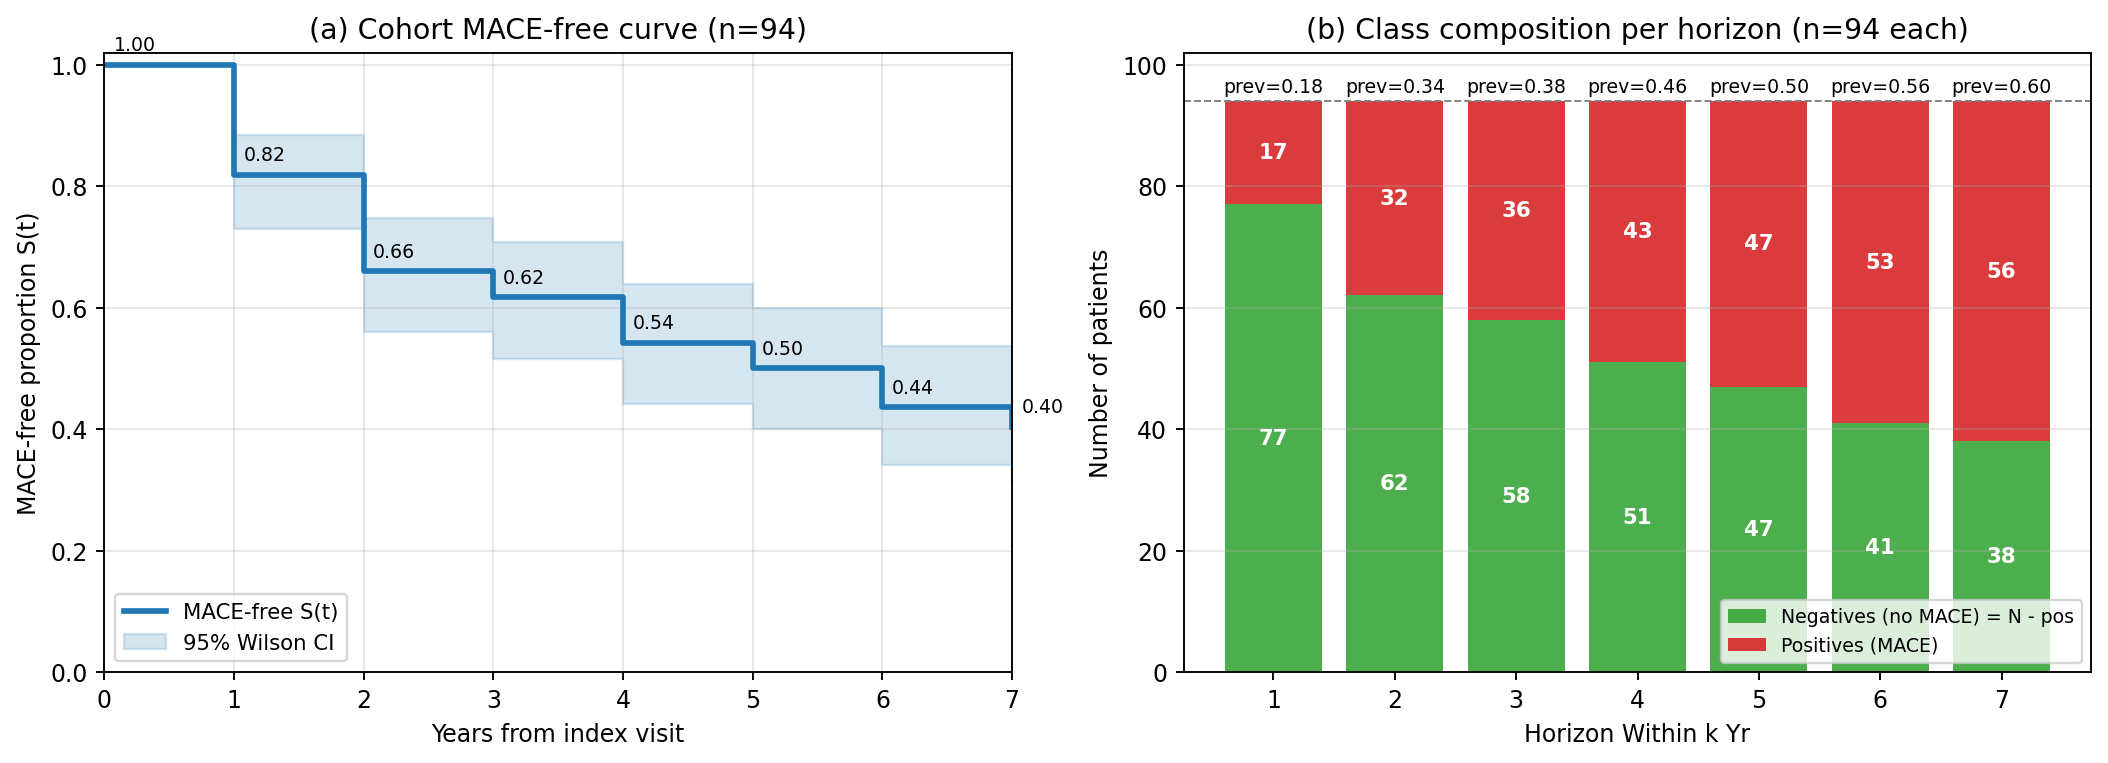
\includegraphics[width=0.98\textwidth]{survival_curve.png}
  \caption{(a) Discrete-time MACE-free curve $S(k)=1-P(\mathrm{MACE}\le k)$
  for the full cohort, step function with Wilson $95\%$ CI band.
  (b) Class composition of the seven binary classification problems:
  every bar sums to $n=94$; the green segment is the negative class
  (event-free at $k$ years) and the red segment is the positive class
  (MACE within $k$ years). E.g.\ Within1Yr has $77$ negatives and $17$
  positives, Within7Yr has $38$ negatives and $56$ positives. This
  motivates anchoring the headline analyses on the latest, most-balanced
  horizon Within7Yr.}
  \label{fig:survival}
\end{figure}

\begin{table}[h]
\centering
\caption{Class composition per horizon. Every horizon uses the same
$n=94$ patients; only the label changes. ``MACE'' counts patients who
experienced an event \emph{within} $k$ years of the index visit;
``no MACE'' counts the complement (event-free at $k$ years).}
\label{tab:prevalence}
\small
\begin{tabular}{lrrrr}
\toprule
Horizon & $n$ (total) & no MACE (negatives) & MACE (positives) & Prevalence \\
\midrule
Within1Yr & 94 & 77 & 17 & 0.18 \\
Within2Yr & 94 & 62 & 32 & 0.34 \\
Within3Yr & 94 & 58 & 36 & 0.38 \\
Within4Yr & 94 & 51 & 43 & 0.46 \\
Within5Yr & 94 & 47 & 47 & 0.50 \\
Within6Yr & 94 & 41 & 53 & 0.56 \\
Within7Yr & 94 & 38 & 56 & 0.60 \\
\bottomrule
\end{tabular}
\end{table}

\subsection{Data preprocessing}
\label{sec:preprocessing}
The \texttt{imputed\_proteomics\_base.csv} file delivered to the
modelling stage already encodes every preprocessing decision that
\emph{precedes} the supervised pipeline:
\begin{itemize}[leftmargin=*]
  \item \textbf{Identifier handling.} \texttt{EuroSCOREPatient ID} is
    treated as a record-only column, never read into the feature matrix.
  \item \textbf{Outcome handling.} The seven \texttt{Within$k$Yr} columns
    are integer $\{0,1\}$ labels; nothing else in the file is interpreted
    as a target.
  \item \textbf{Missingness.} Olink panels and derived analytes are pre-imputed,
    so no imputation step lives inside the supervised pipeline. This avoids
    a common leakage source where imputers are fit on the full sample and
    leak fold-membership through reconstructed values.
  \item \textbf{Standardisation.} A \texttt{StandardScaler} is fit
    \emph{inside every outer training fold} and applied only for
    stability selection (\Cref{sec:stab}); it is not used by the
    Random-Forest classifier, which is scale-invariant.
  \item \textbf{Per-target leakage prophylaxis.} When training the model
    for \texttt{Within$k$Yr}, the other six outcome columns are dropped
    from the feature matrix.
\end{itemize}
The net effect is that every step that learns from the data ---
standardisation and feature selection --- is fold-respecting, while every
step that does not (label encoding, identifier removal, fixed-imputation
read-back) happens once at load time.

\subsection{Per-target framing and label-leakage prophylaxis}
We train seven independent binary classifiers, one per horizon. When
modelling \emph{Within$k$Yr}, the other six outcome columns are removed
from the feature matrix to rule out a particularly insidious form of
label leakage in which short-horizon outcomes implicitly predict
long-horizon outcomes (or vice versa).

\subsection{Nested cross-validation}
Let $\mathcal{D} = \{(\bm{x}_i, y_i)\}_{i=1}^{n}$ with $\bm{x}_i \in
\mathbb{R}^{p}$ and $y_i \in \{0,1\}$. The outer loop is a
$\mathrm{RepeatedStratifiedKFold}(K_\mathrm{out}=5,\,R=3)$ with seed $42$,
yielding $15$ disjoint test partitions $\mathcal{T}_f$ and matching
training partitions $\mathcal{D}_f^{\mathrm{tr}}$. The inner loop is a
$\mathrm{StratifiedKFold}(K_\mathrm{in}=5)$ over $\mathcal{D}_f^{\mathrm{tr}}$
used exclusively for hyperparameter selection. Held-out predictions
$\hat{y}_i^{\mathrm{oof}}$ are produced once per patient per repeat and
pooled across folds for global ROC, PR, calibration and confusion-matrix
analyses.

\subsection{Feature selection: stability selection over an $\ell_1$ grid}
\label{sec:stab}

\paragraph{Approach in plain language.}
With $p=551$ candidates and only $n=94$ patients, any single fit of a
sparse model produces a feature list that depends heavily on which
patients happen to be in the training set, and on the chosen
regularisation strength. The published shortlist therefore has to
satisfy two requirements at once: it must be \emph{reproducible} (the
same features should keep being chosen across resamples), and it must be
\emph{robust} to the choice of regularisation strength (no single
$\lambda$ should be allowed to dictate the answer). \emph{Stability
selection} \cite{} is the standard remedy: fit the sparse model many
times on bootstrap-style subsamples of the data, count how often each
feature receives a non-zero coefficient, and retain only the features
whose selection frequency clears a threshold. We use the
\emph{randomised-lasso} variant, which fits the same logistic regression
across a small grid of regularisation strengths and aggregates by taking
the per-feature \emph{maximum} frequency, so that a feature is kept if
it is reliably picked up at \emph{any} regularisation level rather than
on average across the grid. Concretely:

Inside every outer training fold $f$, we standardise the features
\[
  z_{ij} = \frac{x_{ij} - \mu_j^{(f)}}{\sigma_j^{(f)}}, \qquad
  i \in \mathcal{D}_f^{\mathrm{tr}},\ j=1,\dots,p,
\]
where $\mu_j^{(f)}, \sigma_j^{(f)}$ are estimated on the training fold
\emph{only}, and run the following randomised-lasso variant of stability
selection \cite{}.

For $B=100$ random subsamples of size
$\lfloor 0.75\,|\mathcal{D}_f^{\mathrm{tr}}|\rfloor$ drawn without
replacement, and for each $C \in \{0.01, 0.1, 1.0\}$, we fit an
$\ell_1$-regularised, class-balanced logistic regression
\begin{equation}
  \widehat{\bm{\beta}}_{b,C} \in
  \arg\min_{\bm{\beta}\in\mathbb{R}^{p+1}}
  \;\sum_{i\in S_b}
    w_{y_i}\,
    \log\!\left(1 + \exp\bigl(-y_i\,(\bm{x}_i^\top \bm{\beta} + \beta_0)\bigr)\right)
  \;+\; \frac{1}{C}\,\|\bm{\beta}\|_1,
  \label{eq:l1lr}
\end{equation}
with $w_y$ inverse-frequency class weights, solved with the SAGA solver.
A feature $j$ is recorded as ``selected'' on subsample $b$ at strength
$C$ if $|\widehat{\beta}_{b,C,j}| > 10^{-8}$. The per-strength
\emph{selection frequency} is
\[
  \pi_{j,C}^{(f)} \;=\; \frac{1}{B}\sum_{b=1}^{B}
    \mathbb{1}\bigl[\,|\widehat{\beta}_{b,C,j}|>10^{-8}\,\bigr],
\]
and the feature's stability score aggregates across the regularisation
grid by taking the maximum,
\begin{equation}
  s_j^{(f)} \;=\; \max_{C \in \{0.01, 0.1, 1.0\}} \pi_{j,C}^{(f)}.
  \label{eq:stab}
\end{equation}
Taking the maximum (rather than the average) implements the
\emph{randomised-lasso} variant: a feature is considered stable if at
\emph{any one} regularisation level it is reliably picked up, which is
more sensitive to weak but consistent signals than averaging across the
grid would be. Features with $s_j^{(f)} \ge 0.60$ are retained, with a
floor of $5$ and a ceiling of $50$ features per fold.

\subsection{Classifiers and hyperparameter tuning}
\label{sec:classifiers}

\paragraph{Approach in plain language.}
Reporting a single classifier on a small-$n$, high-$p$ medical dataset
is risky: a number that looks ``good for an RF'' is often the result of
a model-specific advantage rather than evidence about the underlying
signal. We therefore train \emph{four} classifier families on the same
data, the same outer/inner CV splits, the same stability-selection
front-end, the same metric battery, and the same fixed seed; only the
classifier (and its hyperparameter grid) is allowed to vary. Tuning is
done by \emph{nested cross-validation}: the outer
$\mathrm{RepeatedStratifiedKFold}(5,3)$ produces the held-out estimates
we report, and on every outer training fold an inner
$\mathrm{StratifiedKFold}(5)$ is used by \texttt{GridSearchCV}
(\texttt{scoring="roc\_auc"}, \texttt{refit=True}) to pick the best
hyperparameters \emph{without ever touching the outer test fold}. Every
grid is deliberately small: with $n=94$, each additional grid point
widens the inner-CV optimism gap, and the most defensible defence
against tuning-induced overfitting is a parsimonious search space.

\paragraph{Random Forest.}
Class-balanced \texttt{sklearn.ensemble.\-RandomForestClassifier} with a
per-fold seed; trees are scale-invariant, so the standardisation used
for stability selection is dropped before tree training and the forest
acts on the raw selected columns.

\paragraph{XGBoost.}
\texttt{XGBClassifier} with \texttt{objective="binary:logistic"} and
\texttt{tree\_method="hist"}. Class imbalance is handled by setting
\texttt{scale\_pos\_weight}$\,= n_-^{(f)}/n_+^{(f)}$ \emph{per outer
training fold}, where $n_\pm^{(f)}$ are the positive/negative counts in
that fold. Trees are scale-invariant; standardisation is again dropped
before training.

\paragraph{Logistic Regression ($\ell_1$/$\ell_2$).}
Implemented as a \texttt{Pipeline(StandardScaler, LogisticRegression)}
fitted inside every outer fold: scaling is therefore fold-respecting
\emph{a second time} (the L1 selector already standardises). Class
imbalance is handled by \texttt{class\_weight="balanced"}. The grid
covers both $\ell_2$ (\texttt{lbfgs}) and $\ell_1$
(\texttt{liblinear}) penalties --- the latter can apply additional
sparsity \emph{on top of} stability selection. Maximum iteration count
is set to $5000$ to ensure convergence on every fold.

\paragraph{Support Vector Machine (RBF kernel).}
\texttt{Pipeline(StandardScaler, SVC(kernel="rbf", probability=True))}
with \texttt{class\_weight="balanced"}. The Pipeline is mandatory: the
RBF kernel is dominated by the largest-variance features unless inputs
are standardised. Probabilities are Platt-scaled by sklearn so that the
metric battery (Brier, calibration, ROC-AUC) is well defined; the cost
is a small additional inner cross-validation inside the SVM fit.

\paragraph{Hyperparameter grids.}
\Cref{tab:grids} collects the four grids. Every grid is small by
design; combined with the fold-respecting nested CV, the four families
together require no more than a few minutes per outcome on a multi-core
machine.

\begin{table}[h]
\centering
\caption{Hyperparameter grids tuned on the inner $5$-fold stratified CV
(\texttt{scoring="roc\_auc"}). The first three rows describe the same
training data; only the classifier and its grid change.}
\label{tab:grids}
\small
\begin{tabular}{p{3.4cm}p{10.4cm}}
\toprule
Family & Grid \\
\midrule
Random Forest &
\texttt{n\_estimators}$\in\{300\}$,
\texttt{max\_depth}$\in\{\text{None},5\}$,
\texttt{min\_samples\_leaf}$\in\{1,3\}$,
\texttt{max\_features}$\in\{\sqrt{p},\,0.3\}$ \\[2pt]
XGBoost &
\texttt{n\_estimators}$\in\{200,400\}$,
\texttt{max\_depth}$\in\{3,5\}$,
\texttt{learning\_rate}$\in\{0.05,0.1\}$,
\texttt{subsample}$=0.8$,
\texttt{colsample\_bytree}$=0.8$,
\texttt{reg\_lambda}$=1$,
\texttt{min\_child\_weight}$=1$ \\[2pt]
Logistic Regression &
$\{$\texttt{penalty=l2}, \texttt{C}$\in\{0.01,0.1,1,10\}$, \texttt{solver=lbfgs}$\}$
$\;\cup\;$
$\{$\texttt{penalty=l1}, \texttt{C}$\in\{0.1,1,10\}$, \texttt{solver=liblinear}$\}$ \\[2pt]
SVM (RBF) &
\texttt{C}$\in\{0.1,1,10\}$,
\texttt{gamma}$\in\{$\texttt{scale}$,0.01,0.1\}$ \\
\bottomrule
\end{tabular}
\end{table}

For each outer fold $f$ and each family the inner-CV winner
$\widehat{\bm{\theta}}_f$ is refit on the full training fold and used to
score the outer test fold. Each \emph{published} model is obtained by
re-running stability selection on the full dataset and refitting that
family's classifier at the most-frequent $\widehat{\bm{\theta}}_f$
across the $15$ outer folds.

\paragraph{Final-model feature importance.}
Each family's published model exposes a per-feature importance score; the
gradual-training sweep (\Cref{sec:gradual}) re-uses these as the ranking
to walk down. The score is the canonical one for each family:
mean decrease in impurity (\texttt{rf\_importance}) for Random Forest,
gain-based importance (\texttt{xgb\_importance}) for XGBoost,
$|$standardised coefficient$|$ (\texttt{lr\_importance}) for the LR
Pipeline, and permutation importance (\texttt{svm\_importance}: mean drop
in ROC-AUC over $30$ permutations on the full data) for the SVM. The RBF
SVM has no native feature importances, so permutation is the only
defensible global ranking.

\subsection{Gradual-training sweep}
\label{sec:gradual}
The published pipeline retains $30$--$50$ features per horizon. We
introduce a follow-up analysis that asks, separately for each model
family: \emph{at what feature count does held-out generalisation actually
peak?} Let $\mathcal{F}_{m,k} = \texttt{final\_selected\_features.csv}$
for model family $m\in\{\text{RF, XGB, LR, SVM}\}$ and outcome $k$,
sorted in descending order of \emph{that family's} importance score
(\Cref{sec:classifiers}: \texttt{rf\_importance}, \texttt{xgb\_importance},
\texttt{lr\_importance}, \texttt{svm\_importance} respectively). For
every truncation $k = 1, 2, \dots, |\mathcal{F}_{m,k}|$, we re-run the
\emph{same} nested CV (\Cref{sec:classifiers}) restricted to the top-$k$
features and record the full battery of metrics. Pseudocode is given in
\Cref{alg:gradual}.

\begin{algorithm}[h]
\caption{Gradual-training sweep, per family $m$, per outcome.}
\label{alg:gradual}
\begin{algorithmic}[1]
\STATE Load feature ranking $\mathcal{F}_m$ from family $m$'s
       \texttt{final\_selected\_features.csv} sorted by family-$m$ importance.
\FOR{$k = 1$ \TO $|\mathcal{F}_m|$}
  \STATE Restrict feature matrix to the top-$k$ features of $\mathcal{F}_m$.
  \FOR{each outer fold $f \in \{1,\dots,15\}$}
    \STATE Run inner-CV grid search (\Cref{tab:grids}) for family $m$.
    \STATE Refit at the inner-CV winner; predict on the outer test fold.
    \STATE Record per-fold metrics.
  \ENDFOR
  \STATE Pool out-of-fold predictions; record pooled metrics and Youden
         threshold.
\ENDFOR
\STATE Identify, per metric, the $k$ that maximises (or minimises, for
       Brier) the across-fold mean.
\end{algorithmic}
\end{algorithm}

\paragraph{The look-ahead caveat (sharper for some families).}
A methodological point that we emphasise far more than is usual: each
ranking $\mathcal{F}_m$ is computed on the full dataset, which
introduces a small amount of look-ahead because the ranking is informed
by every patient's outcome. We retain this design deliberately ---
clinicians ask about the \emph{published} list, not about an idealised
list re-derived in every fold; and for each $k$ the model is still
trained and evaluated under fold-respecting nested CV, so the
$k$-vs-performance curve is a held-out estimate of the \emph{model}'s
behaviour conditional on a fixed ordering. The interpretation should
therefore be \emph{``how performance varies along that family's
published ranking''}, not fully nested feature selection.

The size of the resulting bias depends on \emph{how tightly the ranking
is coupled to the model's optimisation criterion}. For tree-based
families (RF and XGBoost), the importance score is a coarse summary of
how often a feature is split on, which is well-defined but only mildly
predictive of out-of-fold accuracy. For linear/kernel families (LR and
SVM-RBF), the importance score is essentially a sufficient statistic of
the global model's decision function: $|$standardised coefficient$|$ is
literally the LR's parameter vector, and permutation importance for an
RBF SVM measures, by construction, how much each feature already
contributes to that model's held-out accuracy. Selecting the
top-$k$ features by such a score and then refitting the same family is
much closer to ``recover the global model'' than for trees. We make
this concrete in \Cref{sec:cross_model_compare}: the gradual peaks
for RF and XGB sit a few points of AUC \emph{above} the unbiased
main-pipeline pooled values, while the gradual peaks for LR and SVM
approach $1.0$. We therefore report the \emph{main-pipeline} numbers as
the headline of the paper, and treat the gradual sweeps as a
sensitivity-on-rank analysis that is most informative for the
tree-based families.

\subsection{Metrics}
At threshold $\tau$ we compute, from the pooled OOF predictions and per
fold,
\begin{equation*}
  \text{ROC-AUC},\
  \text{AP},\
  \text{Acc},\
  \text{BalAcc},\
  F_1,\
  \text{Sens},\
  \text{Spec},\
  \text{Brier},
\end{equation*}
all with their standard sklearn definitions. Two thresholds are reported:
$\tau=0.50$ and the Youden-optimal
$\tau^\star = \arg\max_{\tau} \bigl[\text{TPR}(\tau) - \text{FPR}(\tau)\bigr]$.

\subsection{Reproducibility}
A single \texttt{RANDOM\_STATE = 42} is propagated to every stochastic
component (subsamples, fold splits, and per-fold model seeds via
\texttt{RANDOM\_STATE + fold\_index}). All artefacts --- per-patient OOF
predictions, fold-level metrics, fitted models, plots --- are written to
disk; nothing important lives only in memory.

% =============================================================================
\section{Results}
\label{sec:results}

\subsection{Headline performance: Random Forest (anchor model)}
\Cref{tab:headline} summarises per-horizon out-of-fold performance for
the Random-Forest model at $\tau=0.50$. Pooled ROC-AUC ranges from
$0.64$ at one year to $0.72$ at seven years, broadly matching the
difficulty of the longest horizon having the most balanced classes
(\Cref{tab:prevalence}). Per-fold means with their standard deviations
are reported in the columns labelled ``mean$\pm$sd''.

\begin{table}[h]
\centering
\caption{Main-pipeline pooled performance (15-fold nested CV) per horizon
for the Random-Forest model. \textit{$|\mathcal{F}|$} is the number of
features retained by stability selection on the full data.}
\label{tab:headline}
\small
\begin{tabular}{lrrrrrr}
\toprule
Horizon & $|\mathcal{F}|$ & Pooled AUC & Pooled AP & BalAcc (mean$\pm$sd) & Sens & Spec \\
\midrule
Within1Yr & 33 & 0.636 & 0.286 & 0.495 $\pm$ 0.045 & 0.027 & 0.974 \\
Within2Yr & 50 & 0.637 & 0.469 & 0.587 $\pm$ 0.109 & 0.387 & 0.845 \\
Within3Yr & 48 & 0.695 & 0.586 & 0.614 $\pm$ 0.111 & 0.452 & 0.848 \\
Within4Yr & 38 & 0.660 & 0.689 & 0.590 $\pm$ 0.062 & 0.528 & 0.685 \\
Within5Yr & 46 & 0.693 & 0.722 & 0.645 $\pm$ 0.082 & 0.634 & 0.666 \\
Within6Yr & 50 & 0.714 & 0.782 & 0.632 $\pm$ 0.122 & 0.702 & 0.517 \\
Within7Yr & 49 & 0.719 & 0.792 & 0.644 $\pm$ 0.093 & 0.747 & 0.479 \\
\bottomrule
\end{tabular}
\end{table}

Per-fold AUCs are noticeably variable
($\pm 0.07$--$0.10$), consistent with the small $n$, but the pooled
curves and their AUCs --- which we visualise per horizon below
(\Cref{fig:roc_grid} for the six shorter horizons,
\Cref{fig:within7yr_main} for Within7Yr) --- provide a stable estimate.

\subsection{Cross-model comparison (main pipeline)}
\label{sec:cross_model_compare}

We now broaden the picture to all four families. Recall that the data,
the outer/inner CV splits, the stability-selection front-end, the inner-CV
scoring metric (\texttt{roc\_auc}), the random seed, and the per-outcome
output schema are held \emph{exactly} fixed across the four families;
the only thing that changes is the classifier and its hyperparameter
grid (\Cref{tab:grids}). Differences in the headline numbers below are
therefore attributable to the model rather than to confounded
preprocessing or split choices.

\Cref{tab:cross_model_main} reports pooled out-of-fold AUC, pooled
average precision, per-fold mean balanced accuracy, and pooled Brier
score for representative horizons, and \Cref{fig:cross_model_main}
visualises the trends across all seven horizons. Three observations
stand out:
\begin{enumerate}[leftmargin=*]
  \item \emph{The four families are broadly comparable.} On every
    horizon the pooled AUC range across the four families is roughly
    $0.06$, well within the per-fold standard deviation. Headline
    performance is data-limited, not model-limited.
  \item \emph{Tree-based models lead at the longer, more balanced
    horizons.} Random Forest is the strongest single model at
    Within7Yr ($0.72$ pooled AUC), with XGBoost closely matched.
  \item \emph{Linear and kernel models are competitive at the shortest,
    most imbalanced horizon.} On Within1Yr (prevalence $0.18$),
    SVM-RBF and Logistic Regression match or slightly exceed the
    Random-Forest pooled AUC, suggesting that regularised decision
    boundaries handle the very-low-positive-count regime at least as
    well as bagging.
\end{enumerate}
Pooled Brier scores are uniformly best for the tree-based families
(\Cref{fig:cross_model_brier}); the linear and kernel models, despite
similar AUC, are noticeably less well calibrated at $\tau=0.50$, which
points at a future calibration-recalibration step (Platt or isotonic).

\begin{table}[h]
\centering
\caption{Cross-model main-pipeline pooled out-of-fold performance for
four representative horizons. ``BalAcc'' is the per-fold mean of
balanced accuracy across the $15$ outer folds. The four families share
every preprocessing and validation choice; only the classifier varies
(\Cref{tab:grids}).}
\label{tab:cross_model_main}
\small
\begin{tabular}{llrrrrr}
\toprule
Horizon & Family & $|\mathcal{F}|$ & Pooled AUC & Pooled AP & BalAcc (mean) & Brier \\
\midrule
Within1Yr & Random Forest       & 33 & 0.636 & 0.286 & 0.495 & 0.149 \\
          & XGBoost             & 33 & 0.596 & 0.253 & 0.552 & 0.181 \\
          & Logistic Regression & 33 & 0.634 & 0.299 & 0.599 & 0.185 \\
          & SVM-RBF             & 33 & 0.654 & 0.292 & 0.552 & 0.171 \\
\midrule
Within3Yr & Random Forest       & 48 & 0.695 & 0.586 & 0.614 & 0.209 \\
          & XGBoost             & 48 & 0.685 & 0.591 & 0.621 & 0.244 \\
          & Logistic Regression & 48 & 0.710 & 0.622 & 0.661 & 0.245 \\
          & SVM-RBF             & 48 & 0.686 & 0.627 & 0.634 & 0.260 \\
\midrule
Within5Yr & Random Forest       & 46 & 0.693 & 0.722 & 0.645 & 0.221 \\
          & XGBoost             & 46 & 0.705 & 0.727 & 0.621 & 0.254 \\
          & Logistic Regression & 46 & 0.636 & 0.653 & 0.565 & 0.310 \\
          & SVM-RBF             & 46 & 0.631 & 0.647 & 0.573 & 0.314 \\
\midrule
Within7Yr & Random Forest       & 49 & 0.719 & 0.792 & 0.644 & 0.205 \\
          & XGBoost             & 49 & 0.696 & 0.749 & 0.645 & 0.242 \\
          & Logistic Regression & 49 & 0.679 & 0.751 & 0.634 & 0.254 \\
          & SVM-RBF             & 49 & 0.657 & 0.758 & 0.583 & 0.273 \\
\bottomrule
\end{tabular}
\end{table}

\begin{figure}[h]
  \centering
  \begin{subfigure}[t]{0.49\textwidth}
    \centering
    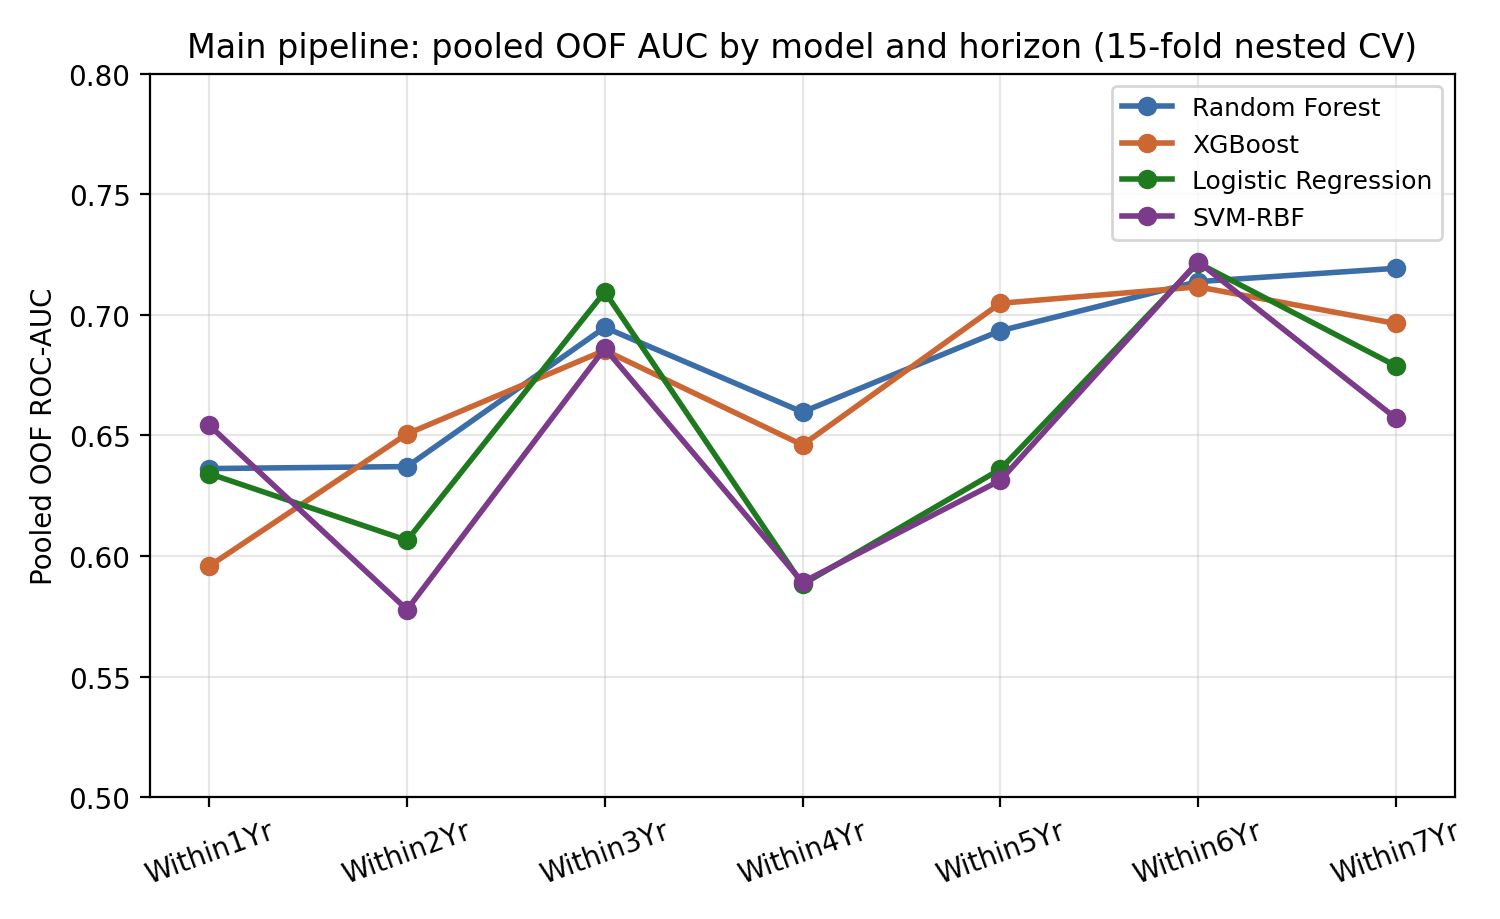
\includegraphics[width=\linewidth]{compare_models_pooled_auc.png}
    \caption{Pooled out-of-fold ROC-AUC.}
    \label{fig:cross_model_pooled_auc}
  \end{subfigure}
  \hfill
  \begin{subfigure}[t]{0.49\textwidth}
    \centering
    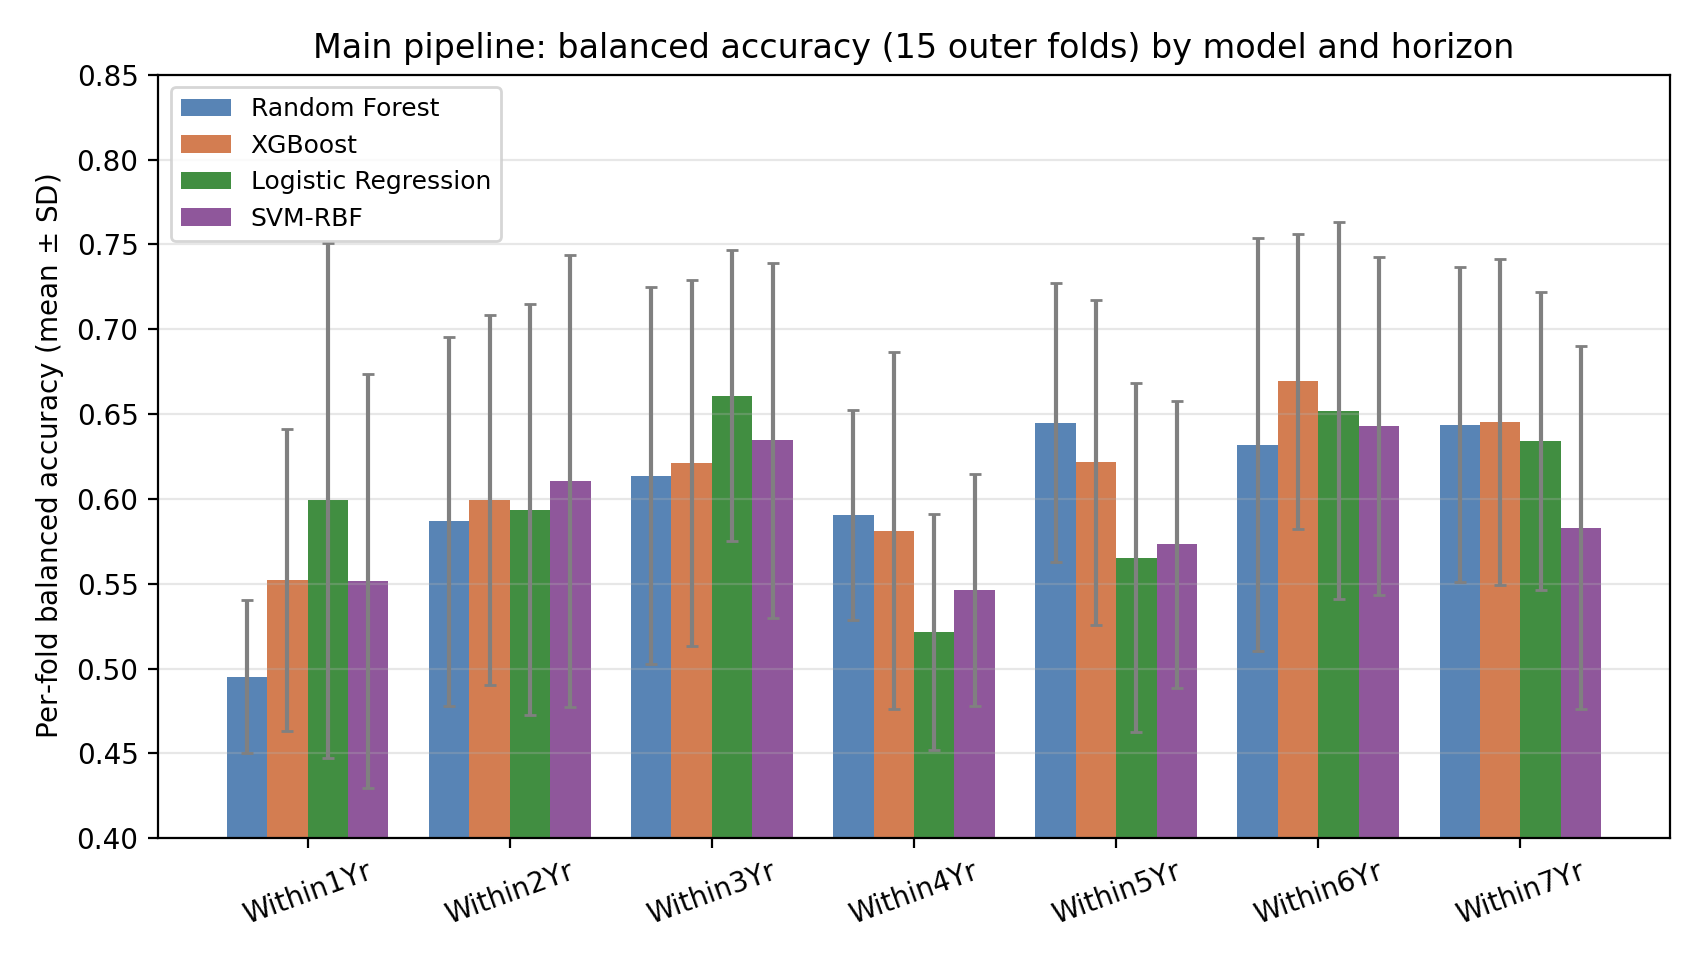
\includegraphics[width=\linewidth]{compare_models_balacc.png}
    \caption{Per-fold balanced accuracy (mean $\pm$ SD across $15$
    outer folds).}
    \label{fig:cross_model_balacc}
  \end{subfigure}
  \caption{Cross-model comparison under the main pipeline. (a) The four
  families track one another closely; the spread at any horizon is
  roughly $0.06$ AUC, smaller than the per-fold SD. (b) Balanced
  accuracy bars show the same broad agreement, with the SVM noticeably
  lower at the most balanced (Within7Yr) horizon.}
  \label{fig:cross_model_main}
\end{figure}

\begin{figure}[h]
  \centering
  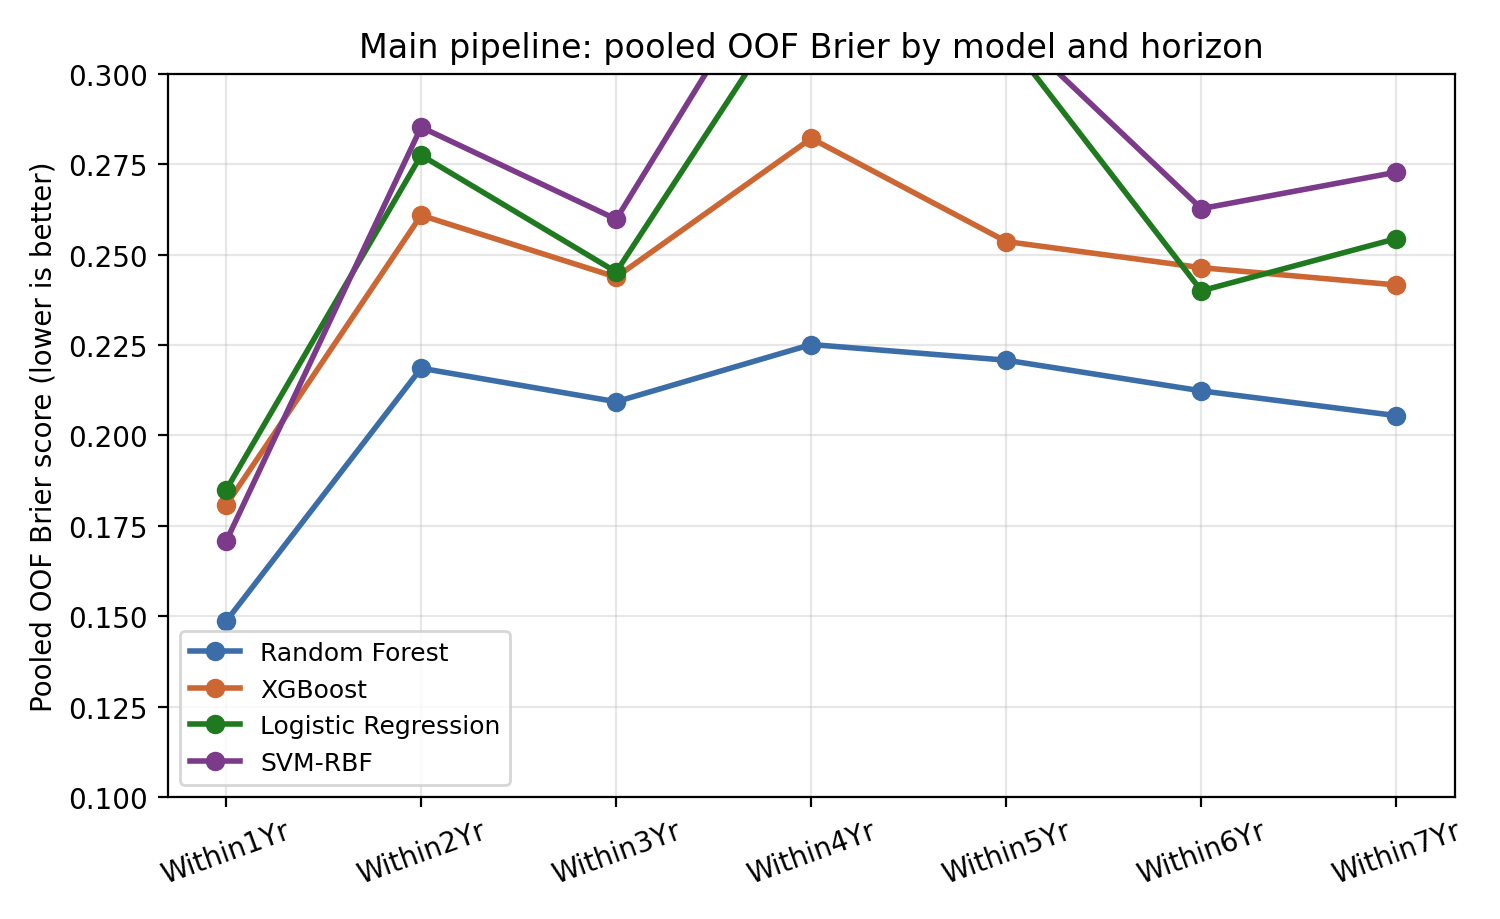
\includegraphics[width=0.74\textwidth]{compare_models_brier.png}
  \caption{Pooled out-of-fold Brier score by family and horizon (lower
  is better). Tree-based families (RF, XGB) are uniformly better
  calibrated at $\tau=0.50$ than the linear / kernel families (LR,
  SVM-RBF). All four families benefit from a future
  calibration-recalibration step.}
  \label{fig:cross_model_brier}
\end{figure}

\subsection{Cross-model gradual sweep and the look-ahead gap}
\label{sec:cross_model_gradual}

\Cref{fig:cross_model_peak_auc} plots the gradual peak per-fold mean AUC
for each family at each horizon. Read on its own, this figure looks
spectacular --- LR and SVM-RBF reach peaks above $0.95$ on every
horizon. Read against the unbiased main-pipeline pooled AUC of
\Cref{fig:cross_model_pooled_auc} --- which is the same data, the same
folds, the same seed --- those numbers tell a different story.

\begin{figure}[h]
  \centering
  \begin{subfigure}[t]{0.49\textwidth}
    \centering
    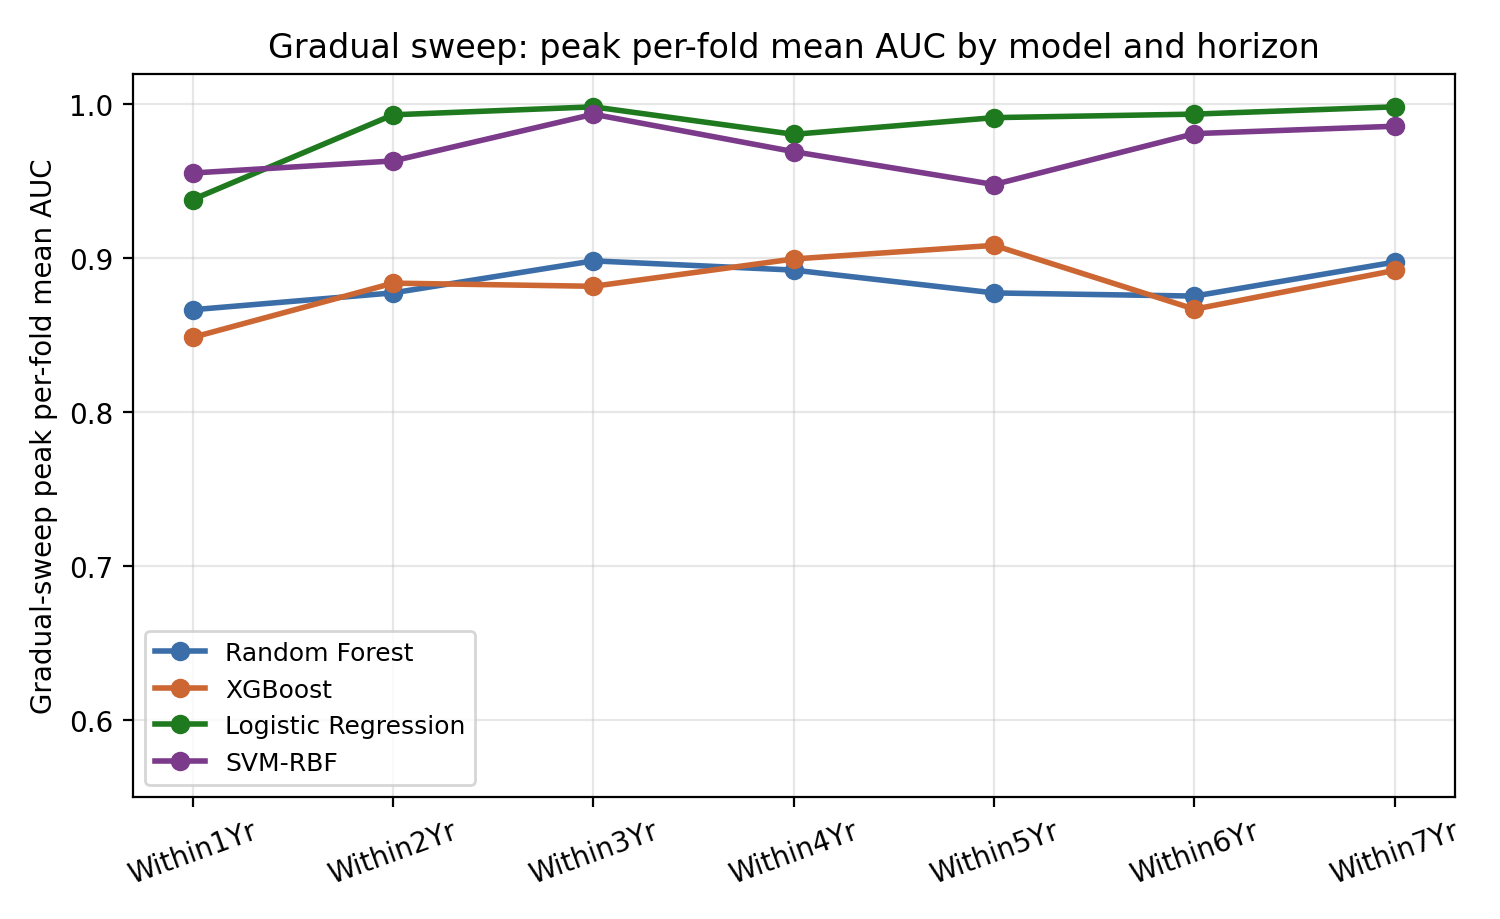
\includegraphics[width=\linewidth]{compare_models_peak_auc.png}
    \caption{Gradual sweep peak AUC.}
    \label{fig:cross_model_peak_auc}
  \end{subfigure}
  \hfill
  \begin{subfigure}[t]{0.49\textwidth}
    \centering
    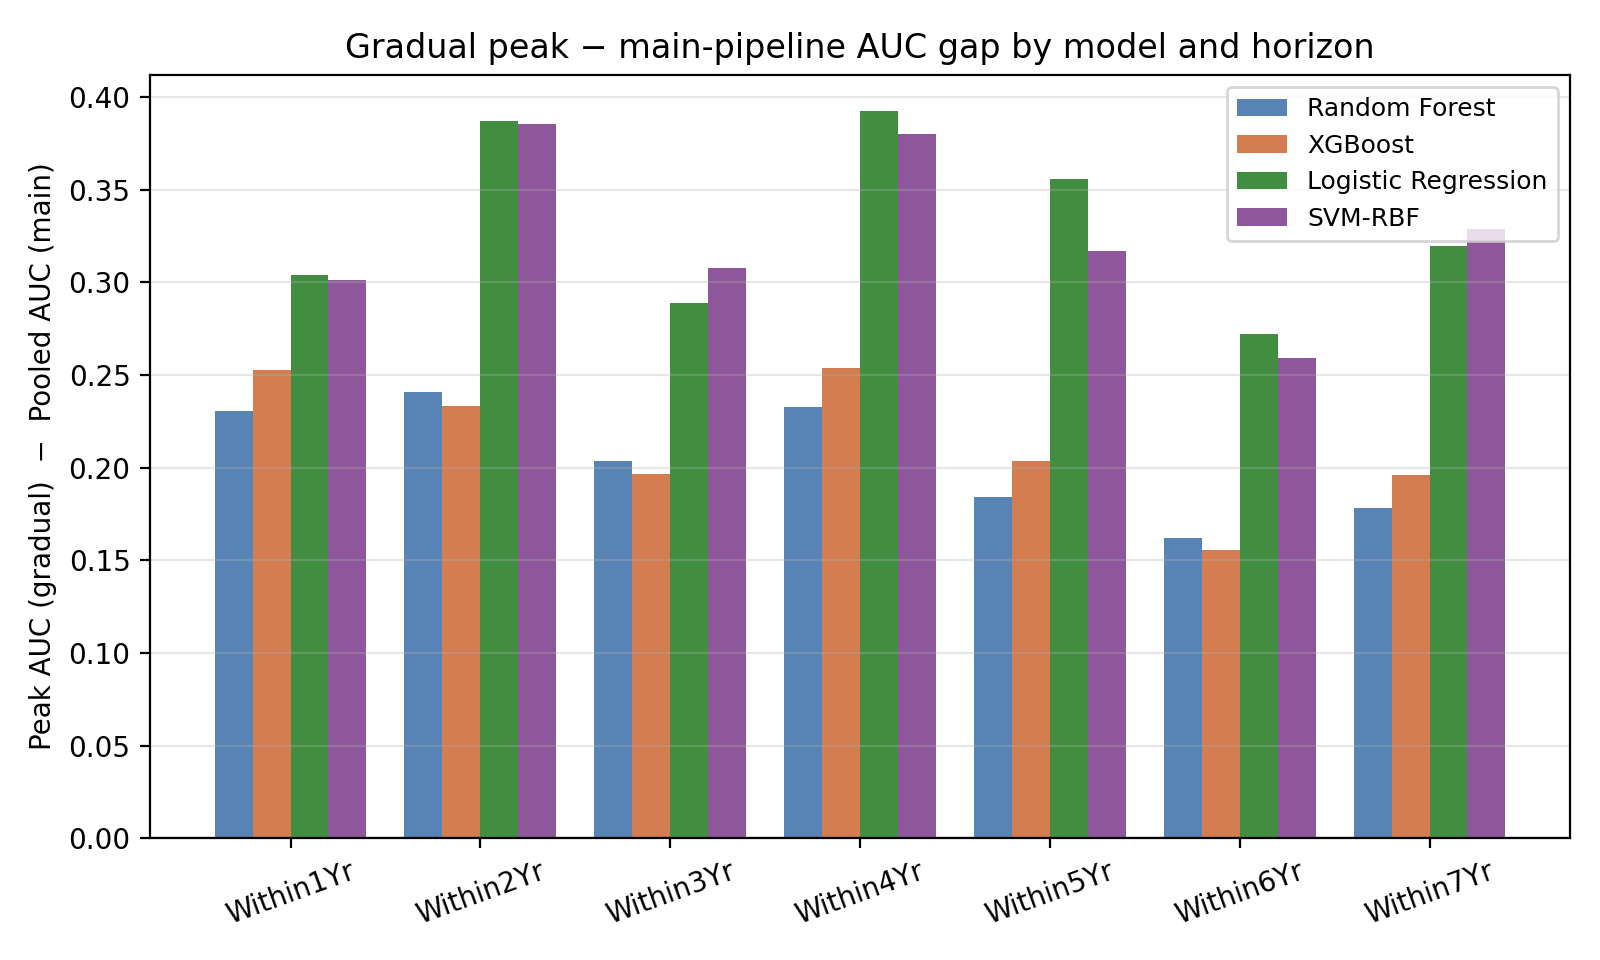
\includegraphics[width=\linewidth]{compare_models_peak_minus_pooled.png}
    \caption{Peak (gradual) $-$ pooled (main) AUC.}
    \label{fig:cross_model_gap}
  \end{subfigure}
  \caption{Look-ahead size by family. (a) Peak per-fold mean AUC reached
  by each family's gradual sweep across horizons. (b) The same numbers
  expressed as a gap relative to the unbiased main-pipeline pooled AUC.
  The tree-based families (RF, XGB) sit roughly $0.15$--$0.25$ above
  their main-pipeline pooled AUC; the linear / kernel families (LR,
  SVM) sit roughly $0.30$--$0.40$ above. The latter is the size of the
  rank-induced look-ahead, not a real predictive improvement.}
  \label{fig:cross_model_gradual}
\end{figure}

\Cref{tab:cross_model_gradual} reports the gradual peaks alongside their
matching main-pipeline values. The mechanism, restated from
\Cref{sec:gradual}: each family's published feature ranking is computed
on the full dataset, including the patients in every test fold; selecting
the top-$k$ features by that ranking and re-evaluating the \emph{same
family} under nested CV recovers a noticeably more optimistic curve than
running the full pipeline cleanly. The bias is small and benign for tree
importances ($+0.15$--$0.25$ AUC), and \emph{very} large for linear and
kernel importances ($+0.30$--$0.40$ AUC), because in those cases the
ranking score is itself a sufficient statistic of the global model's
decision function (\Cref{sec:gradual}).

\begin{table}[h]
\centering
\caption{Gradual peak AUC vs.\ main-pipeline pooled AUC, per family per
horizon. ``$\Delta$'' is the gap induced by the rank-on-full-data
look-ahead: small for trees, large for linear / kernel models.}
\label{tab:cross_model_gradual}
\small
\begin{tabular}{ll rrr rrr}
\toprule
& & \multicolumn{3}{c}{Within3Yr} & \multicolumn{3}{c}{Within7Yr} \\
\cmidrule(lr){3-5}\cmidrule(lr){6-8}
Family & $|\mathcal{F}|$
       & Pool. AUC & Peak AUC ($k^\star$) & $\Delta$
       & Pool. AUC & Peak AUC ($k^\star$) & $\Delta$ \\
\midrule
Random Forest       & 48/49 & 0.695 & 0.898 ($k\!=\!34$) & $+0.20$ & 0.719 & 0.898 ($k\!=\!26$) & $+0.18$ \\
XGBoost             & 48/49 & 0.685 & 0.882 ($k\!=\!31$) & $+0.20$ & 0.696 & 0.892 ($k\!=\!28$) & $+0.20$ \\
Logistic Regression & 48/49 & 0.710 & 0.998 ($k\!=\!31$) & $+0.29$ & 0.679 & 0.998 ($k\!=\!40$) & $+0.32$ \\
SVM-RBF             & 48/49 & 0.686 & 0.994 ($k\!=\!38$) & $+0.31$ & 0.657 & 0.986 ($k\!=\!48$) & $+0.33$ \\
\bottomrule
\end{tabular}
\end{table}

\paragraph{Practical consequence.}
We therefore treat the gradual sweep as a \emph{sensitivity analysis on
the published ranking}, not as a held-out estimate of model performance.
Two more concrete consequences:
\begin{itemize}[leftmargin=*]
  \item For the tree-based families, the ``parsimony'' interpretation of
    the gradual sweep is intact: the curve plateaus or peaks well before
    $|\mathcal{F}|$, which is qualitative evidence that the long tail of
    the published list is dispensable. Quantitatively, the peak height
    is overstated by $0.15$--$0.25$ AUC, so the headline parsimony claim
    is real but the magnitudes should not be quoted as held-out
    accuracy.
  \item For the linear / kernel families, the gradual sweep should be
    read \emph{only} as a description of the published ranking's shape;
    its peak value is essentially a re-derivation of the global model
    fitted on the full data and carries no held-out information.
\end{itemize}
This is also why we anchor the within7Yr walkthrough
(\Cref{sec:within7yr}) on the Random Forest: it is the family for which
the gradual sweep is most informative as a parsimony argument.

\subsection{Per-horizon comparison (Within1Yr--Within6Yr in brief)}
\label{sec:per_horizon}

Before zooming in on Within7Yr, we briefly walk through the held-out
behaviour of each shorter-horizon classifier. \Cref{fig:compare_auc}
shows pooled and per-fold-mean ROC-AUC across the seven horizons under
the main pipeline; \Cref{fig:compare_peak} shows the corresponding peak
AUC reached by the gradual sweep, together with the optimal feature
count $k^\star$.

\begin{figure}[h]
  \centering
  \begin{subfigure}[t]{0.49\textwidth}
    \centering
    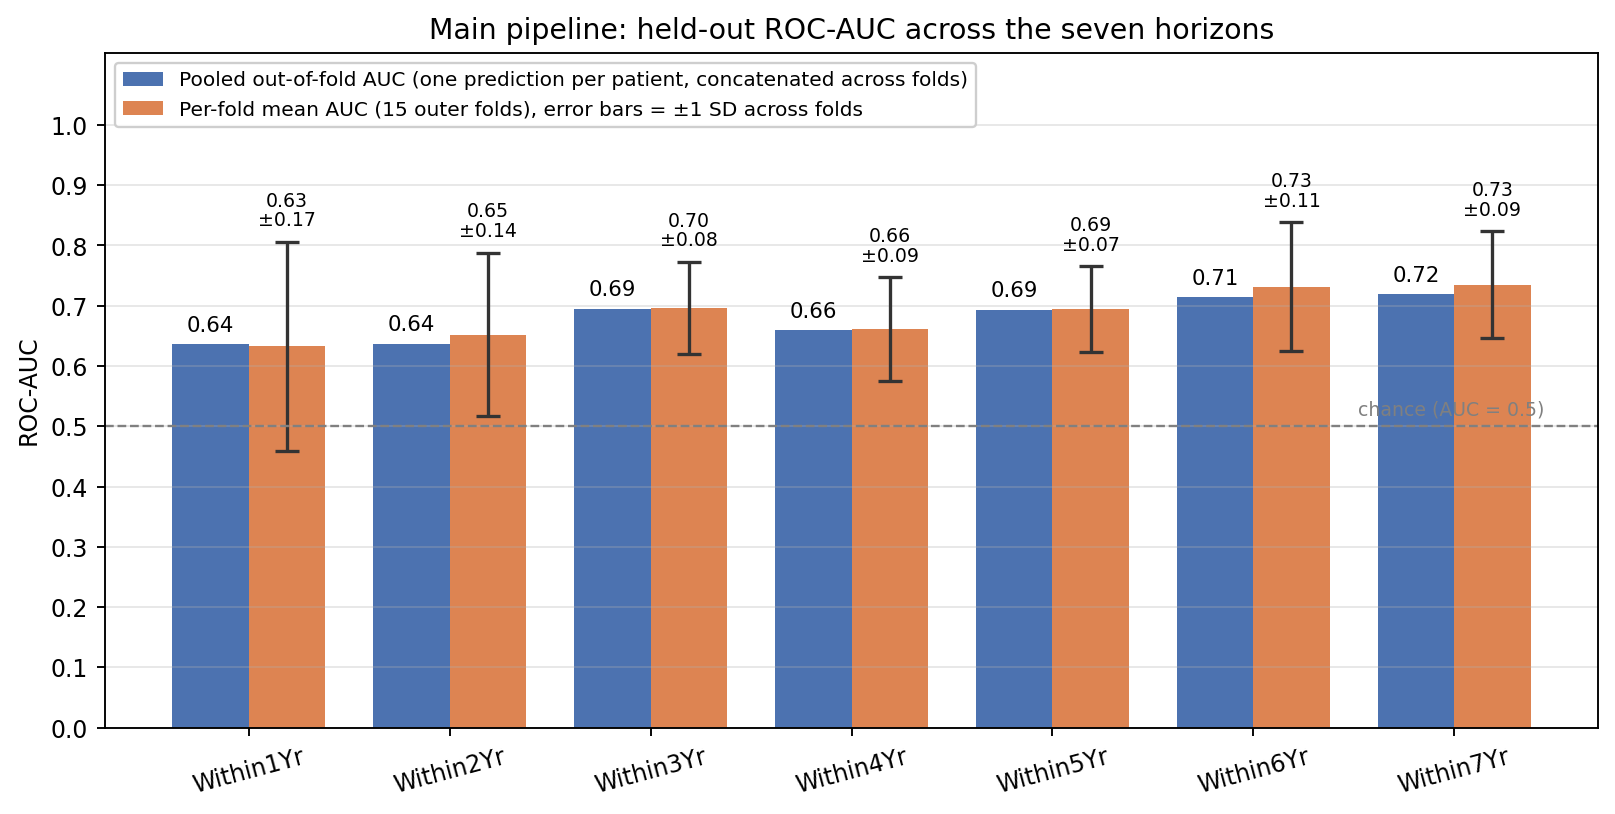
\includegraphics[width=\linewidth]{compare_auc_horizons.png}
    \caption{Main pipeline.}
    \label{fig:compare_auc}
  \end{subfigure}
  \hfill
  \begin{subfigure}[t]{0.49\textwidth}
    \centering
    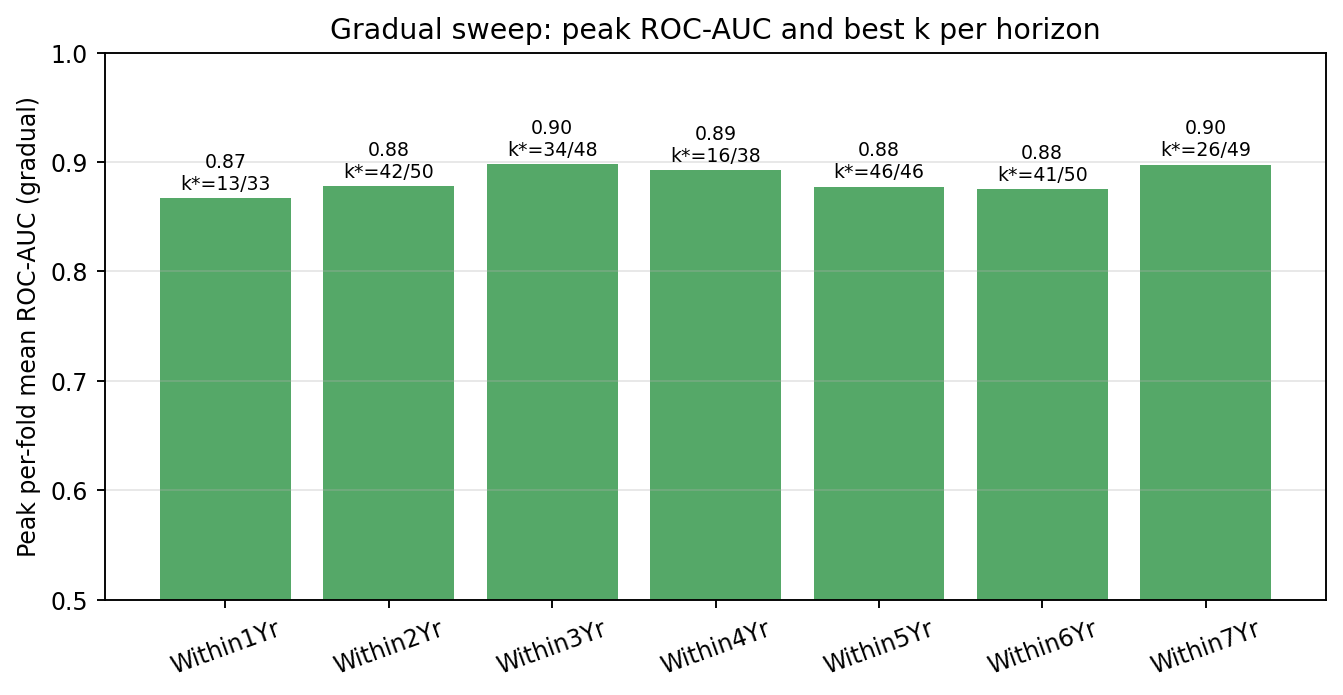
\includegraphics[width=\linewidth]{compare_peakauc_horizons.png}
    \caption{Gradual sweep peaks.}
    \label{fig:compare_peak}
  \end{subfigure}
  \caption{Cross-classifier comparison. (a) Held-out ROC-AUC of the
  $|\mathcal{F}|$-feature published model per horizon: pooled
  out-of-fold curve and per-fold mean$\pm$SD. (b) Peak per-fold mean
  ROC-AUC reached by the gradual sweep at the best feature count
  $k^\star$ ($k^\star/|\mathcal{F}|$ printed above each bar).}
\end{figure}

\Cref{fig:roc_grid} contrasts the per-fold and pooled ROC curves of all
six shorter horizons in a single grid; the corresponding gradual
all-metric panels are shown in \Cref{fig:gradual_grid}. Per-classifier
take-aways:
\begin{itemize}[leftmargin=*]
  \item \textbf{Within1Yr} ($\mathit{prev}\!=\!0.18$, $|\mathcal{F}|=33$).
    Pooled AUC $0.636$, per-fold mean $0.49\pm 0.05$ balanced accuracy.
    The model essentially defaults to the majority class at $\tau=0.5$
    (sensitivity $0.03$, specificity $0.97$), and only the
    Youden-optimal threshold recovers a usable operating point. The
    gradual peak is encouraging (AUC $0.867$ at $k=13$) but is computed
    on the bumpiest curve in the panel and should be interpreted with
    the largest grain of salt.
  \item \textbf{Within2Yr} ($\mathit{prev}\!=\!0.34$, $|\mathcal{F}|=50$).
    Pooled AUC $0.637$, balanced accuracy $0.59$. Classes are now closer
    to balanced; the gradual sweep peaks at AUC $0.878$ for $k=42$.
  \item \textbf{Within3Yr} ($\mathit{prev}\!=\!0.38$, $|\mathcal{F}|=48$).
    Pooled AUC $0.695$, the first clearly above-chance pooled estimate.
    Discussed in detail in \Cref{sec:gradual_within3yr_subsec}.
  \item \textbf{Within4Yr} ($\mathit{prev}\!=\!0.46$, $|\mathcal{F}|=38$).
    Pooled AUC $0.660$, but balanced accuracy is the most stable so far
    ($0.59\pm 0.06$); gradual peak balanced accuracy $0.81$ at $k=17$
    is the highest of any horizon.
  \item \textbf{Within5Yr} ($\mathit{prev}\!=\!0.50$, $|\mathcal{F}|=46$).
    Pooled AUC $0.693$, balanced accuracy $0.64\pm 0.08$. Best $k$ for
    balanced accuracy is $8$ --- the smallest of any horizon, suggesting
    a very compact subset already captures most of the signal at this
    horizon.
  \item \textbf{Within6Yr} ($\mathit{prev}\!=\!0.56$, $|\mathcal{F}|=50$).
    Pooled AUC $0.714$, peak $F_1$ at $k=13$ of $0.82$. The closest
    competitor to Within7Yr.
\end{itemize}

\begin{figure}[h]
  \centering
  \begin{subfigure}[t]{0.32\textwidth}
    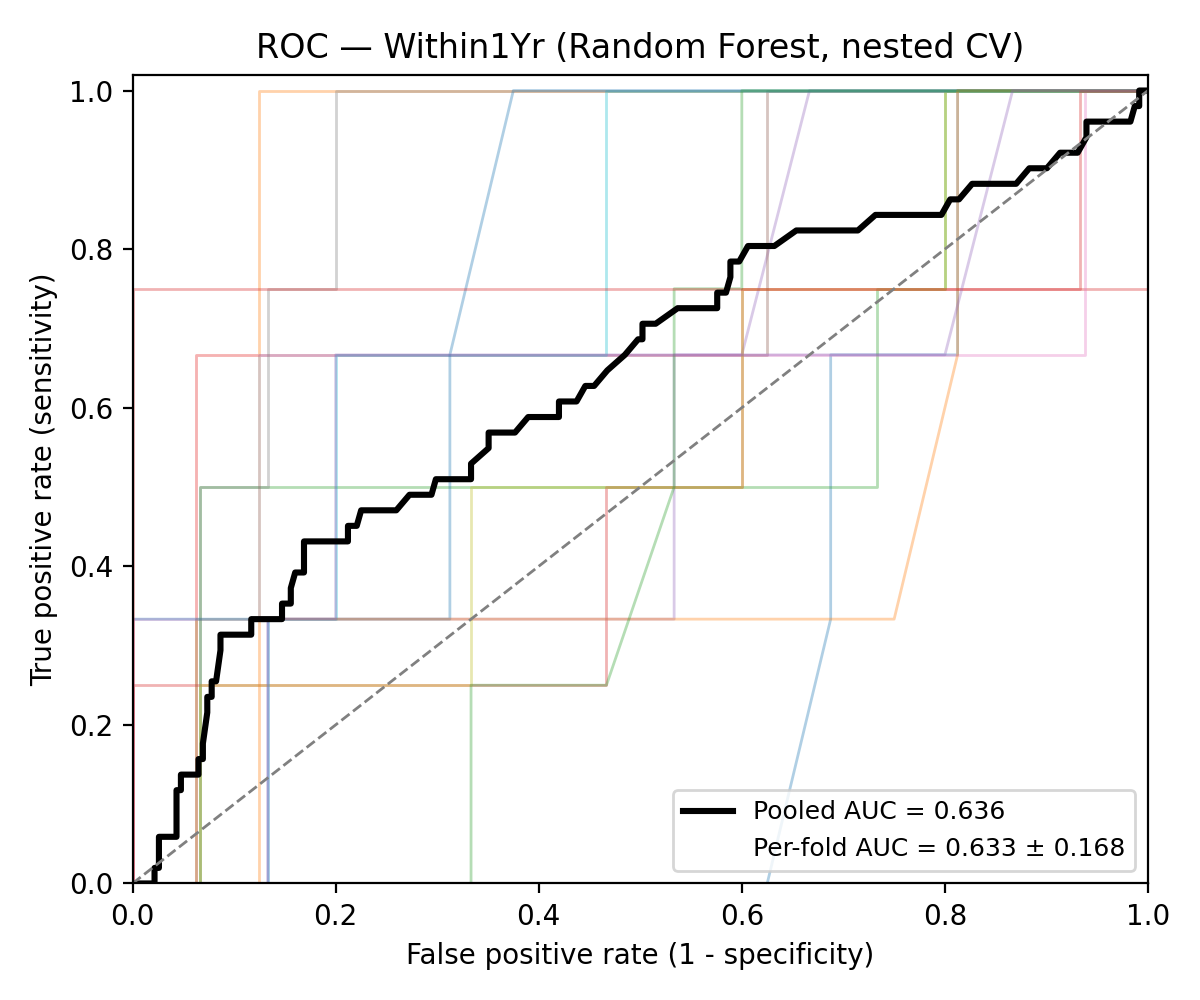
\includegraphics[width=\linewidth]{main_roc_within1yr.png}
    \caption{Within1Yr.}
  \end{subfigure}
  \begin{subfigure}[t]{0.32\textwidth}
    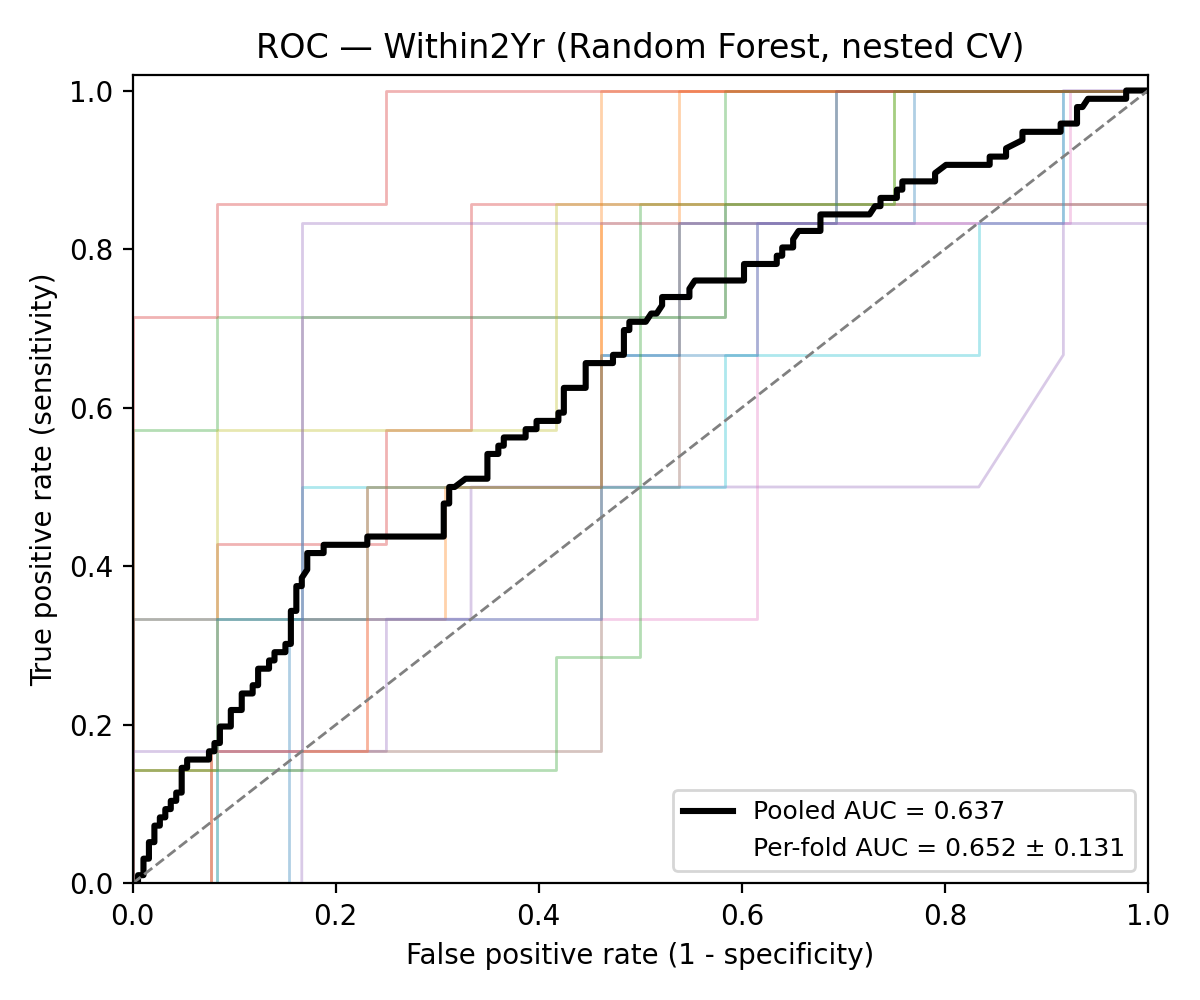
\includegraphics[width=\linewidth]{main_roc_within2yr.png}
    \caption{Within2Yr.}
  \end{subfigure}
  \begin{subfigure}[t]{0.32\textwidth}
    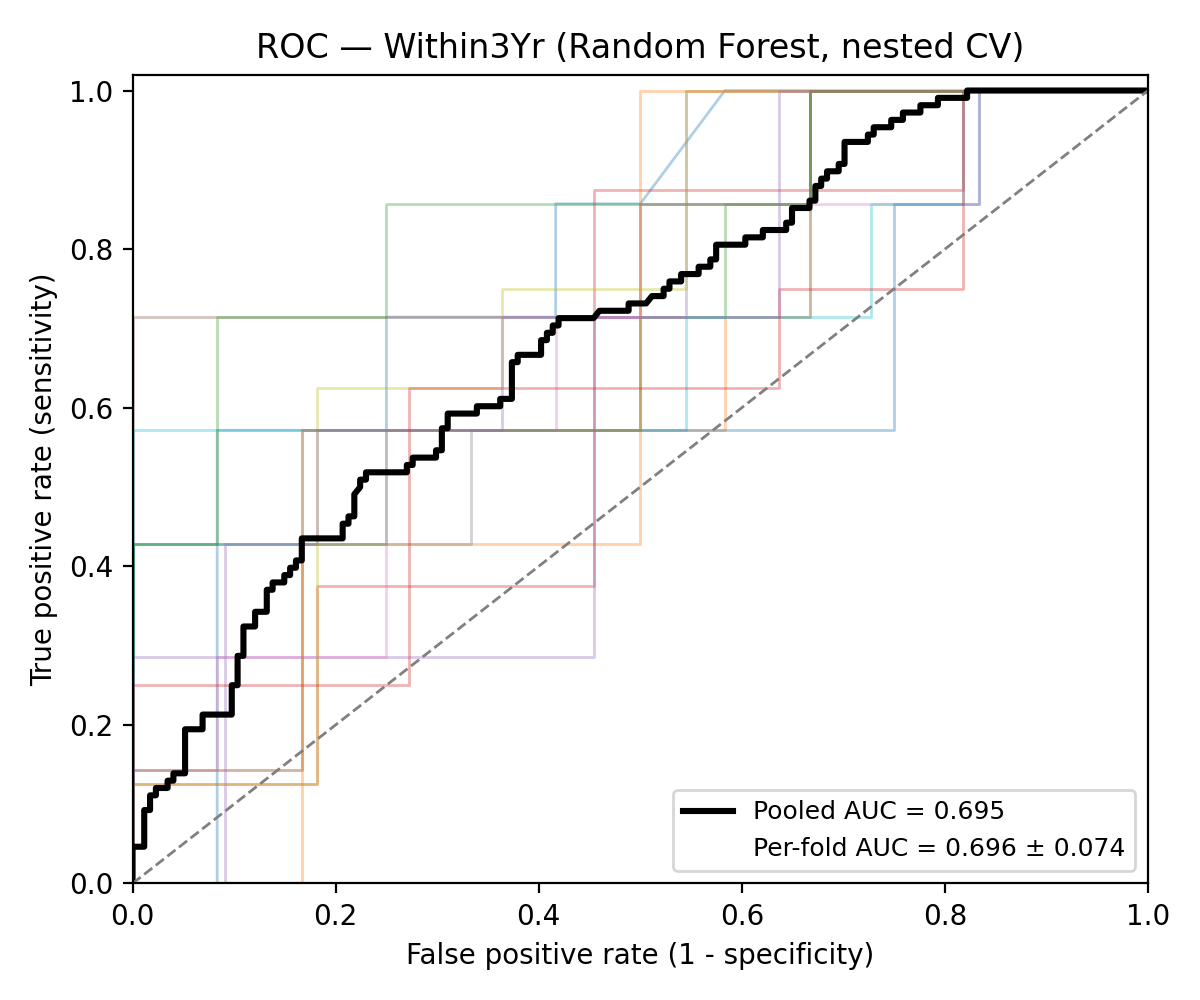
\includegraphics[width=\linewidth]{main_roc_within3yr.png}
    \caption{Within3Yr.}
  \end{subfigure}\\
  \begin{subfigure}[t]{0.32\textwidth}
    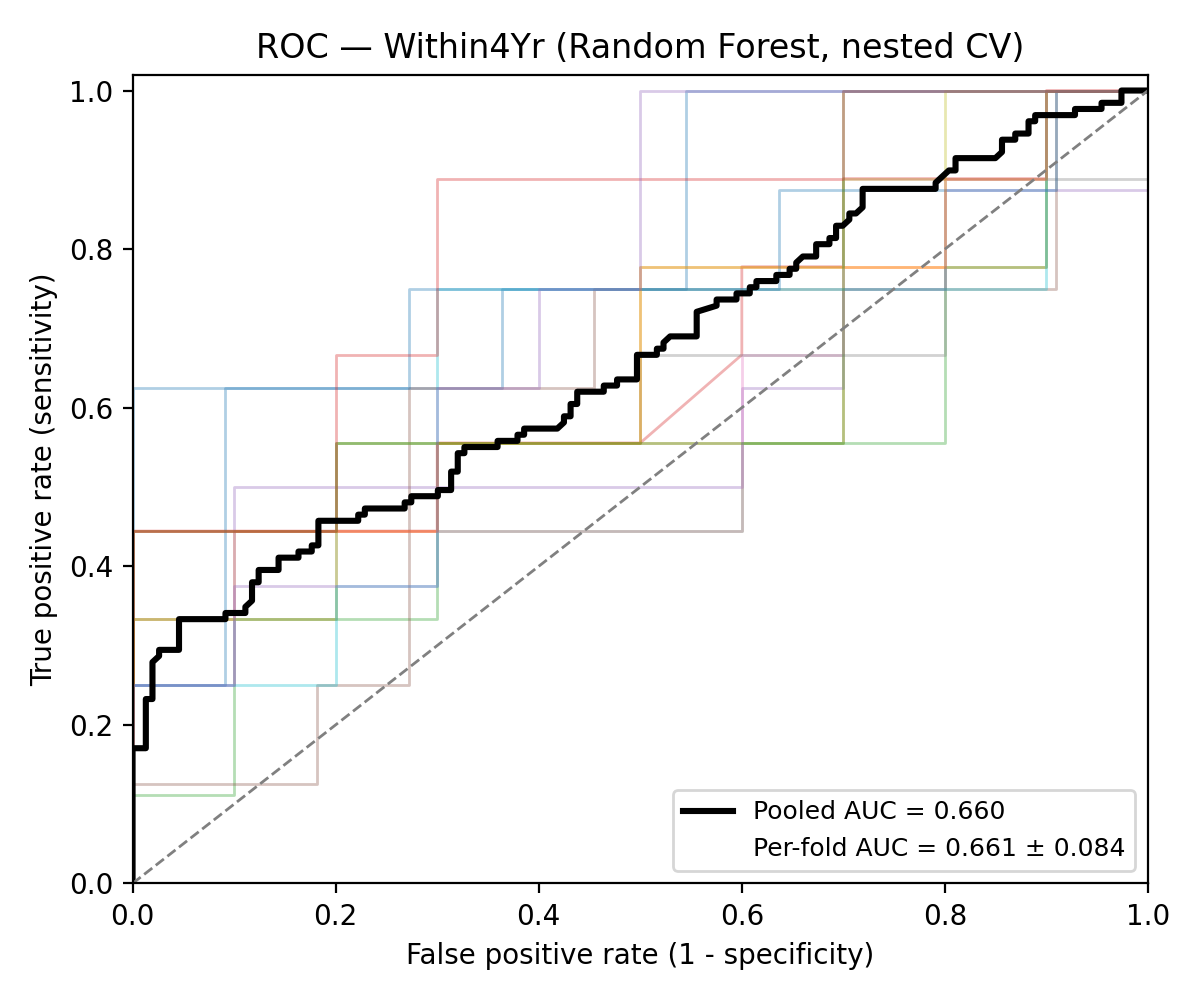
\includegraphics[width=\linewidth]{main_roc_within4yr.png}
    \caption{Within4Yr.}
  \end{subfigure}
  \begin{subfigure}[t]{0.32\textwidth}
    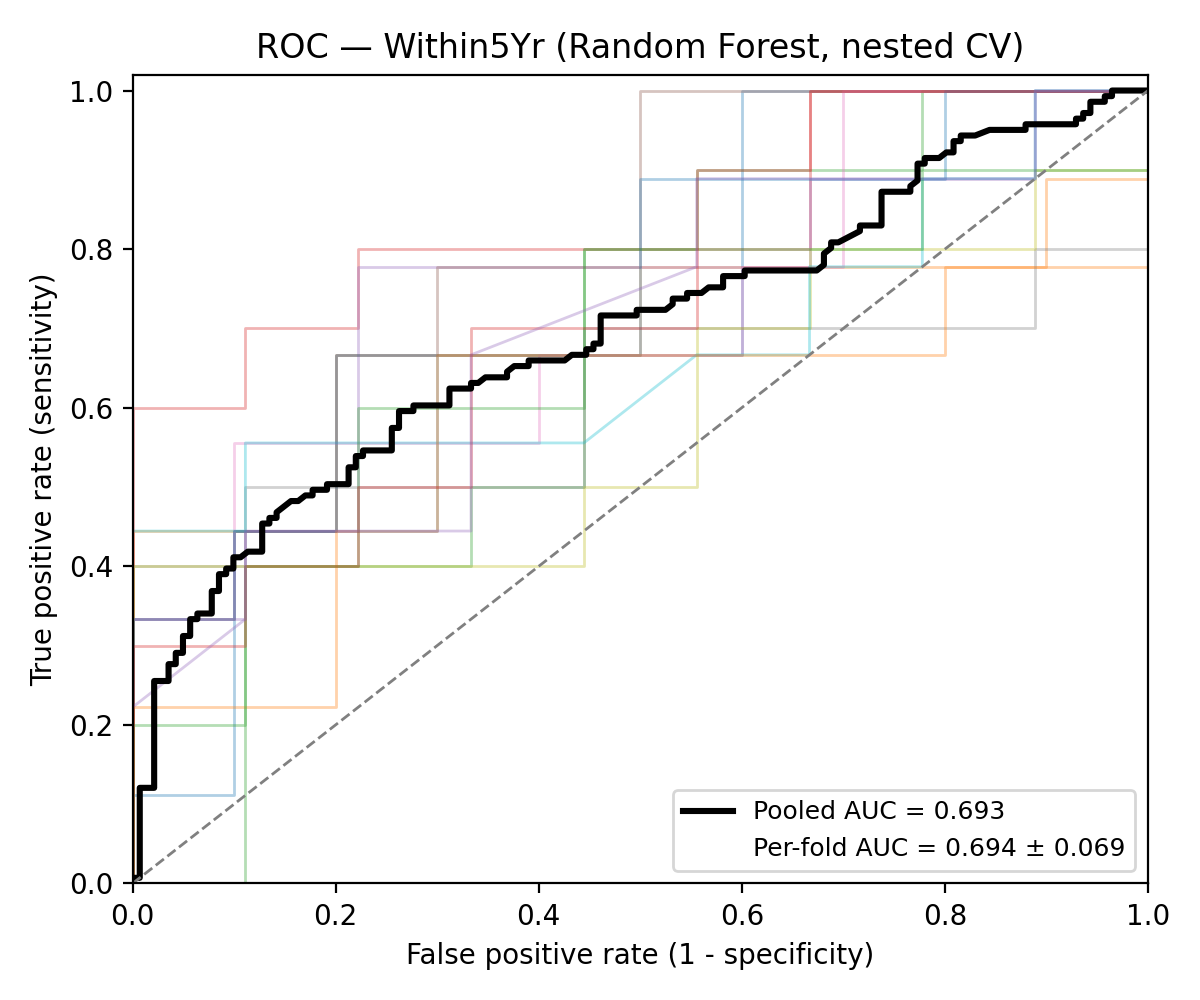
\includegraphics[width=\linewidth]{main_roc_within5yr.png}
    \caption{Within5Yr.}
  \end{subfigure}
  \begin{subfigure}[t]{0.32\textwidth}
    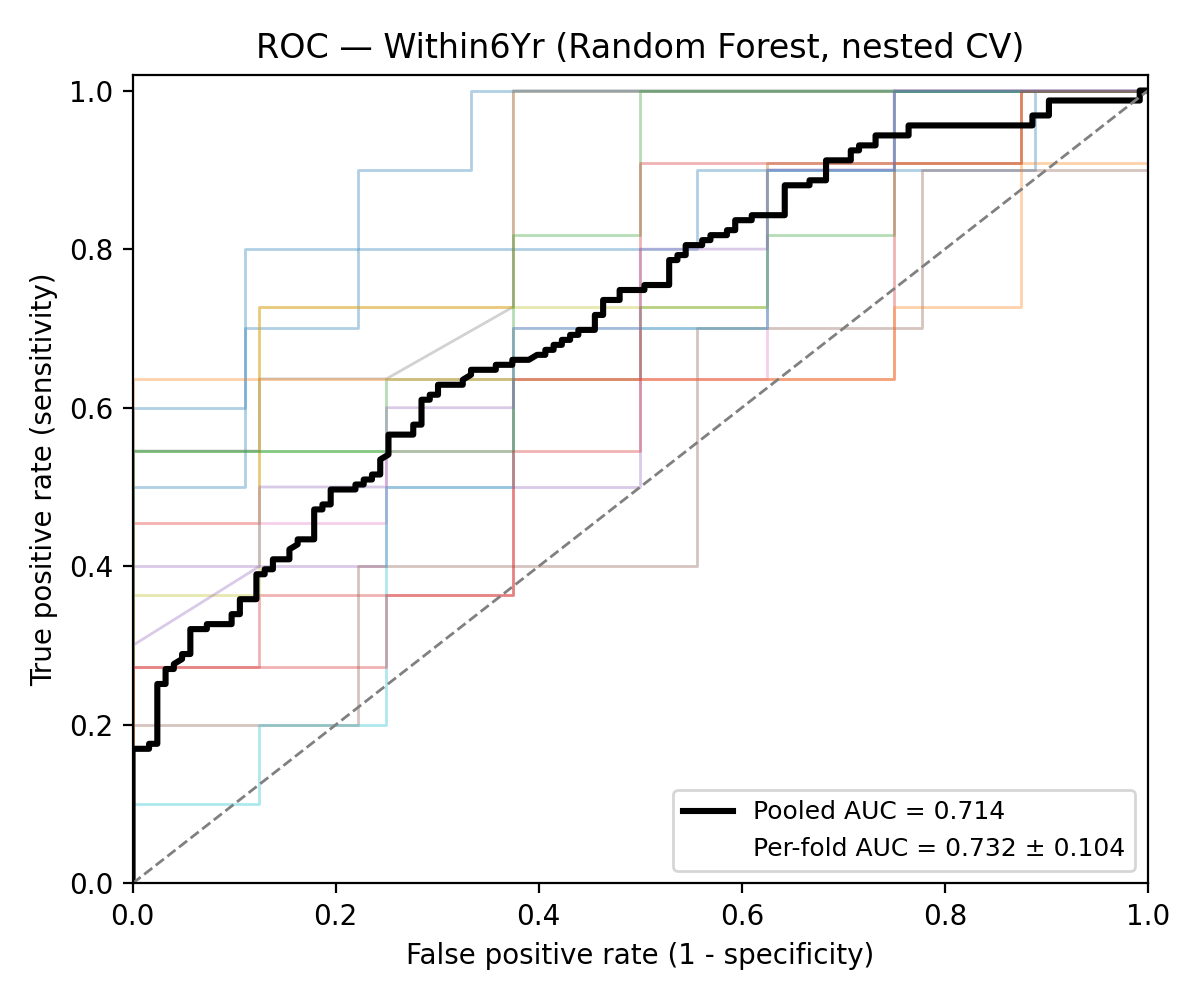
\includegraphics[width=\linewidth]{main_roc_within6yr.png}
    \caption{Within6Yr.}
  \end{subfigure}
  \caption{Per-fold (faint) and pooled (bold) ROC curves for the six
  shorter horizons under nested CV. Within7Yr is shown separately in
  \Cref{fig:within7yr_main}. The pooled-AUC trend climbs monotonically
  from $0.64$ (Within1Yr) to $0.72$ (Within6Yr/Within7Yr).}
  \label{fig:roc_grid}
\end{figure}

\begin{figure}[h]
  \centering
  \begin{subfigure}[t]{0.32\textwidth}
    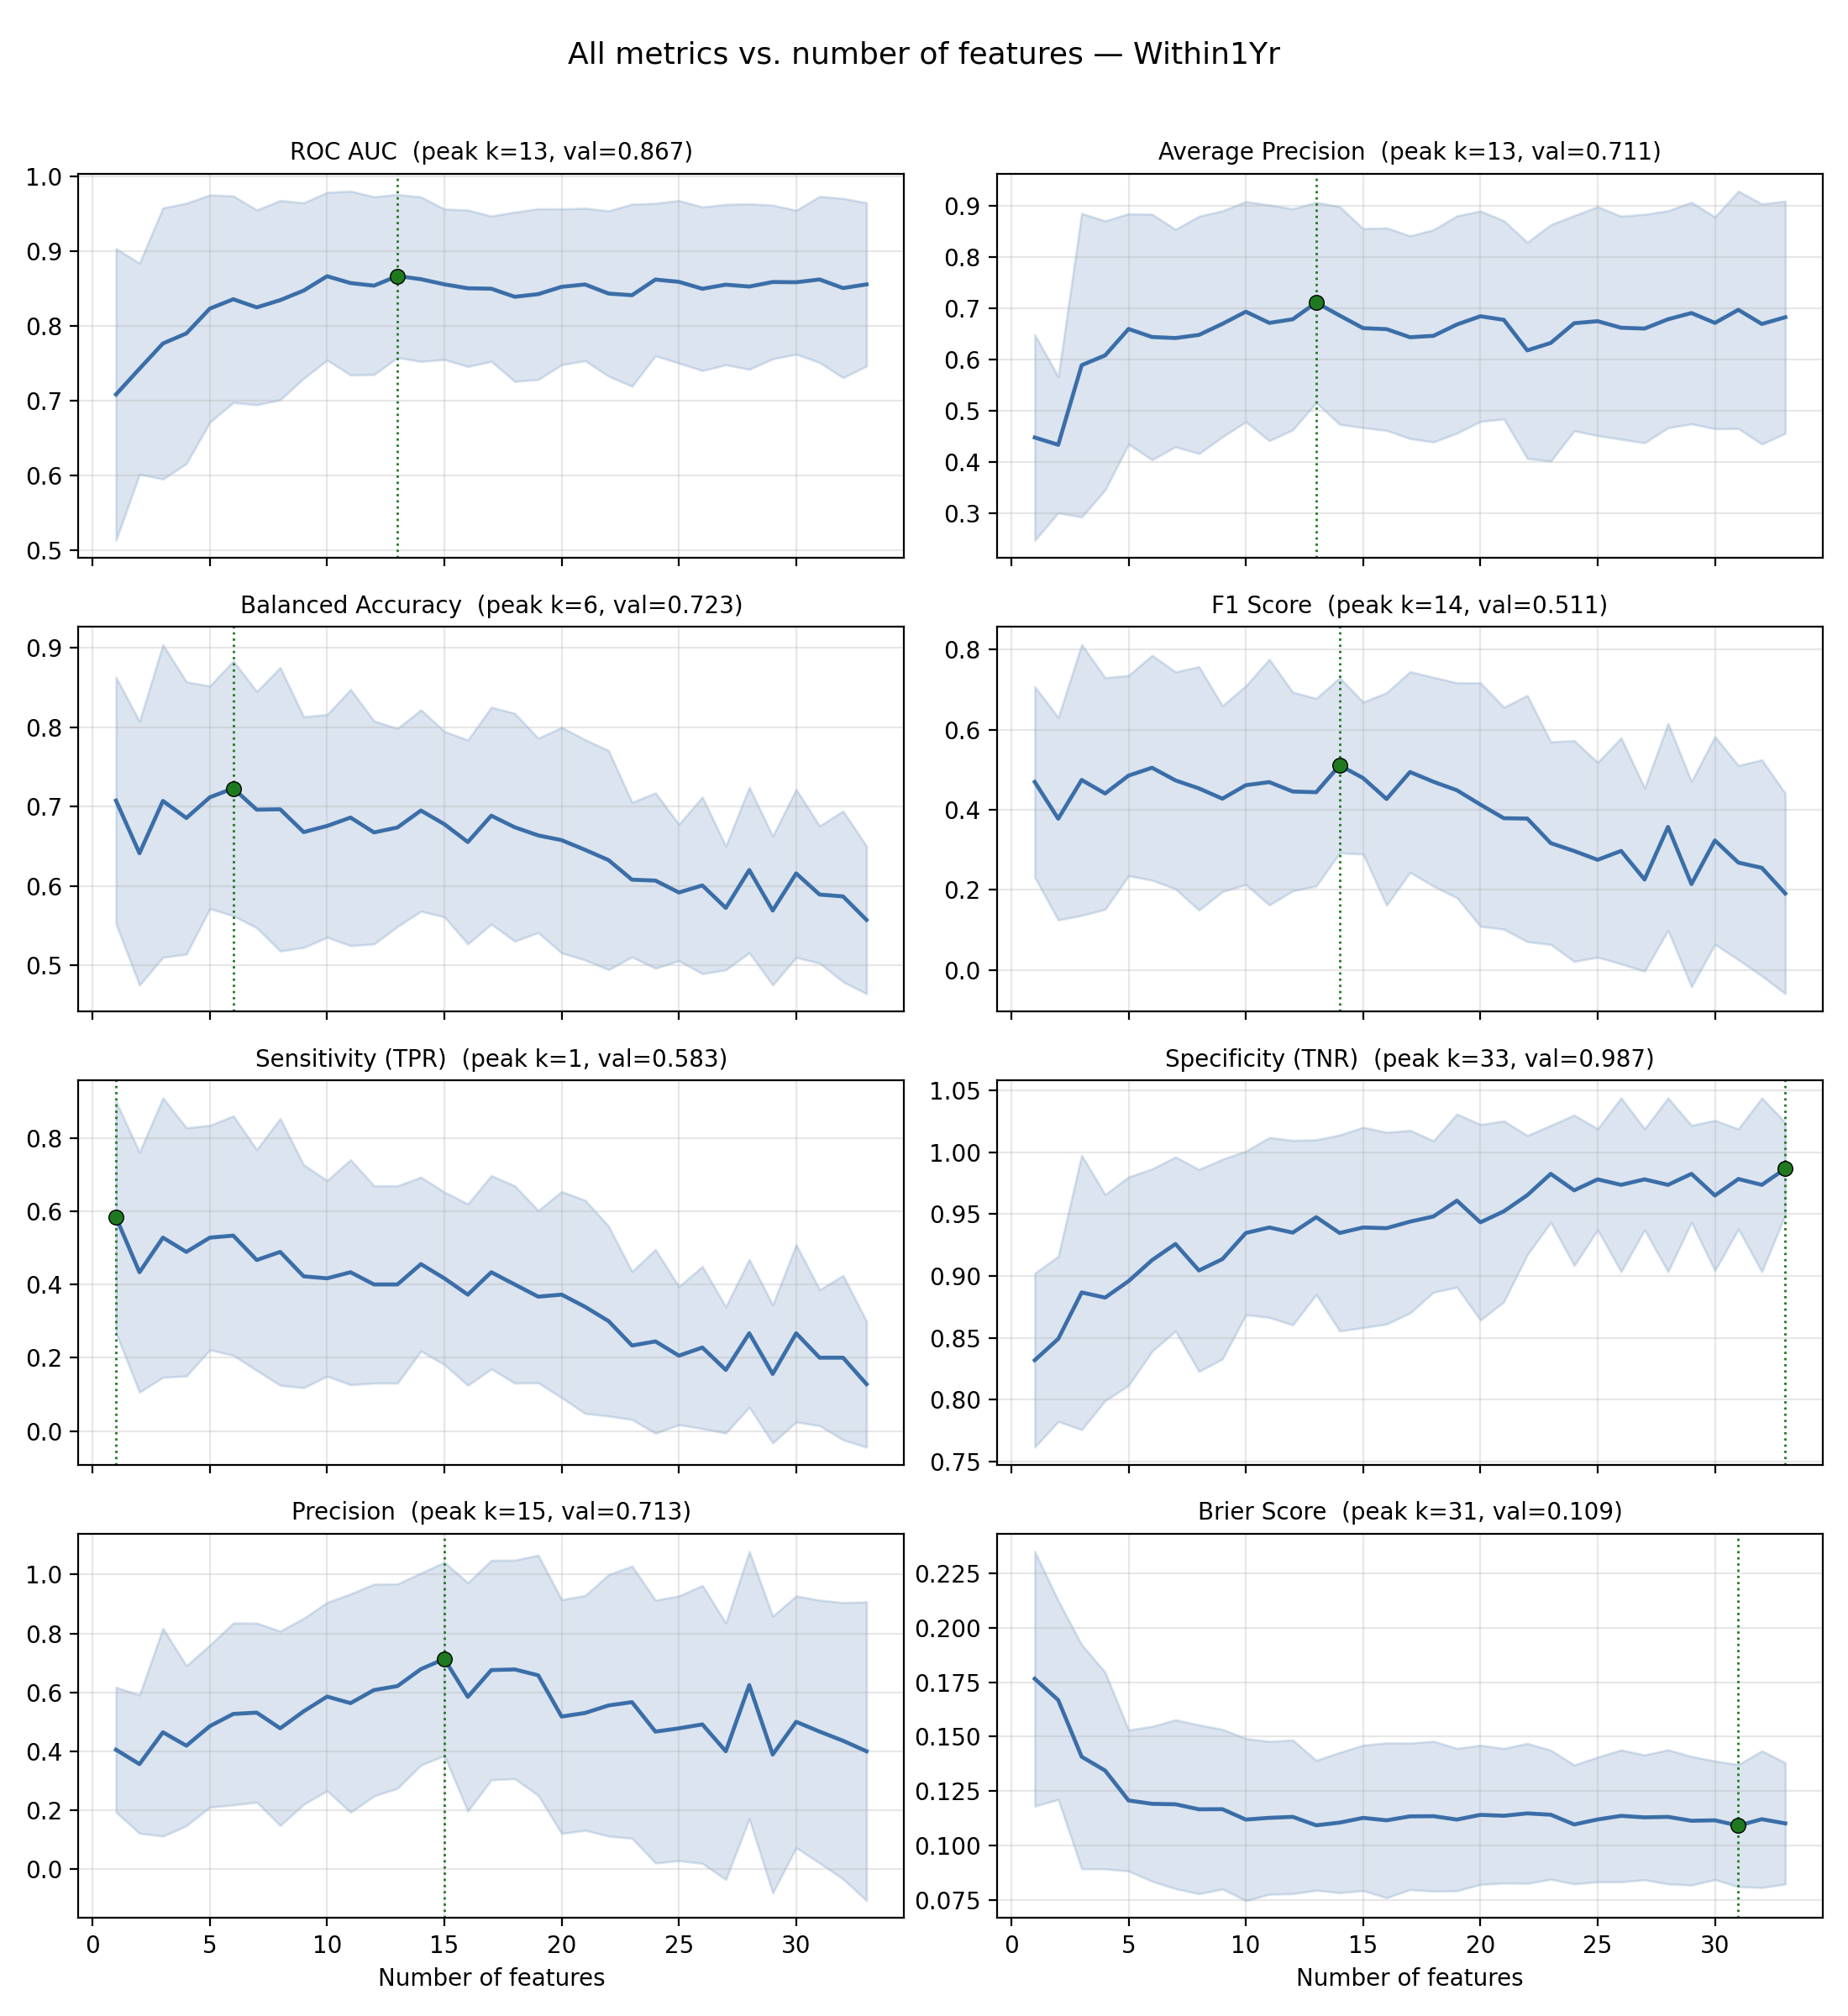
\includegraphics[width=\linewidth]{gradual_allmetrics_within1yr.png}
    \caption{Within1Yr.}
  \end{subfigure}
  \begin{subfigure}[t]{0.32\textwidth}
    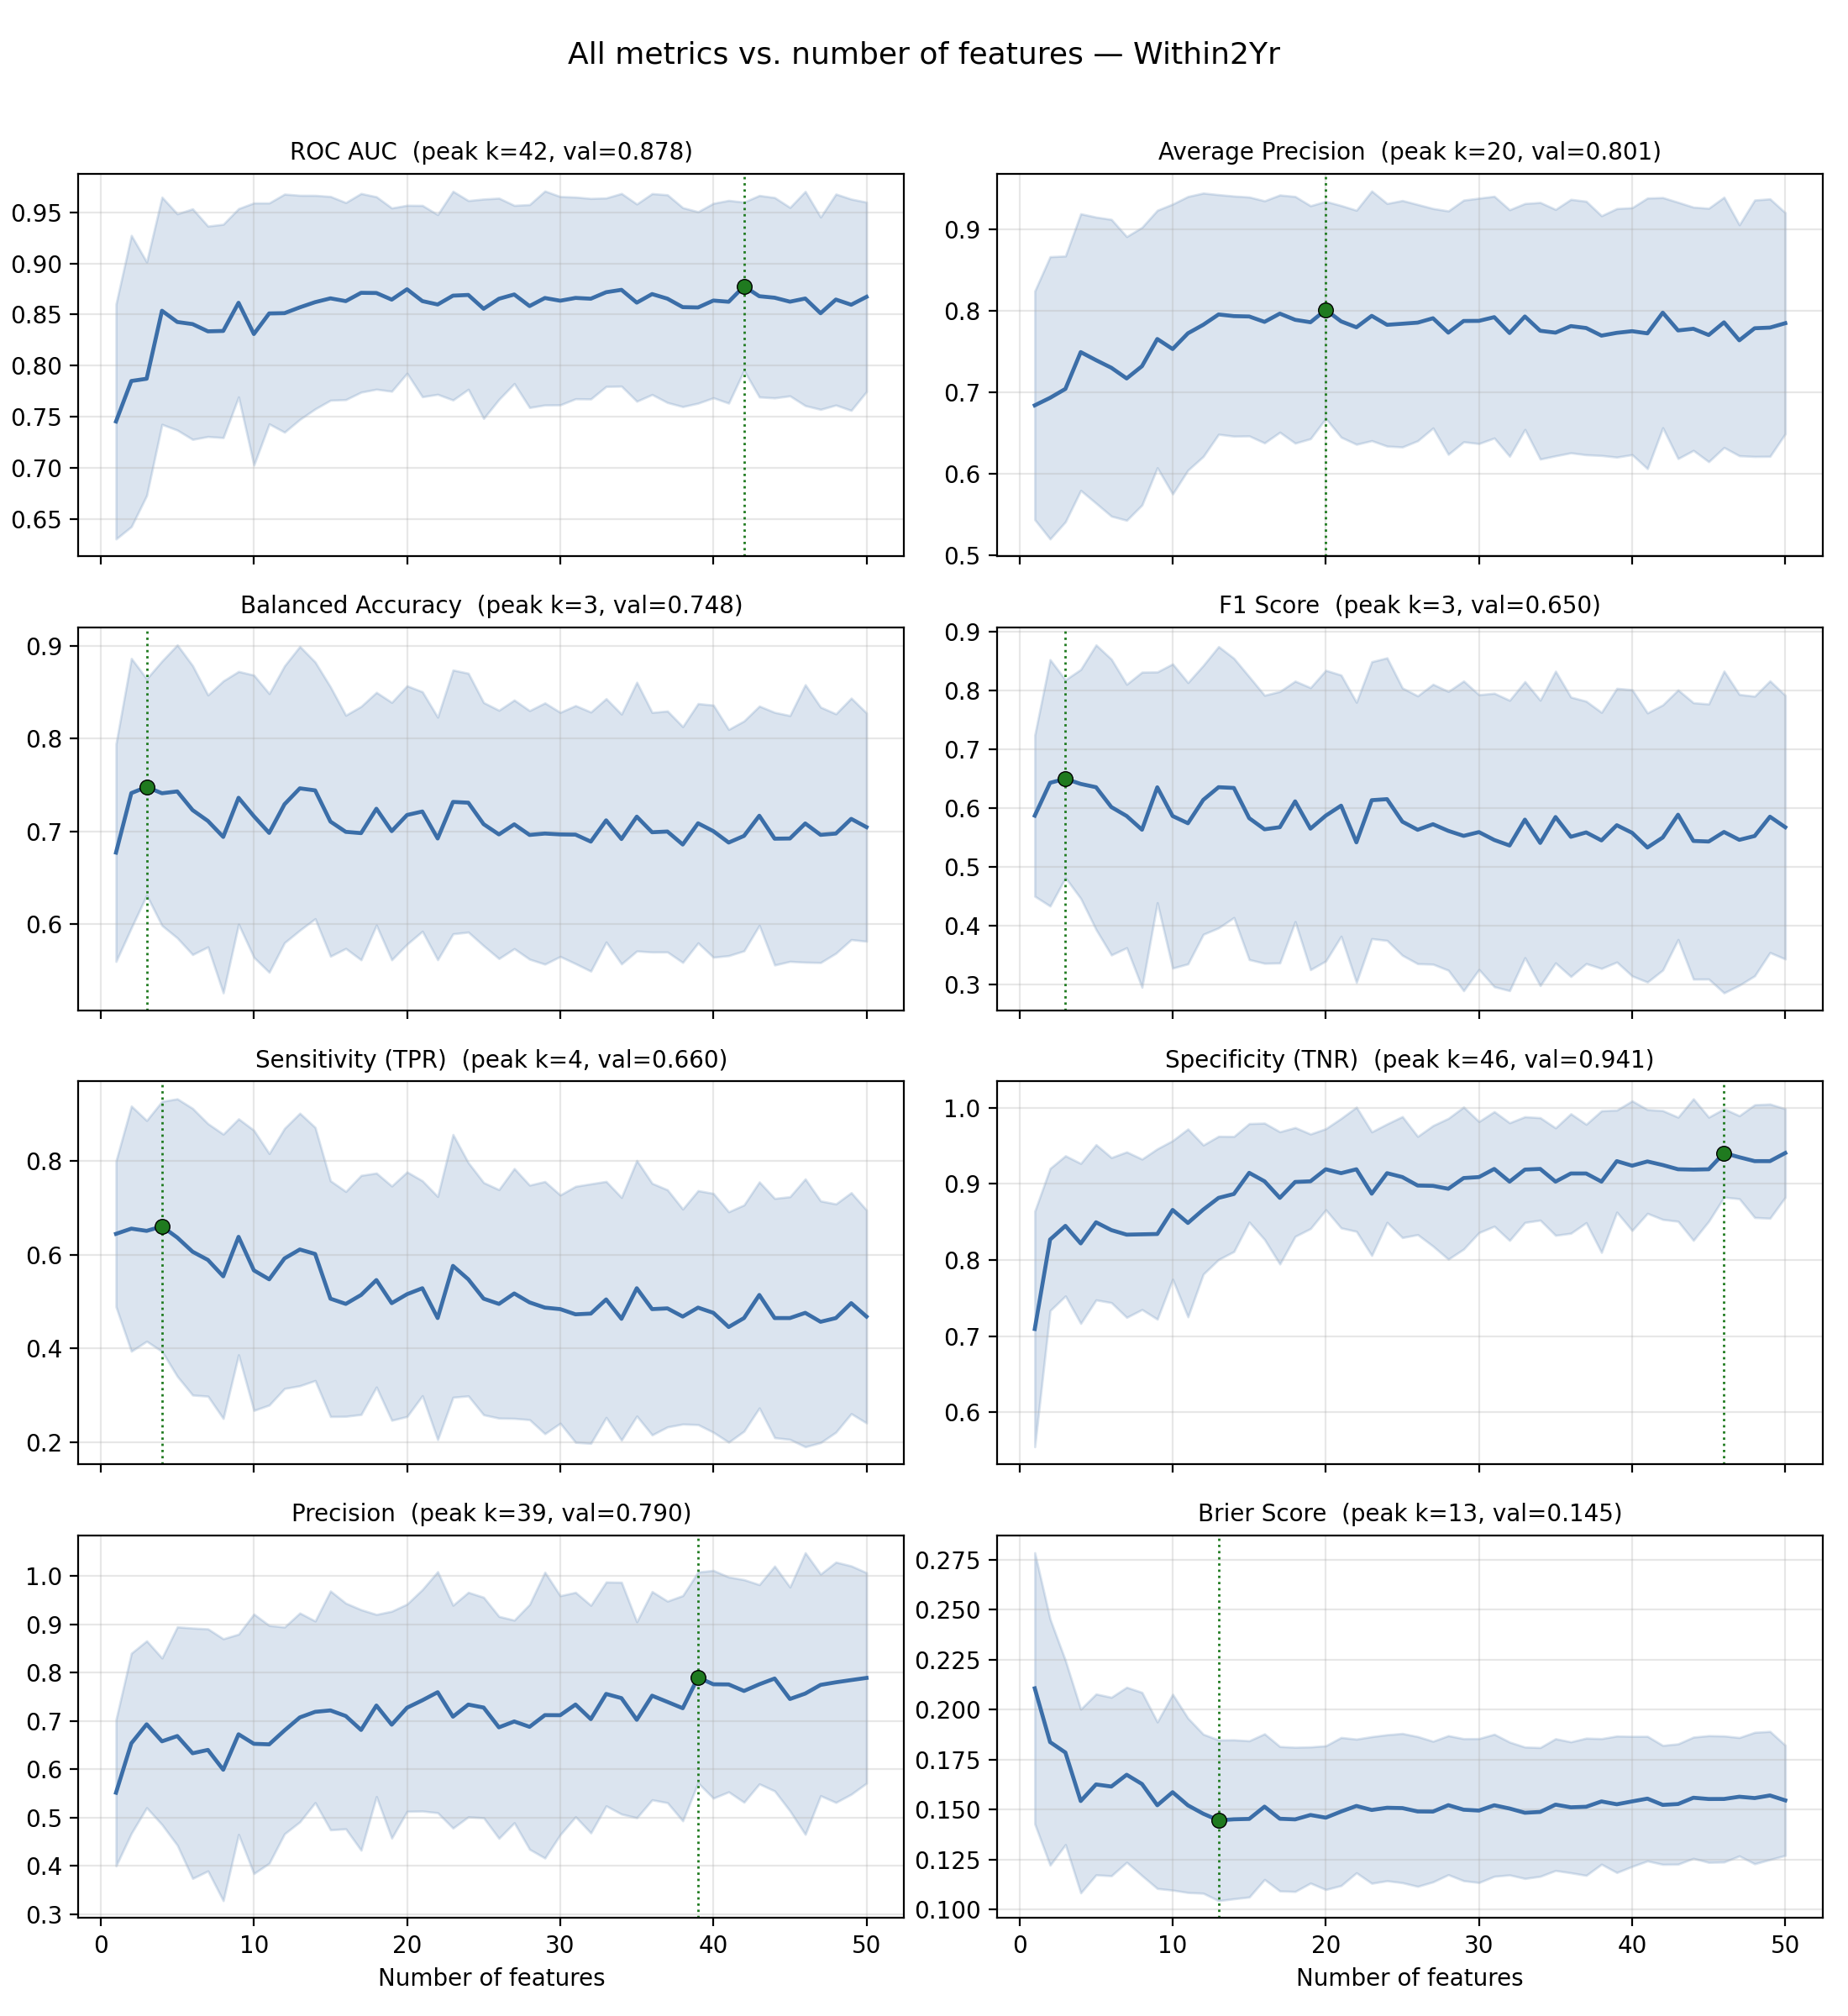
\includegraphics[width=\linewidth]{gradual_allmetrics_within2yr.png}
    \caption{Within2Yr.}
  \end{subfigure}
  \begin{subfigure}[t]{0.32\textwidth}
    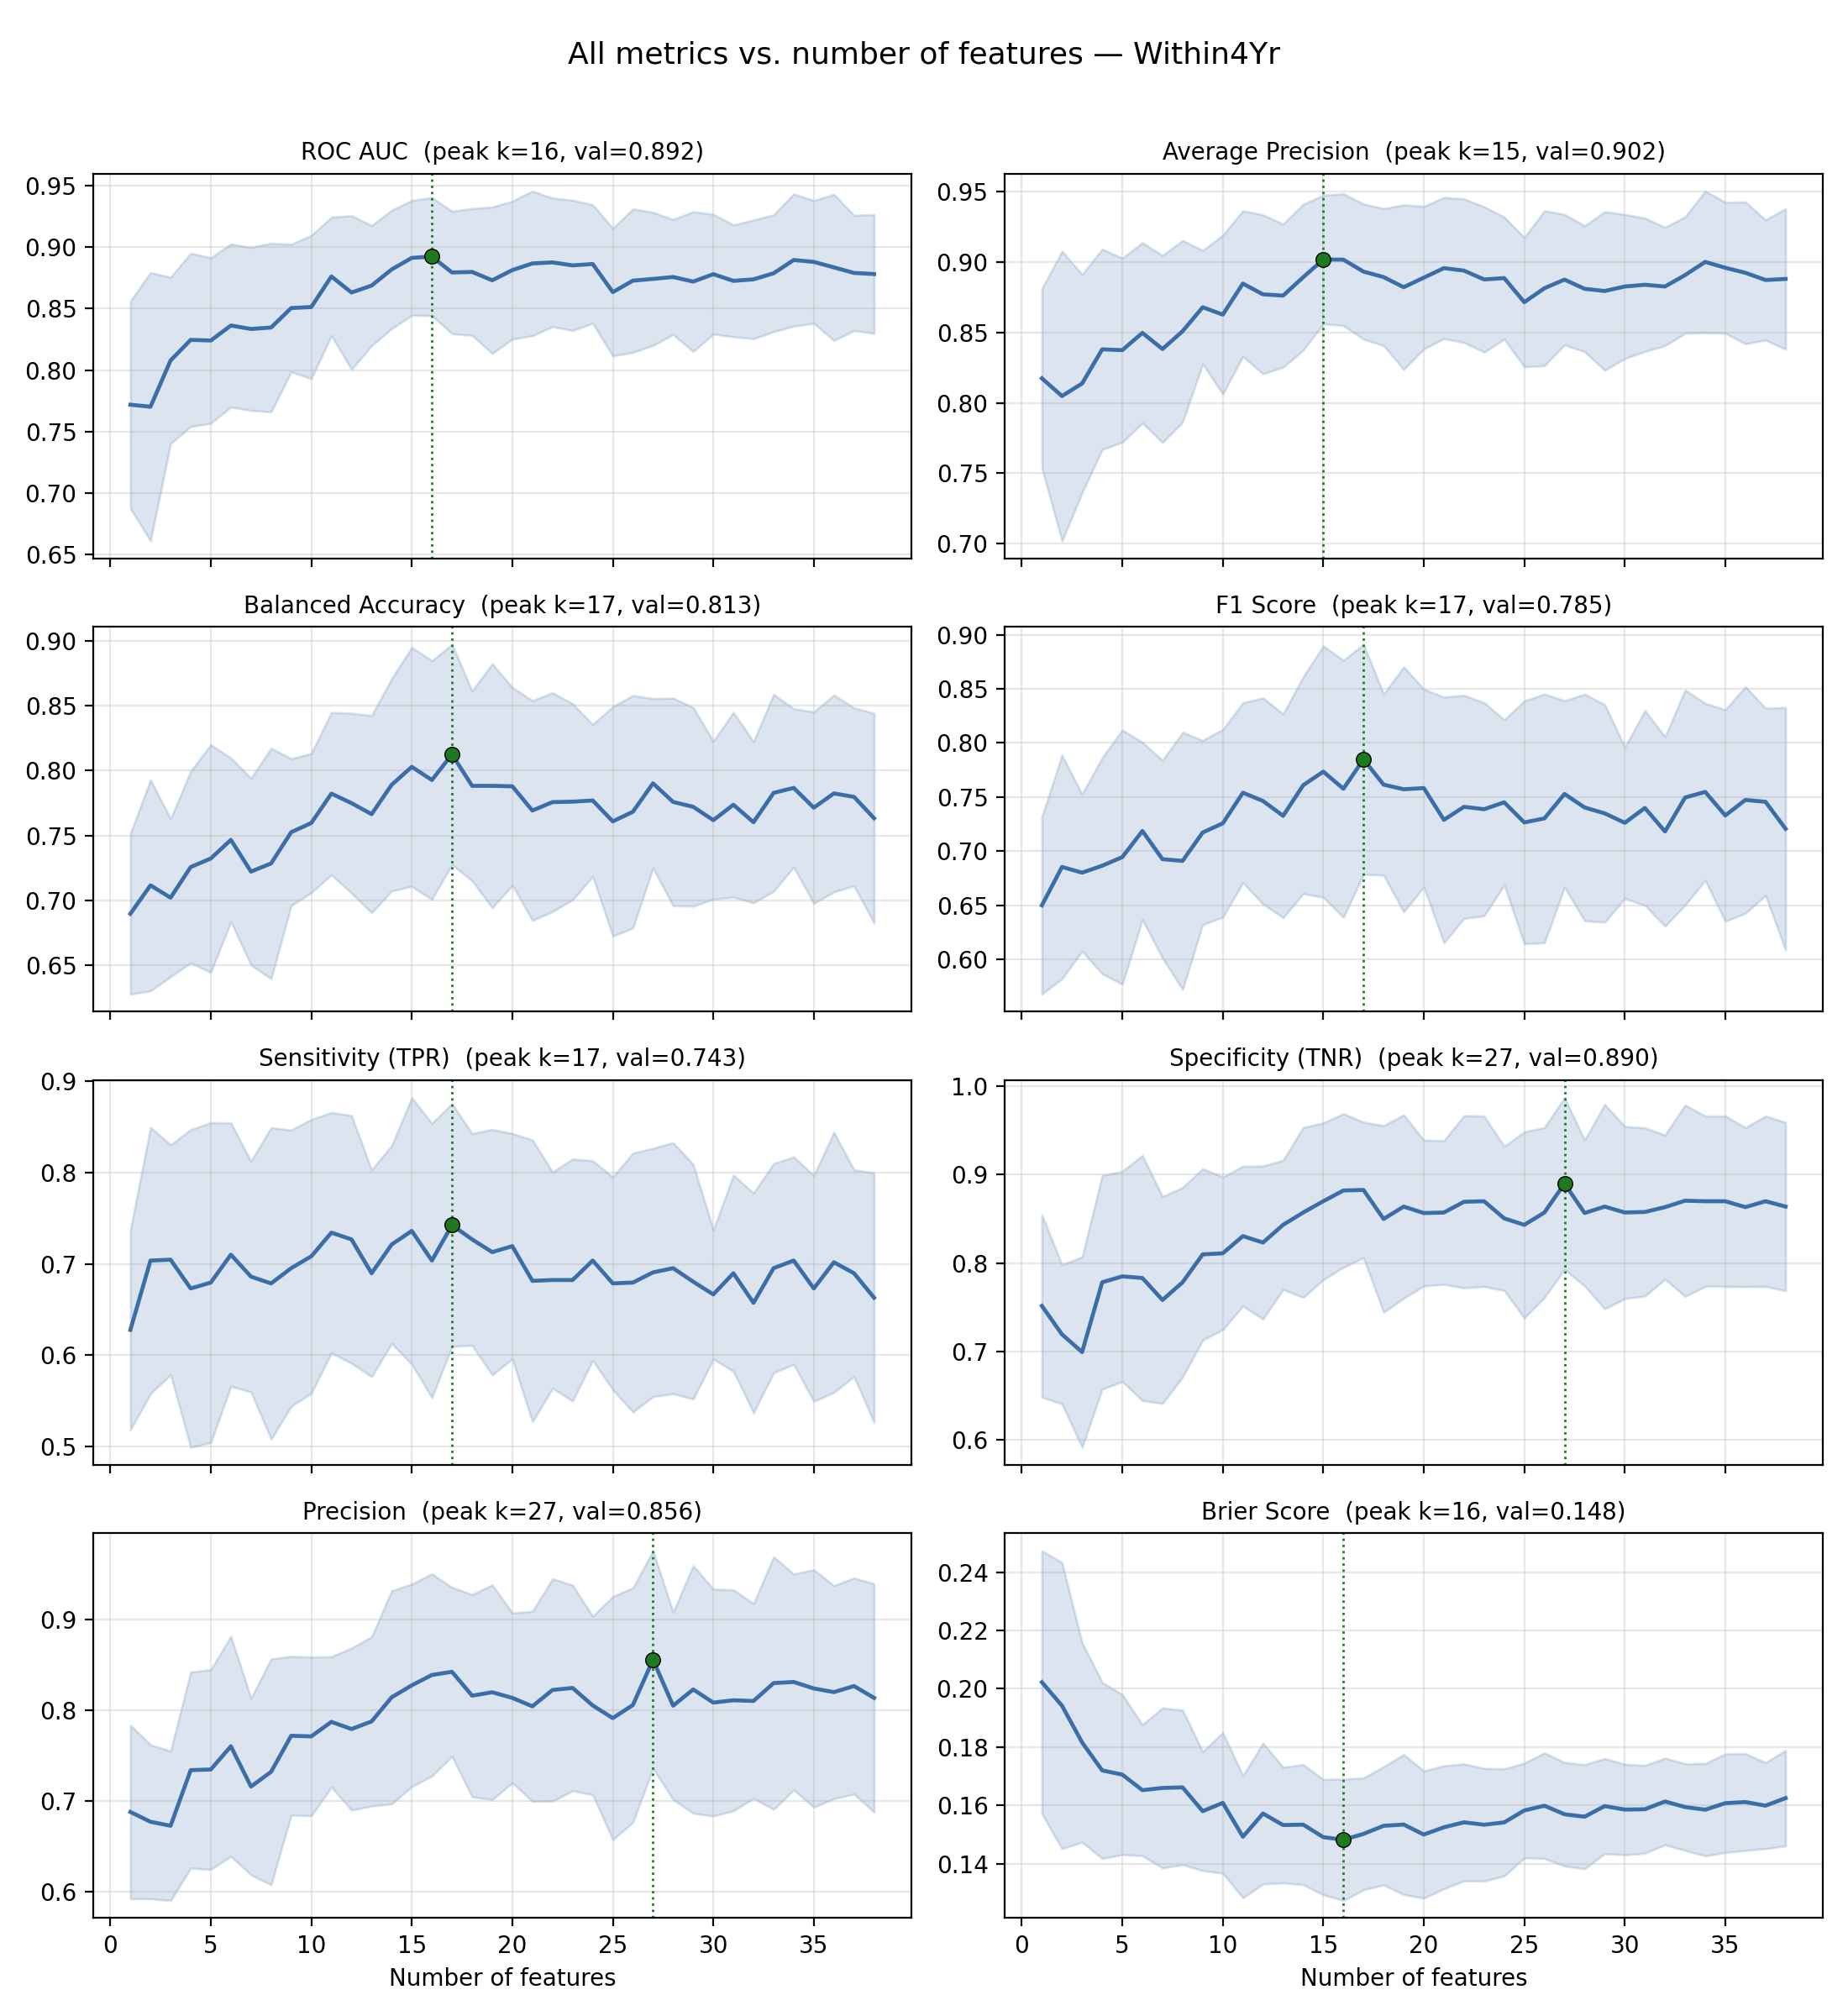
\includegraphics[width=\linewidth]{gradual_allmetrics_within4yr.png}
    \caption{Within4Yr.}
  \end{subfigure}\\
  \begin{subfigure}[t]{0.32\textwidth}
    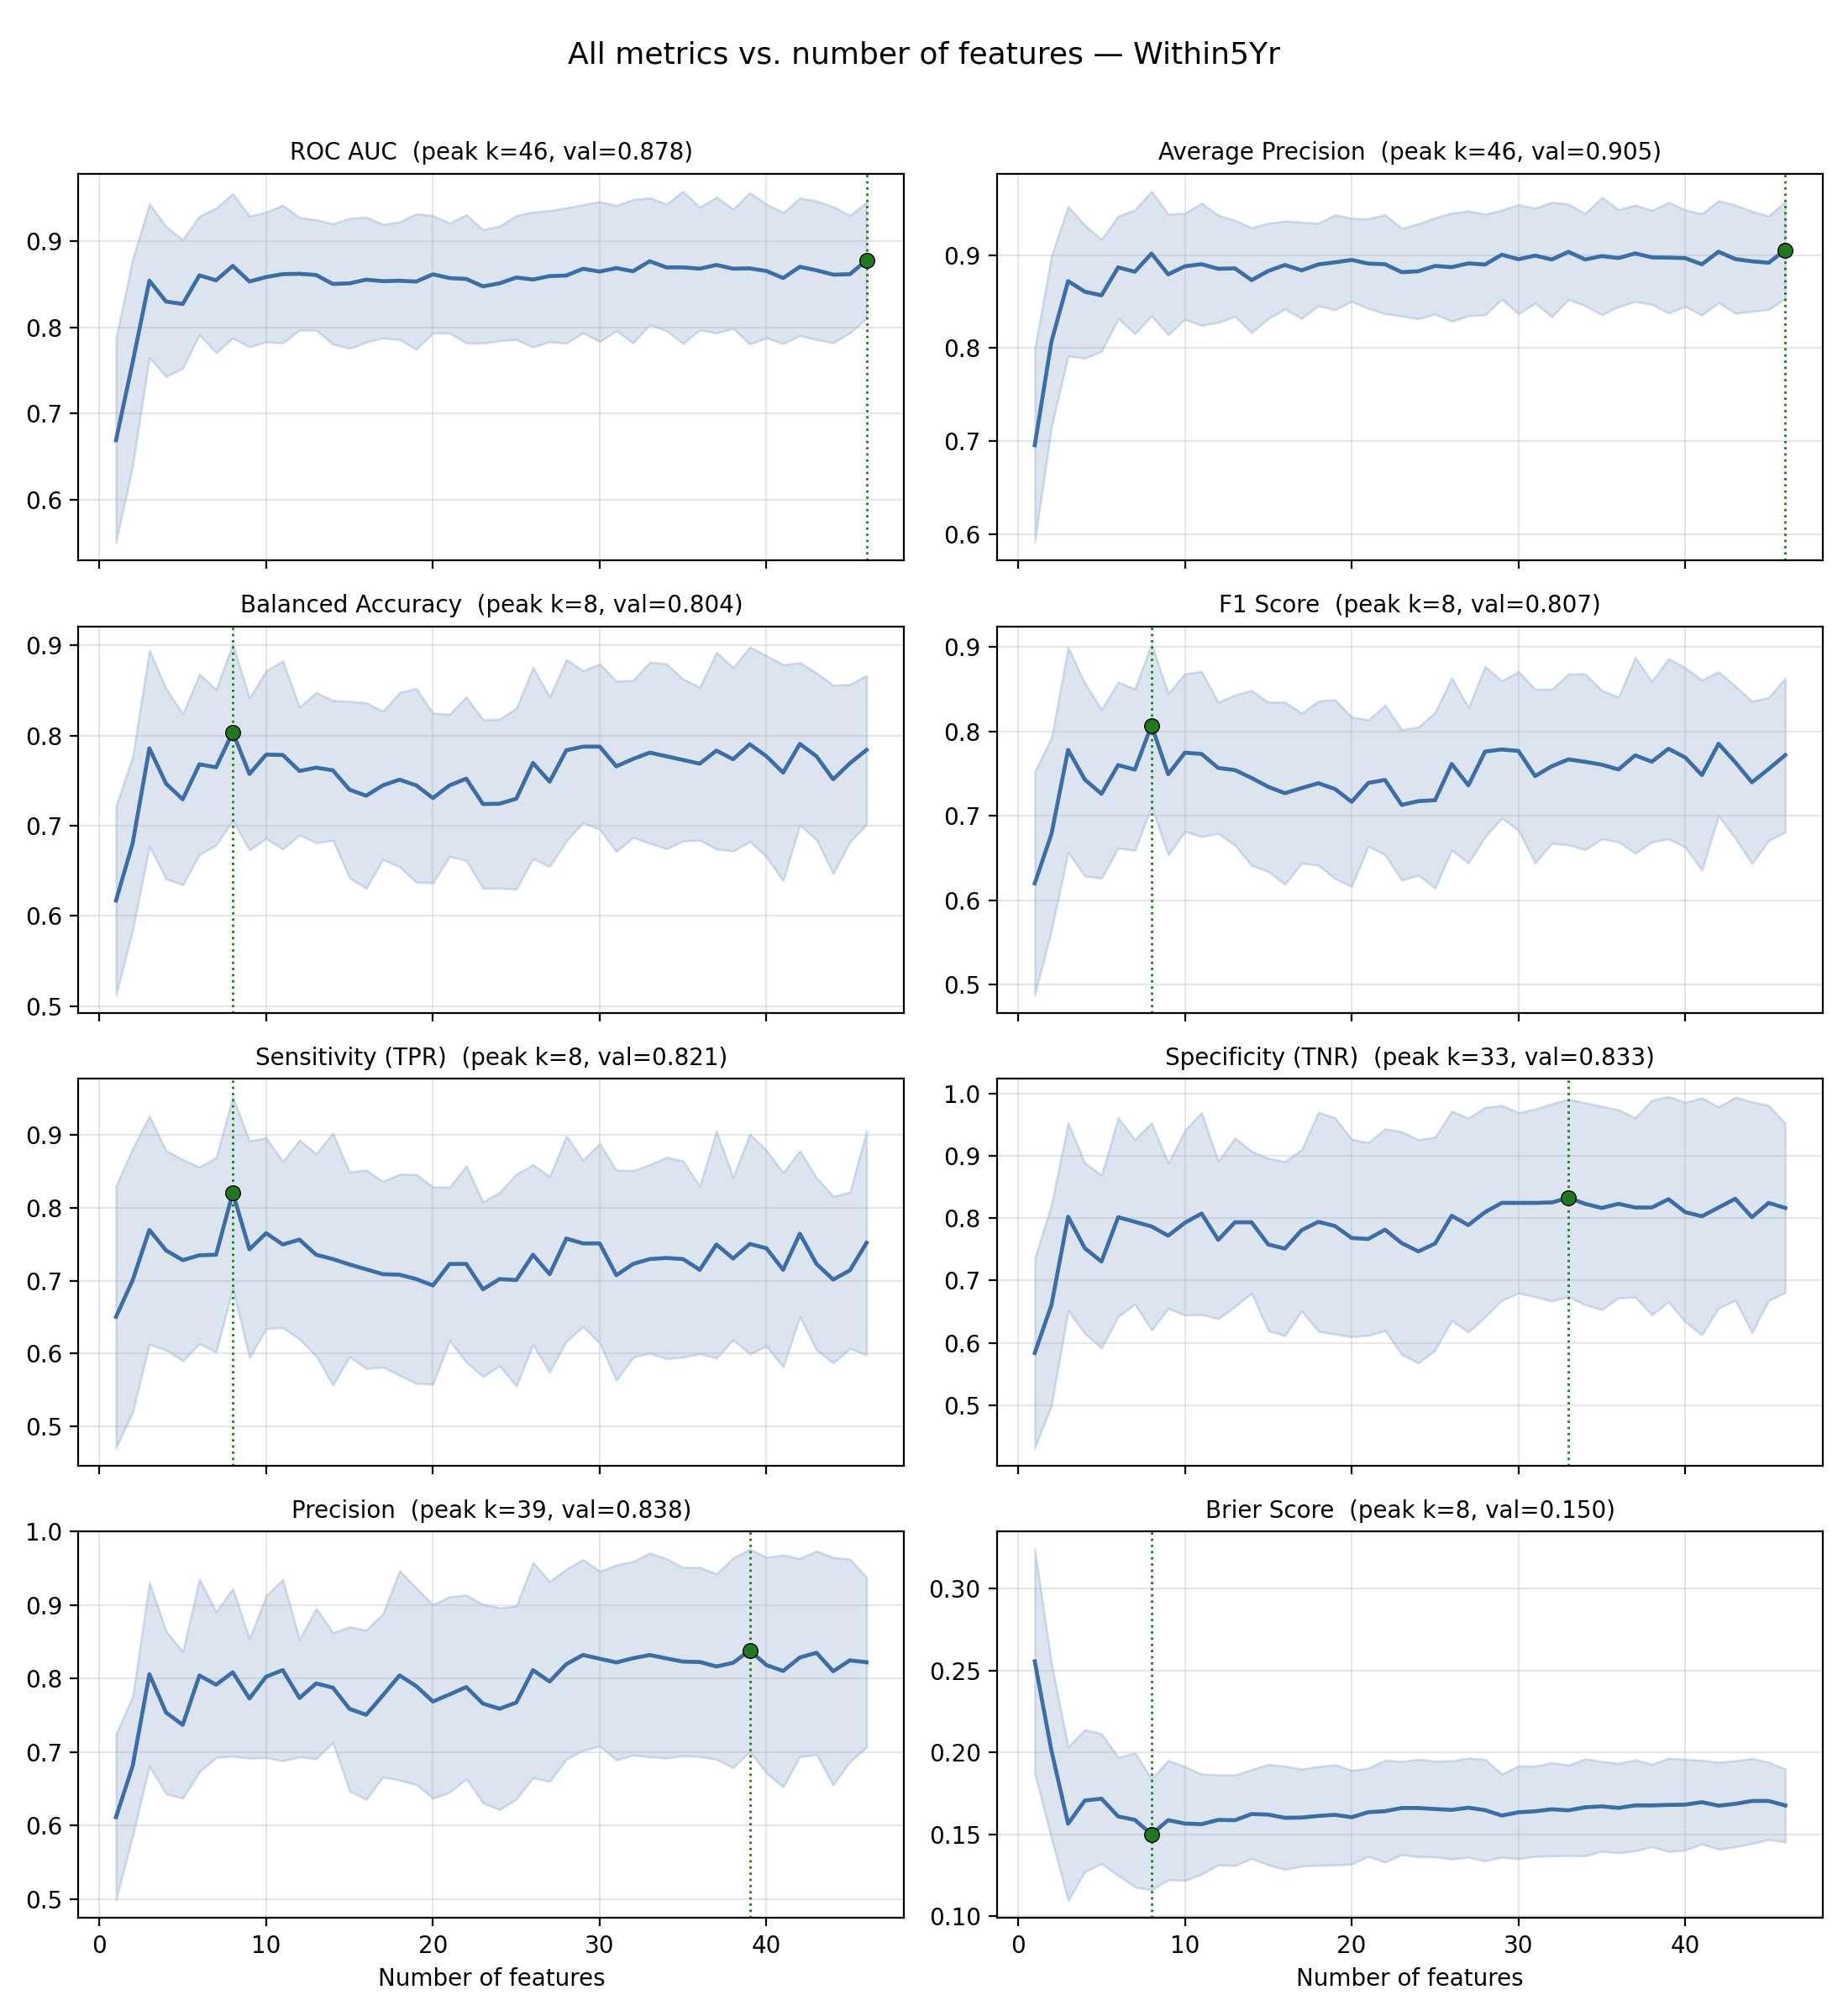
\includegraphics[width=\linewidth]{gradual_allmetrics_within5yr.png}
    \caption{Within5Yr.}
  \end{subfigure}
  \begin{subfigure}[t]{0.32\textwidth}
    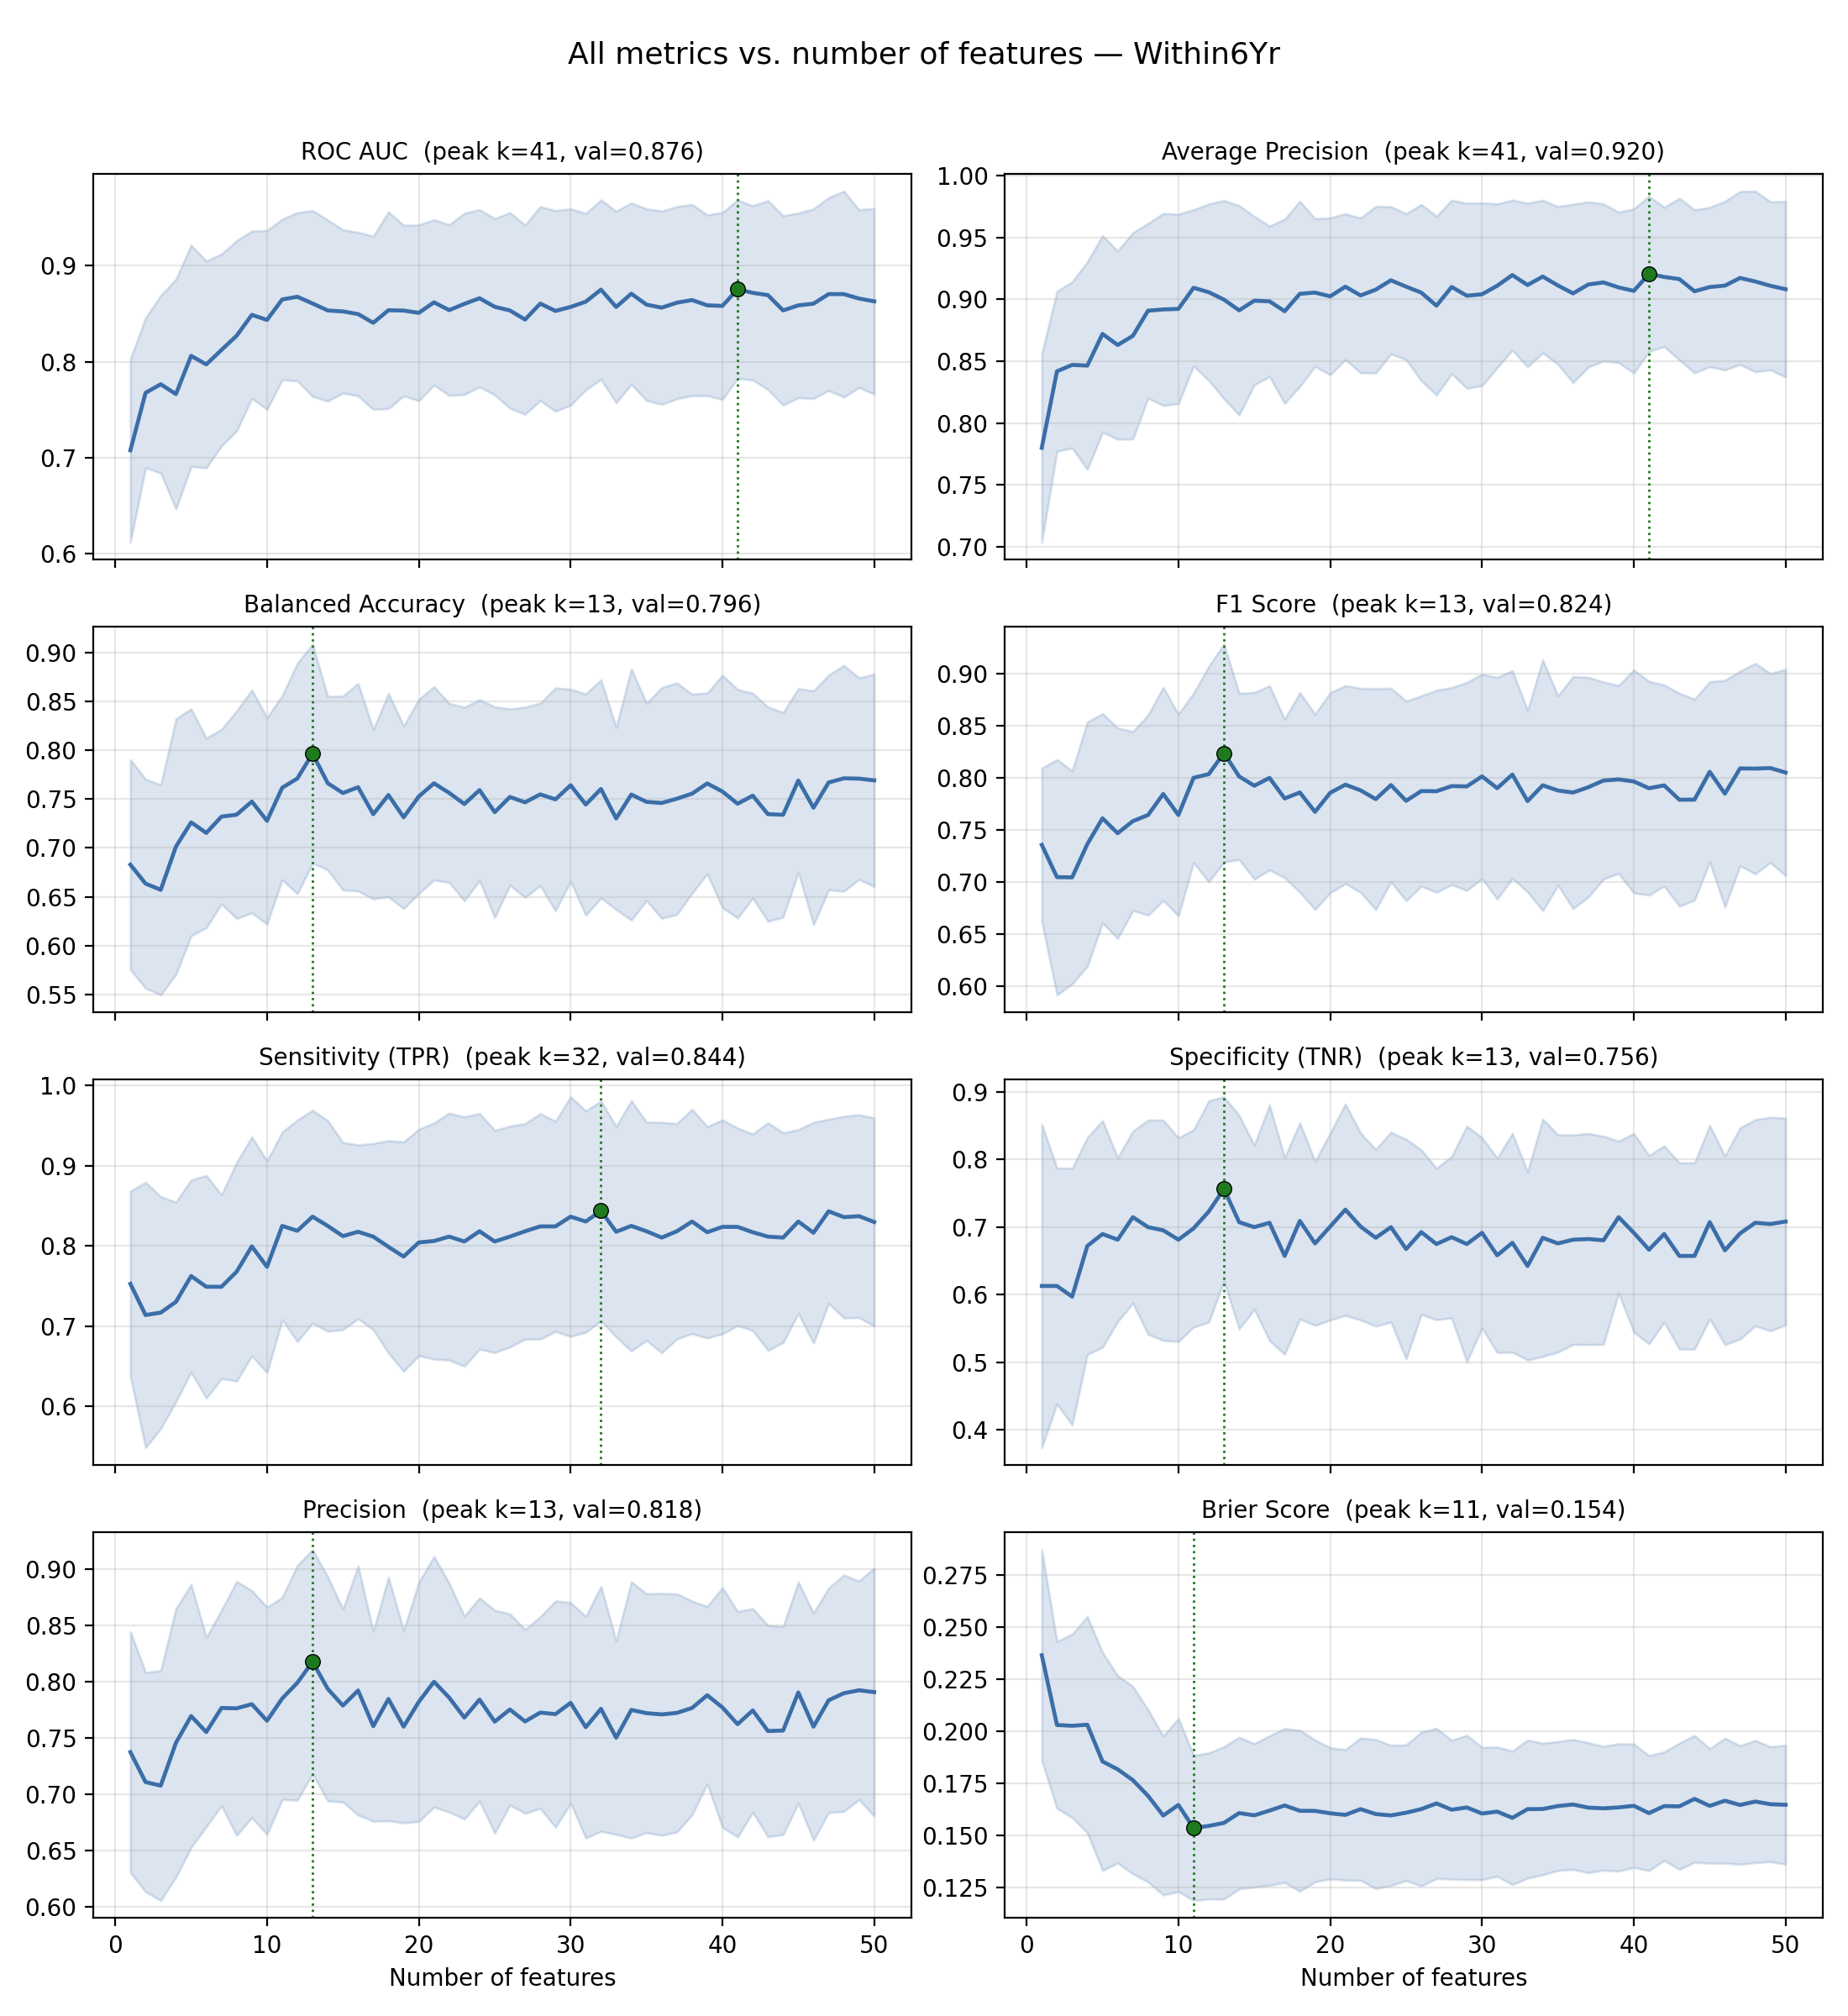
\includegraphics[width=\linewidth]{gradual_allmetrics_within6yr.png}
    \caption{Within6Yr.}
  \end{subfigure}
  \begin{subfigure}[t]{0.32\textwidth}
    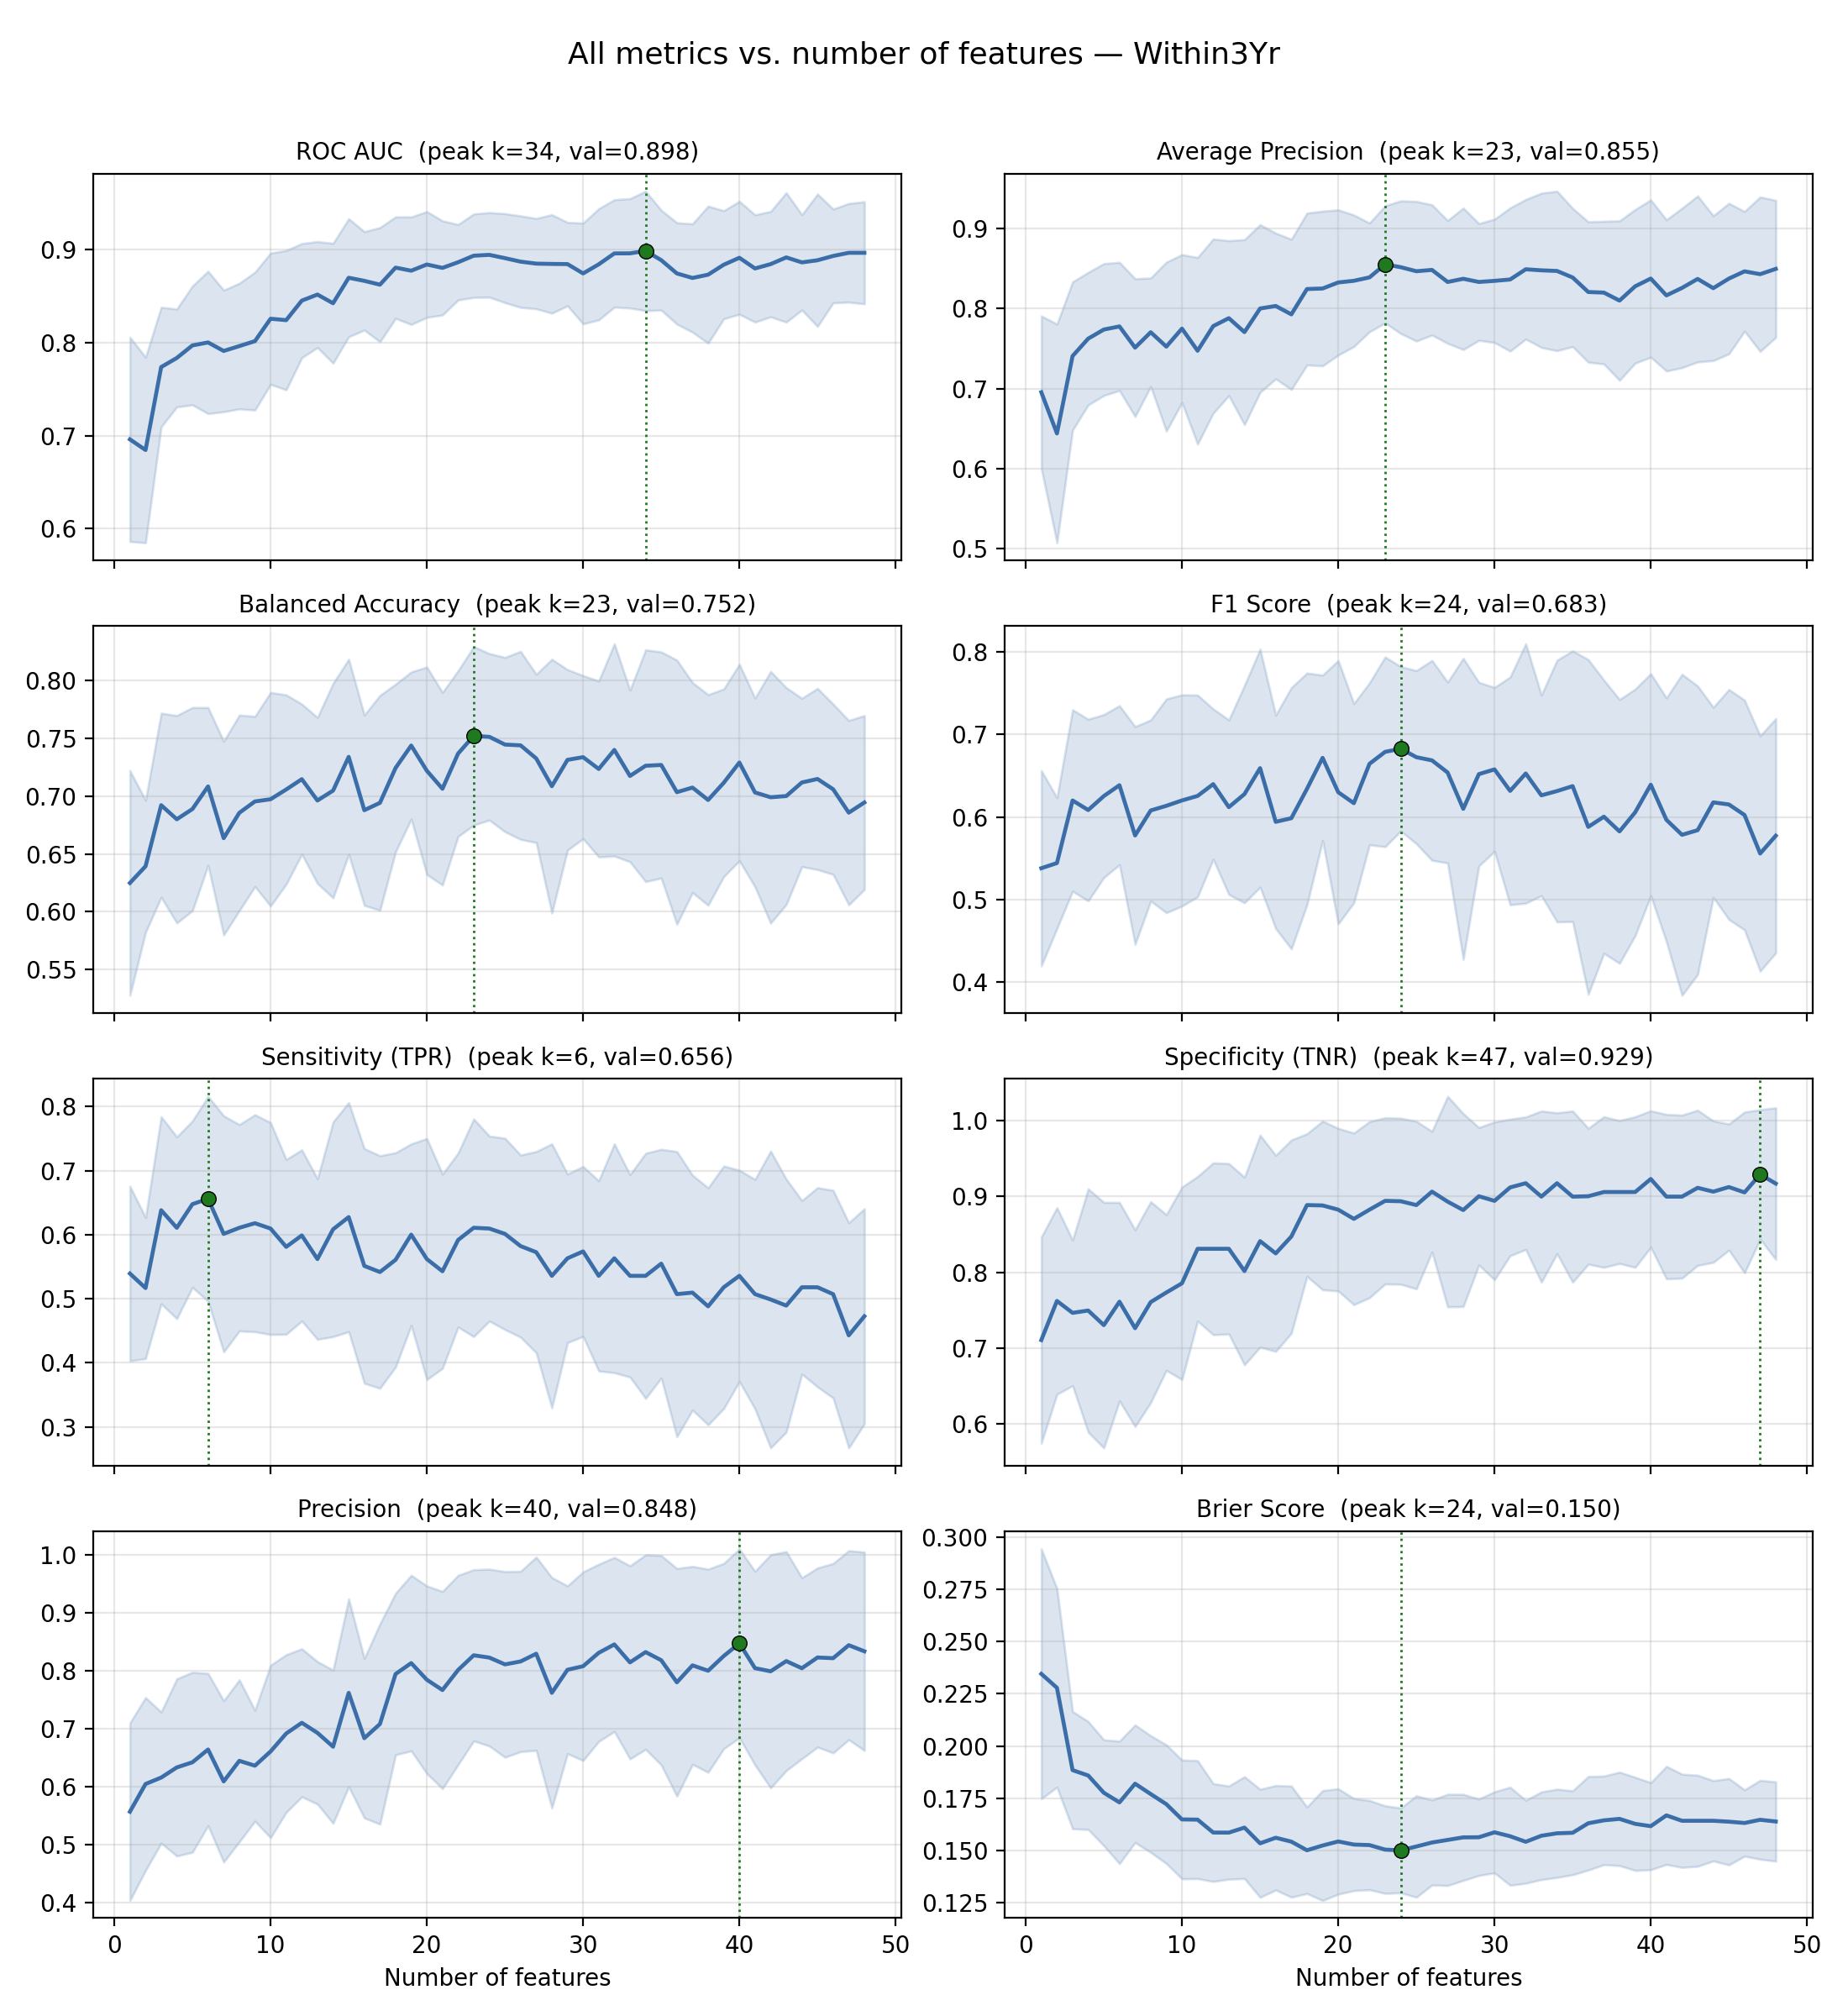
\includegraphics[width=\linewidth]{gradual_allmetrics_within3yr.png}
    \caption{Within3Yr.}
  \end{subfigure}
  \caption{Gradual-training all-metric panels for the six non-headline
  horizons. Each panel shows ten metrics versus feature count $k$;
  Within7Yr is in \Cref{fig:within7yr_gradual_all}. The shape ``sharp
  early gain, then plateau'' repeats across all horizons, which is the
  central parsimony observation of the project.}
  \label{fig:gradual_grid}
\end{figure}

\subsection{Headline horizon: Within7Yr walkthrough}
\label{sec:within7yr}

We anchor the headline narrative on \textbf{Within7Yr} for three
reasons: (i) it is the most class-balanced horizon ($56/94 = 60\%$
positives; \Cref{fig:survival}), so accuracy and balanced-accuracy
metrics are most informative; (ii) it offers the longest follow-up,
which is the clinical scenario most relevant to long-term risk
stratification; and (iii) it produced the strongest results across the
pipeline (Tables~\ref{tab:headline} and~\ref{tab:gradual_summary}). All
of the artefacts shown below are produced by the same pipeline and the
same fixed seed as the rest of the paper.

\subsubsection*{Pooled discrimination.}
Pooled out-of-fold ROC-AUC is $0.719$ and per-fold mean ROC-AUC is
$0.735\pm 0.089$ (\Cref{fig:within7yr_main}, panel a). Pooled
average precision is $0.792$ (\Cref{fig:within7yr_main}, panel b), well
above the prior of $0.60$, indicating that the predicted probabilities
rank events ahead of non-events meaningfully better than the
prevalence baseline. The selected hyperparameters from the inner CV
were \texttt{n\_estimators}$=300$, \texttt{max\_depth}$=$None,
\texttt{min\_samples\_leaf}$=1$, \texttt{max\_features}$=\sqrt{p}$, with
final stability selection retaining $|\mathcal{F}|=49$ features.

\begin{figure}[h]
  \centering
  \begin{subfigure}[t]{0.48\textwidth}
    \centering
    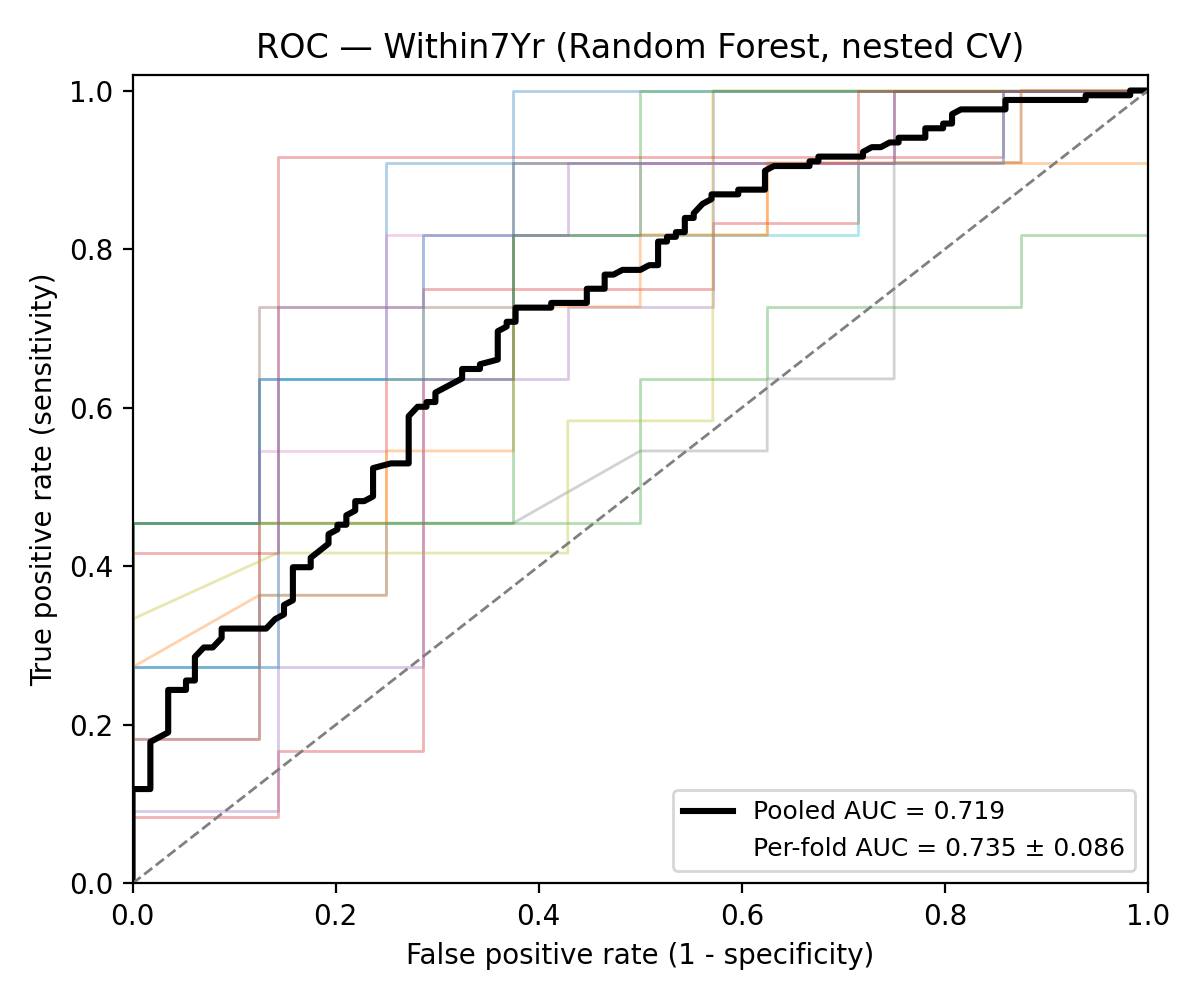
\includegraphics[width=\linewidth]{main_roc_within7yr.png}
    \caption{Per-fold and pooled ROC.}
  \end{subfigure}
  \hfill
  \begin{subfigure}[t]{0.48\textwidth}
    \centering
    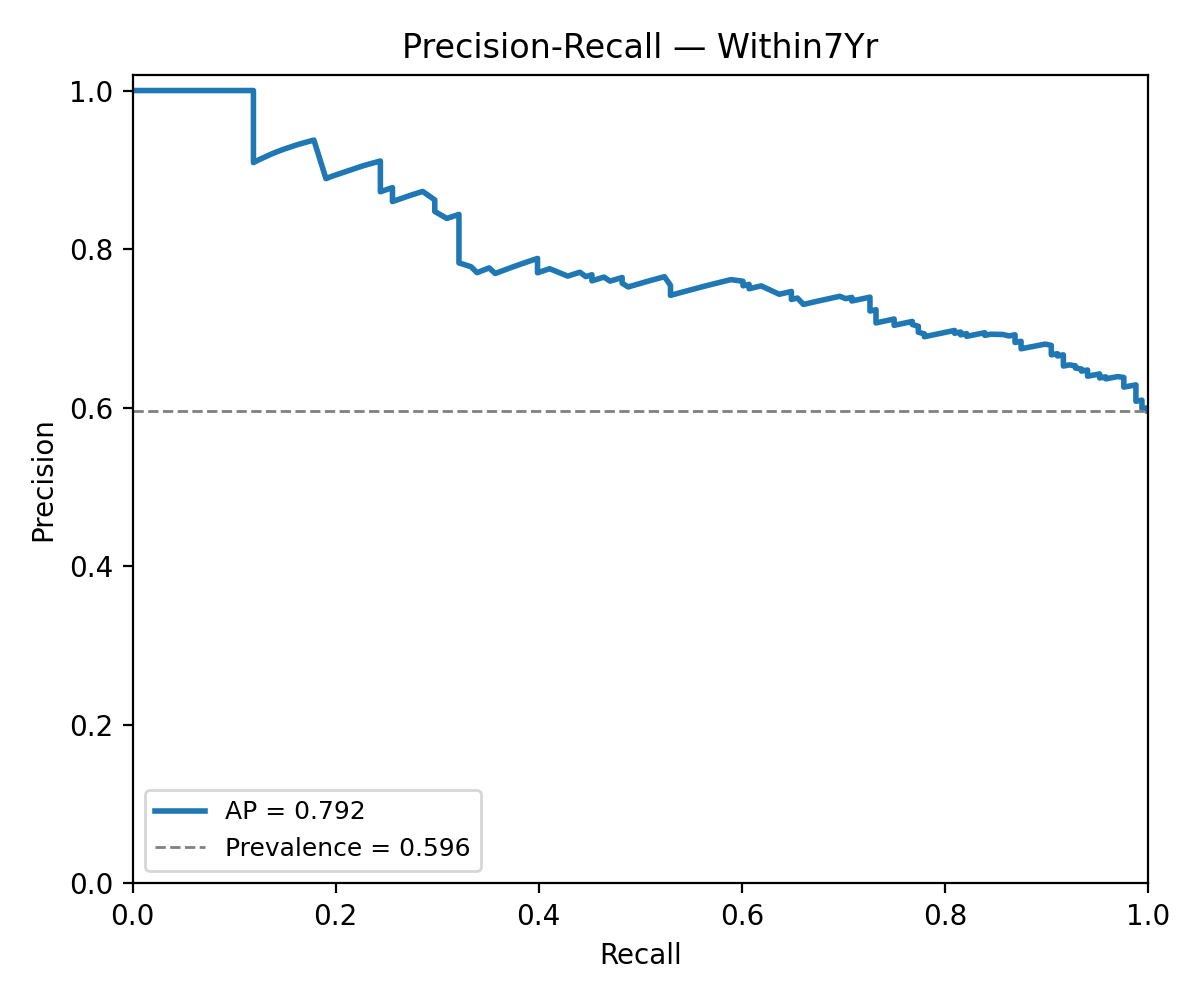
\includegraphics[width=\linewidth]{main_pr_within7yr.png}
    \caption{Pooled precision-recall.}
  \end{subfigure}
  \caption{Within7Yr held-out discrimination under nested CV. Faint
  curves are the $15$ outer folds; the bold curve is computed from the
  concatenated out-of-fold probabilities. The marked operating point in
  (a) is the Youden-optimal threshold $\tau^\star = 0.58$.}
  \label{fig:within7yr_main}
\end{figure}

\subsubsection*{Operating points and confusion structure.}
Two thresholds are reported (\Cref{fig:within7yr_cm}). At
$\tau=0.50$ the model achieves sensitivity $0.81$ and specificity
$0.48$: it correctly flags four out of five future MACE patients but
makes too many false alarms among the smaller negative group. The
Youden-optimal threshold $\tau^\star=0.58$ rebalances this: sensitivity
$0.73$, specificity $0.62$, balanced accuracy $0.674$. The Youden cut
is the operating point we recommend for any downstream clinical use.

\begin{figure}[h]
  \centering
  \begin{subfigure}[t]{0.48\textwidth}
    \centering
    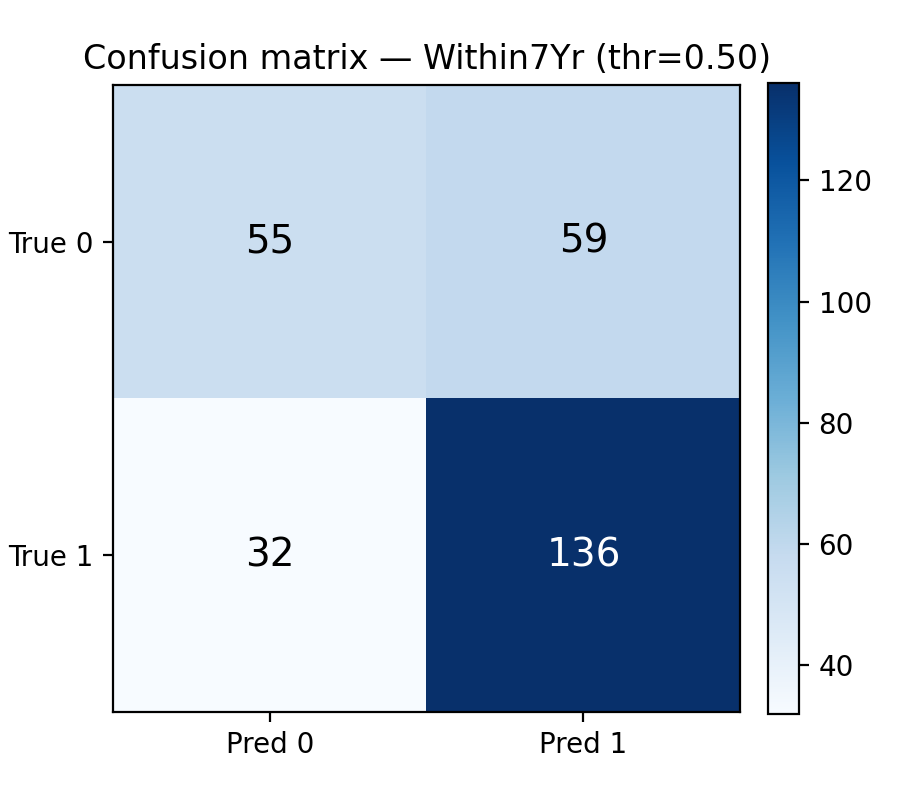
\includegraphics[width=\linewidth]{main_cm05_within7yr.png}
    \caption{Pooled confusion matrix at $\tau=0.50$.}
  \end{subfigure}
  \hfill
  \begin{subfigure}[t]{0.48\textwidth}
    \centering
    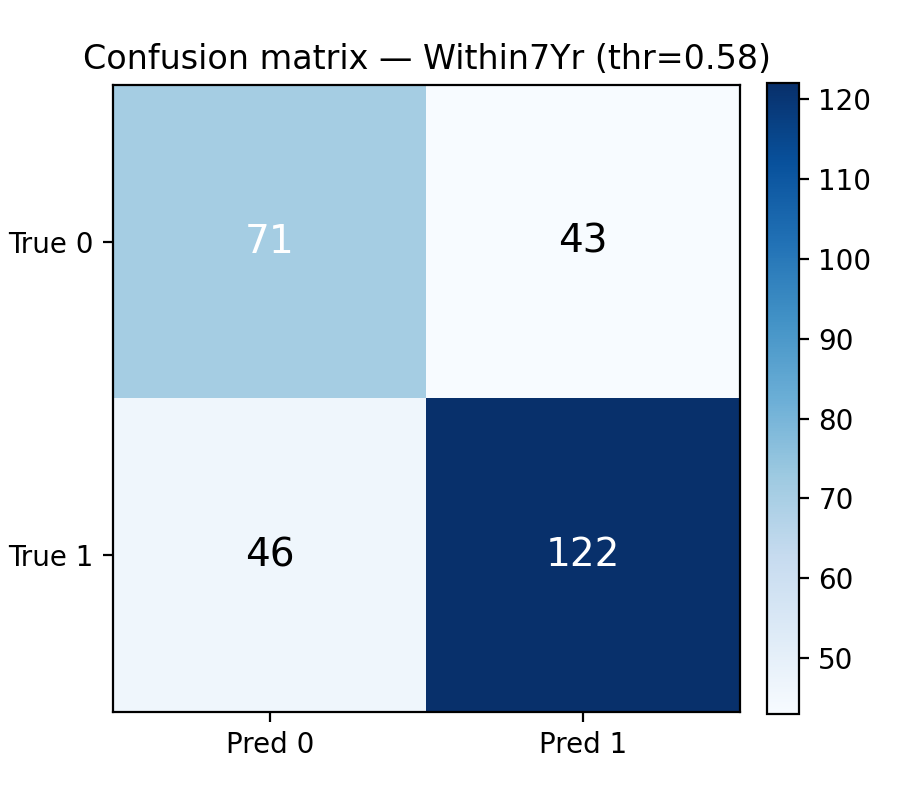
\includegraphics[width=\linewidth]{main_cmyouden_within7yr.png}
    \caption{Pooled confusion matrix at $\tau^\star=0.58$ (Youden).}
  \end{subfigure}
  \caption{Out-of-fold confusion matrices for Within7Yr. The Youden
  threshold trades off $14$ false positives for an additional $14$
  false negatives, lifting balanced accuracy from $0.646$ to $0.674$.}
  \label{fig:within7yr_cm}
\end{figure}

\subsubsection*{Reproducibly informative features (Within7Yr).}
\Cref{fig:within7yr_features} contrasts the two feature views the
pipeline produces. The stability-selection panel answers ``how often is
this feature picked across the $15$ outer training folds at any
$\ell_1$ strength?'' Several proteins (\texttt{ATP6V1F},
\texttt{179\_EGFR}, \texttt{135\_GDF-15}, \texttt{BCAN},
\texttt{IL-20RA}, \texttt{177\_FABP2}) clear the $0.95$ frequency mark
--- they are virtually always selected. The Random-Forest impurity
panel re-ranks the same shortlist by how much the trees of the final
forest \emph{actually use} each feature: \texttt{135\_GDF-15} and
\texttt{CKAP4} top this list, and the head of the importance ranking
overlaps strongly with the head of the stability ranking but is not
identical, which is what we expect when a global linear selector and a
non-linear ensemble emphasise complementary aspects of the same signal.

\begin{figure}[h]
  \centering
  \begin{subfigure}[t]{0.48\textwidth}
    \centering
    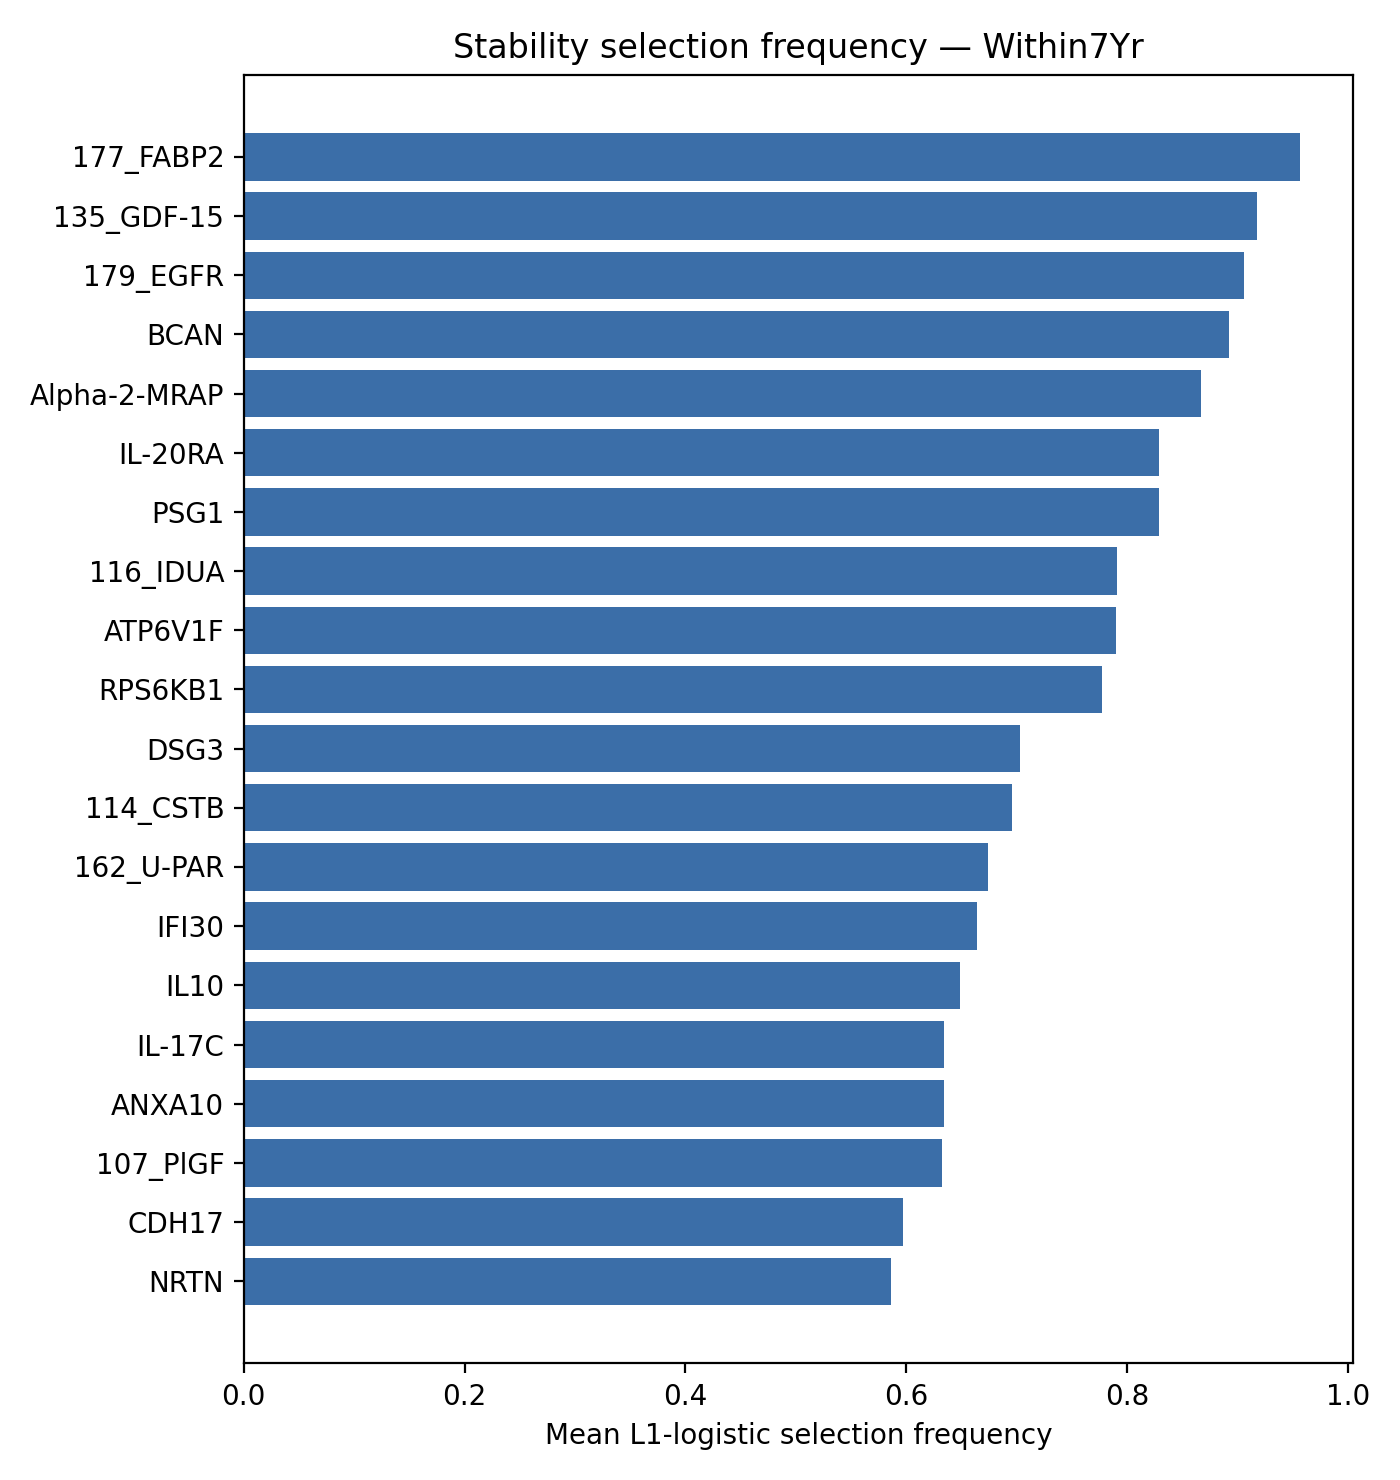
\includegraphics[width=\linewidth]{main_stability_within7yr.png}
    \caption{Stability-selection frequency.}
  \end{subfigure}
  \hfill
  \begin{subfigure}[t]{0.48\textwidth}
    \centering
    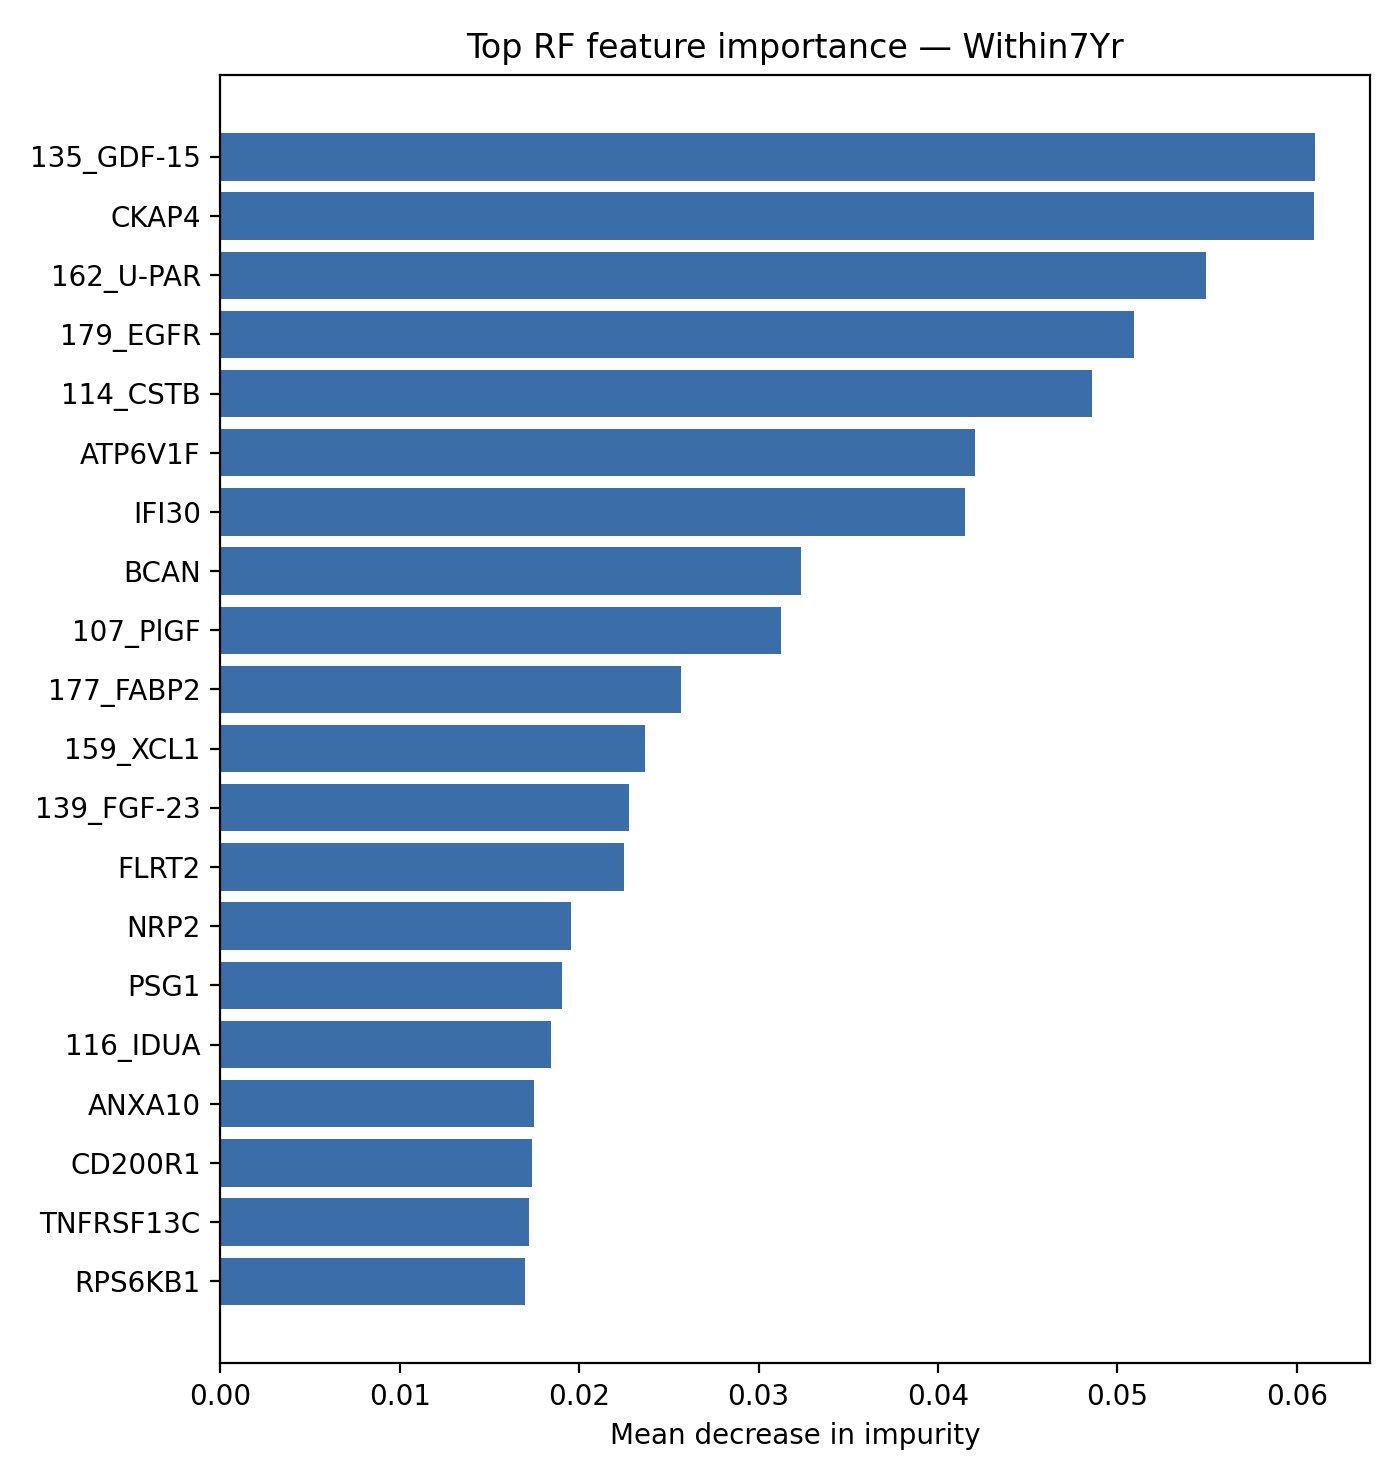
\includegraphics[width=\linewidth]{main_rfimp_within7yr.png}
    \caption{Random-Forest impurity importance.}
  \end{subfigure}
  \caption{Two complementary feature views for the Within7Yr published
  signature. (a) the L1-logistic selection frequency averaged across
  the $15$ outer training folds; (b) the impurity-based importance of
  the same features in the published forest fitted on the full data.}
  \label{fig:within7yr_features}
\end{figure}

\subsubsection*{Gradual sweep, Within7Yr.}
\Cref{fig:within7yr_gradual_all} shows ten metrics versus feature count
$k$. Discrimination metrics rise sharply over the first $\sim 5$
features, peak in the $k\!=\!19$--$26$ band, and then decay slightly as
the long tail of the ranking is added. The headline numbers are: peak
\emph{per-fold mean ROC-AUC} $=0.898 \pm 0.054$ at $k=26$, peak
\emph{average precision} $=0.936$ at $k=21$, peak \emph{balanced
accuracy} $=0.810$ at $k=19$, and minimum \emph{Brier score} $=0.138$ at
$k=14$. A rich representation of where each curve peaks across all ten
metrics simultaneously is given in
\Cref{fig:within7yr_peakmarker}.

\begin{figure}[h]
  \centering
  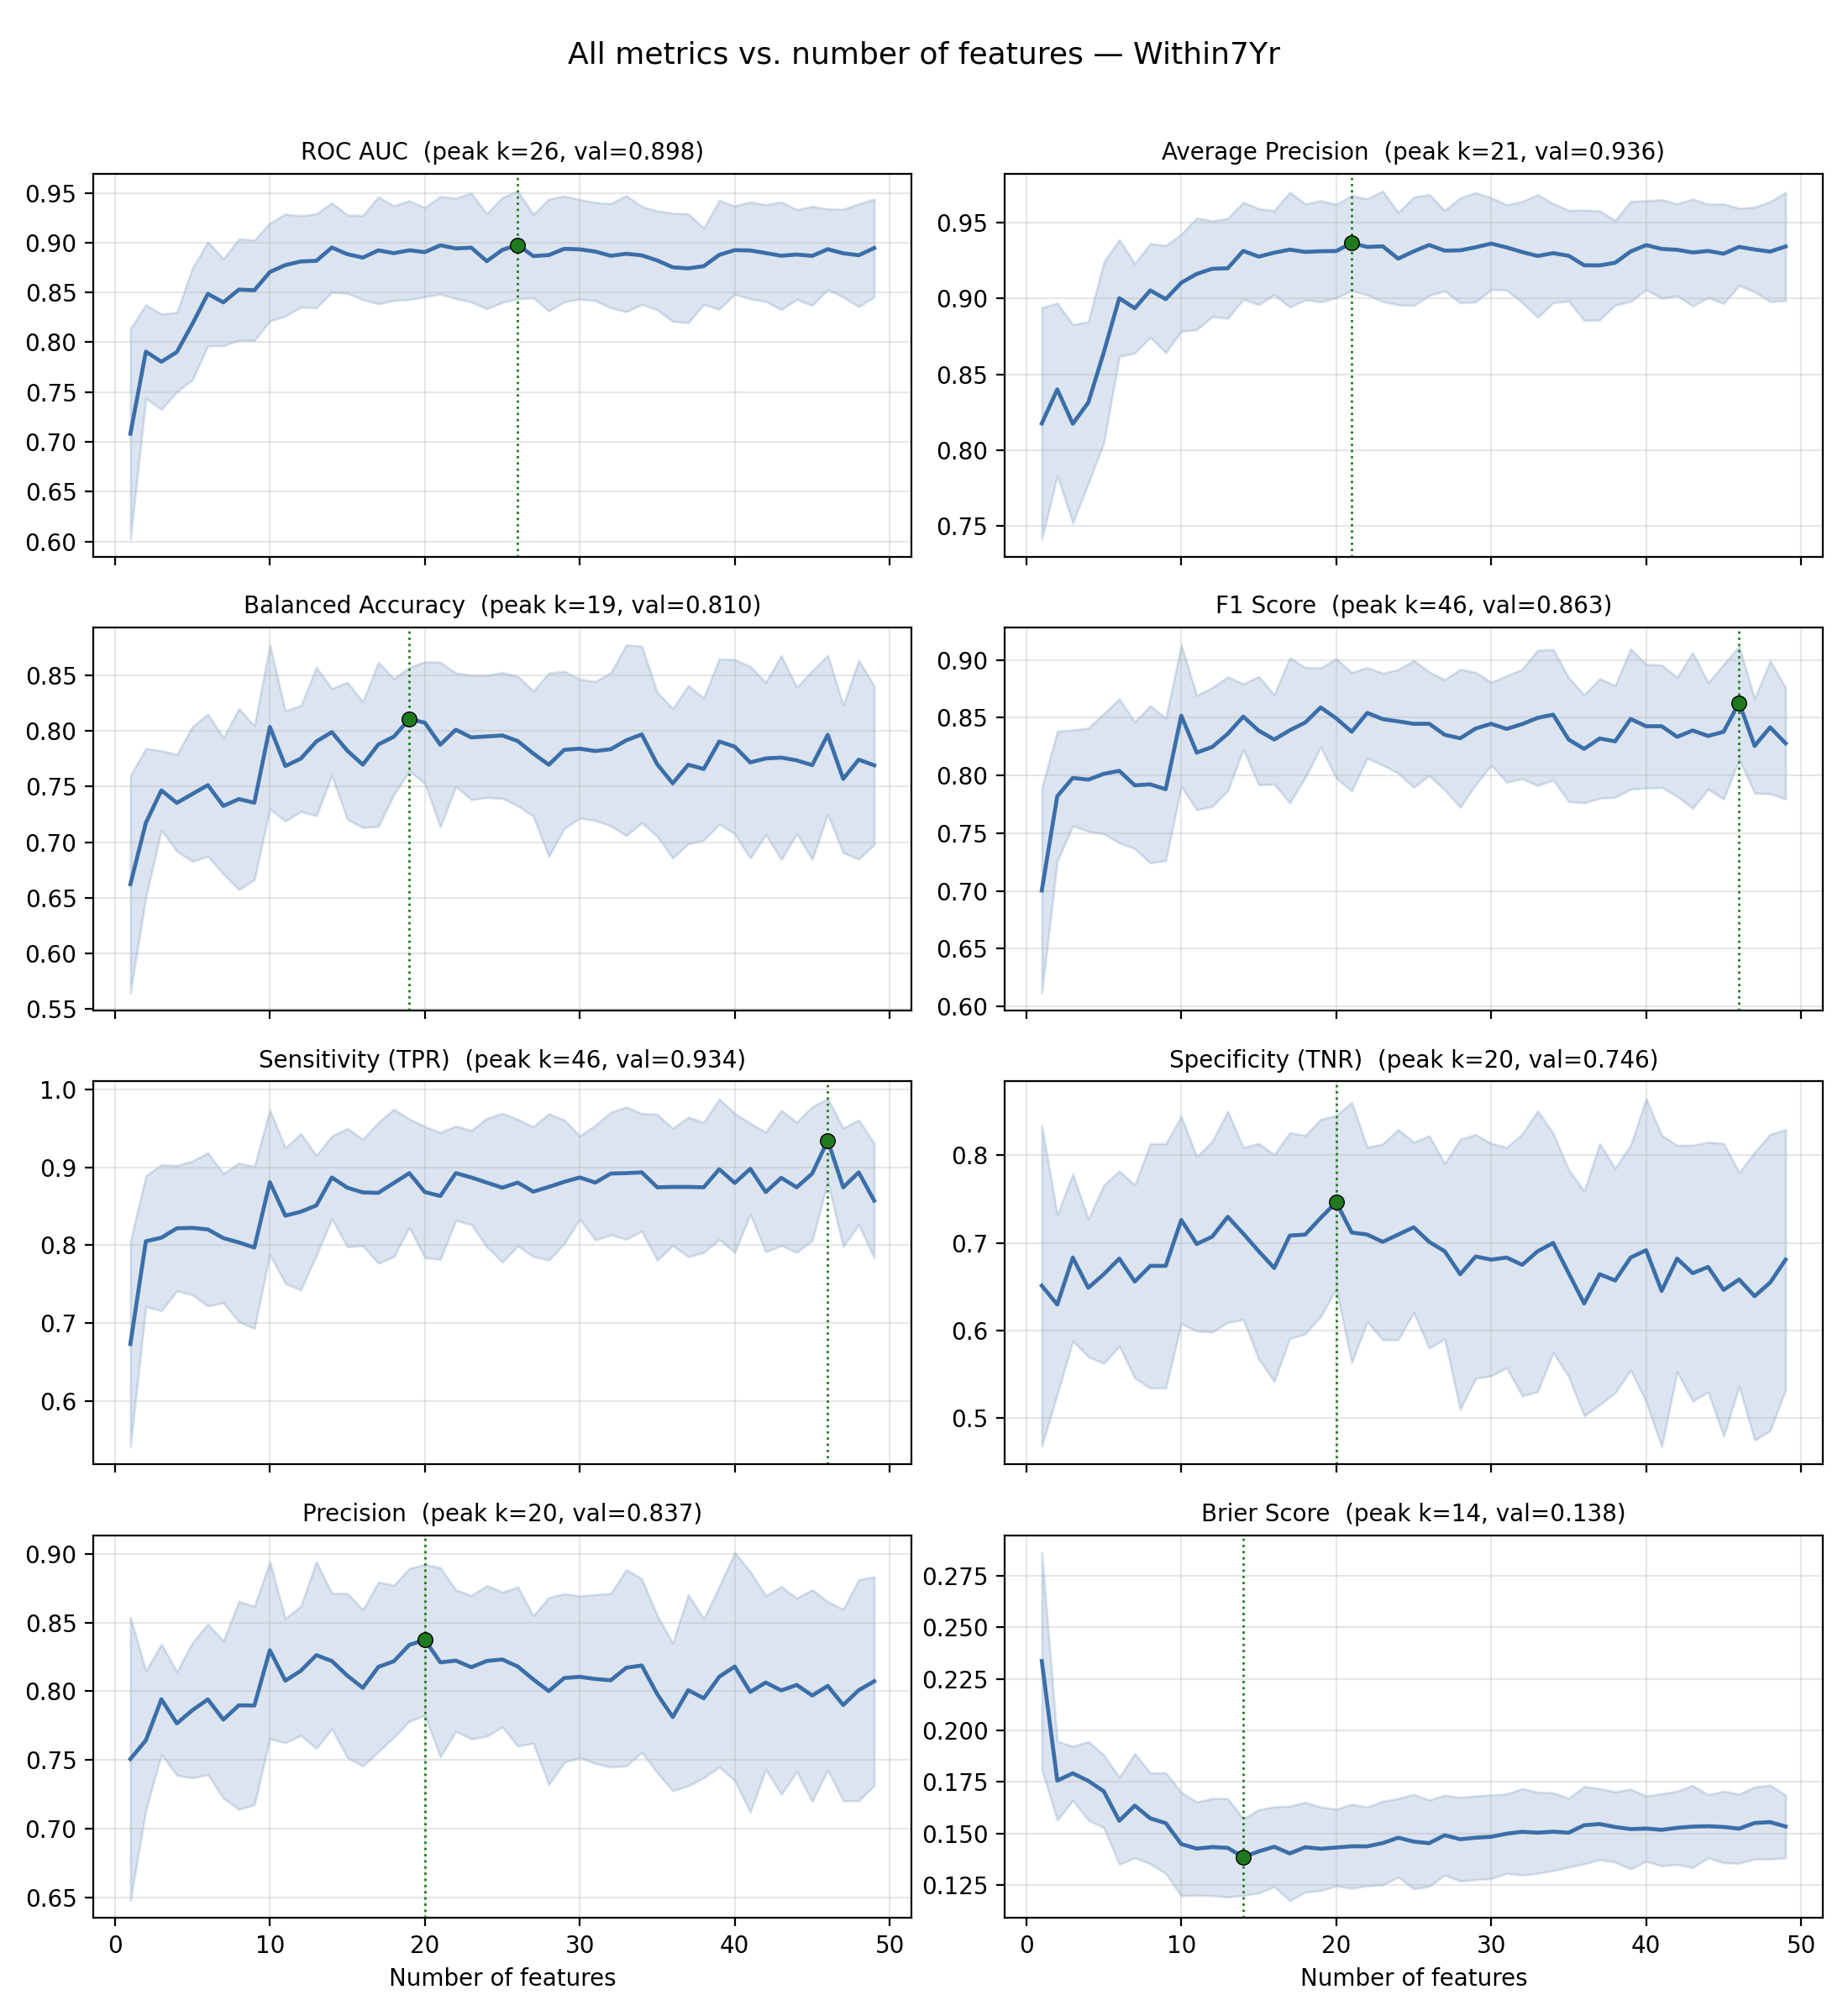
\includegraphics[width=0.95\textwidth]{gradual_allmetrics_within7yr.png}
  \caption{Within7Yr gradual sweep --- ten held-out metrics versus
  feature count $k$. Each panel: per-fold mean across the $15$ outer
  folds (line) with $\pm 1\,\mathrm{SD}$ band; vertical green guide
  marks the per-metric peak. Note the consistent ``plateau by
  $k\!\approx\!20$'' shape across discrimination metrics.}
  \label{fig:within7yr_gradual_all}
\end{figure}

\begin{figure}[h]
  \centering
  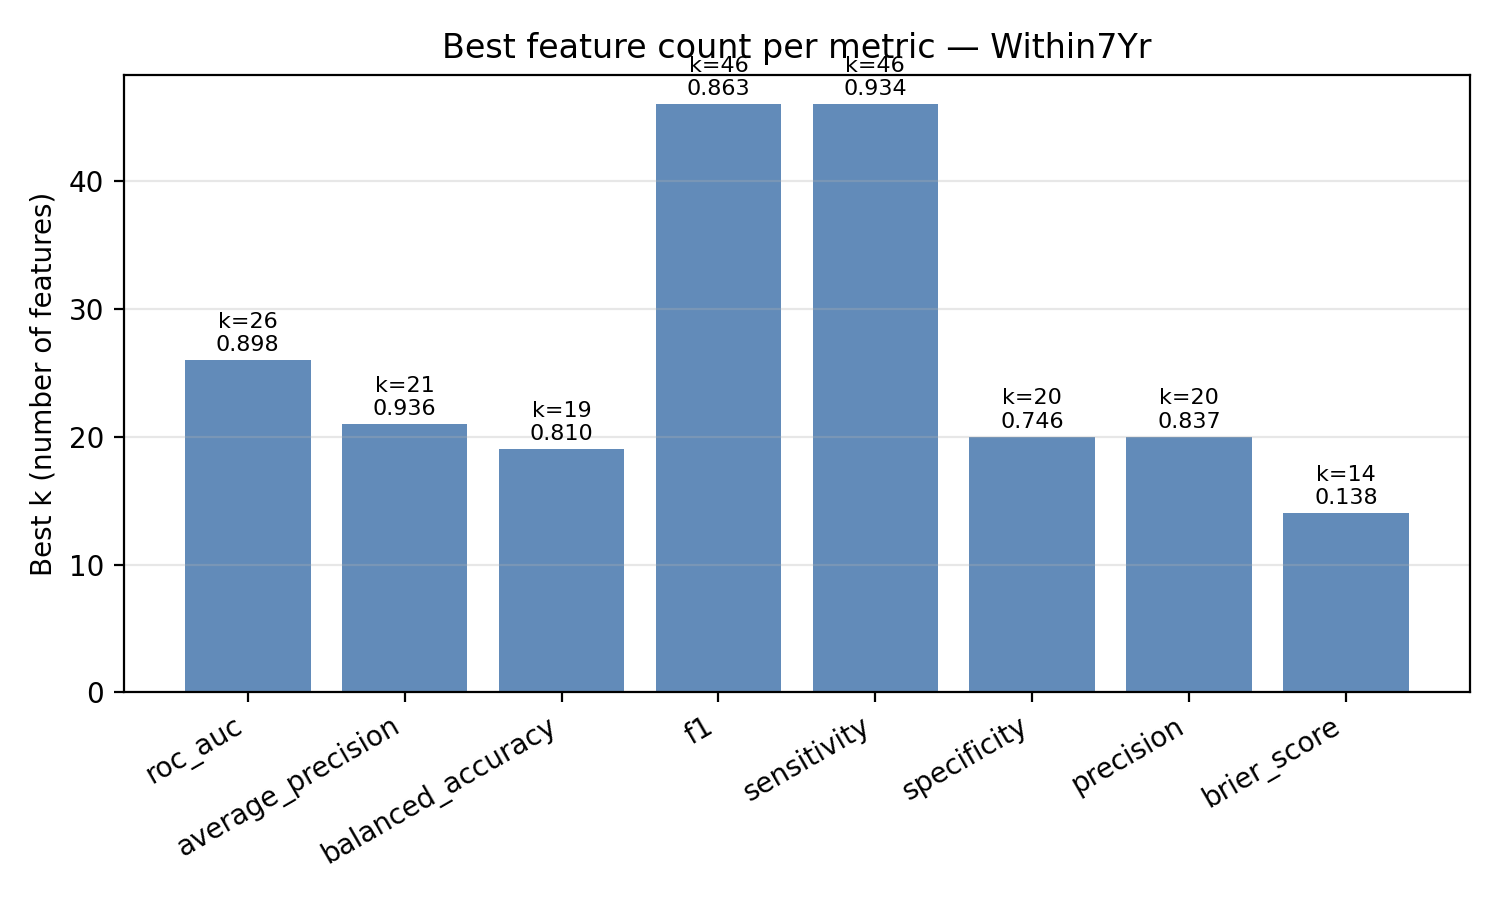
\includegraphics[width=0.95\textwidth]{gradual_peakmarker_within7yr.png}
  \caption{Within7Yr per-metric peak summary. Each row is one metric;
  the marker is placed at the $k$ that optimises that metric. Most
  discrimination peaks fall in the band $k\!=\!14$--$26$.}
  \label{fig:within7yr_peakmarker}
\end{figure}

\Cref{fig:within7yr_gradual_compare} shows pooled OOF ROC curves at
$k=1$, peak-AUC $k$, and the full published list. A single feature
($k=1$) already gives AUC$\approx 0.66$; the peak-$k$ curve reaches
AUC$=0.888$; the full list (49 features) gives AUC$=0.717$. The
``slimmer is better'' shape is clearer here than at any other horizon.

\begin{figure}[h]
  \centering
  \begin{subfigure}[t]{0.48\textwidth}
    \centering
    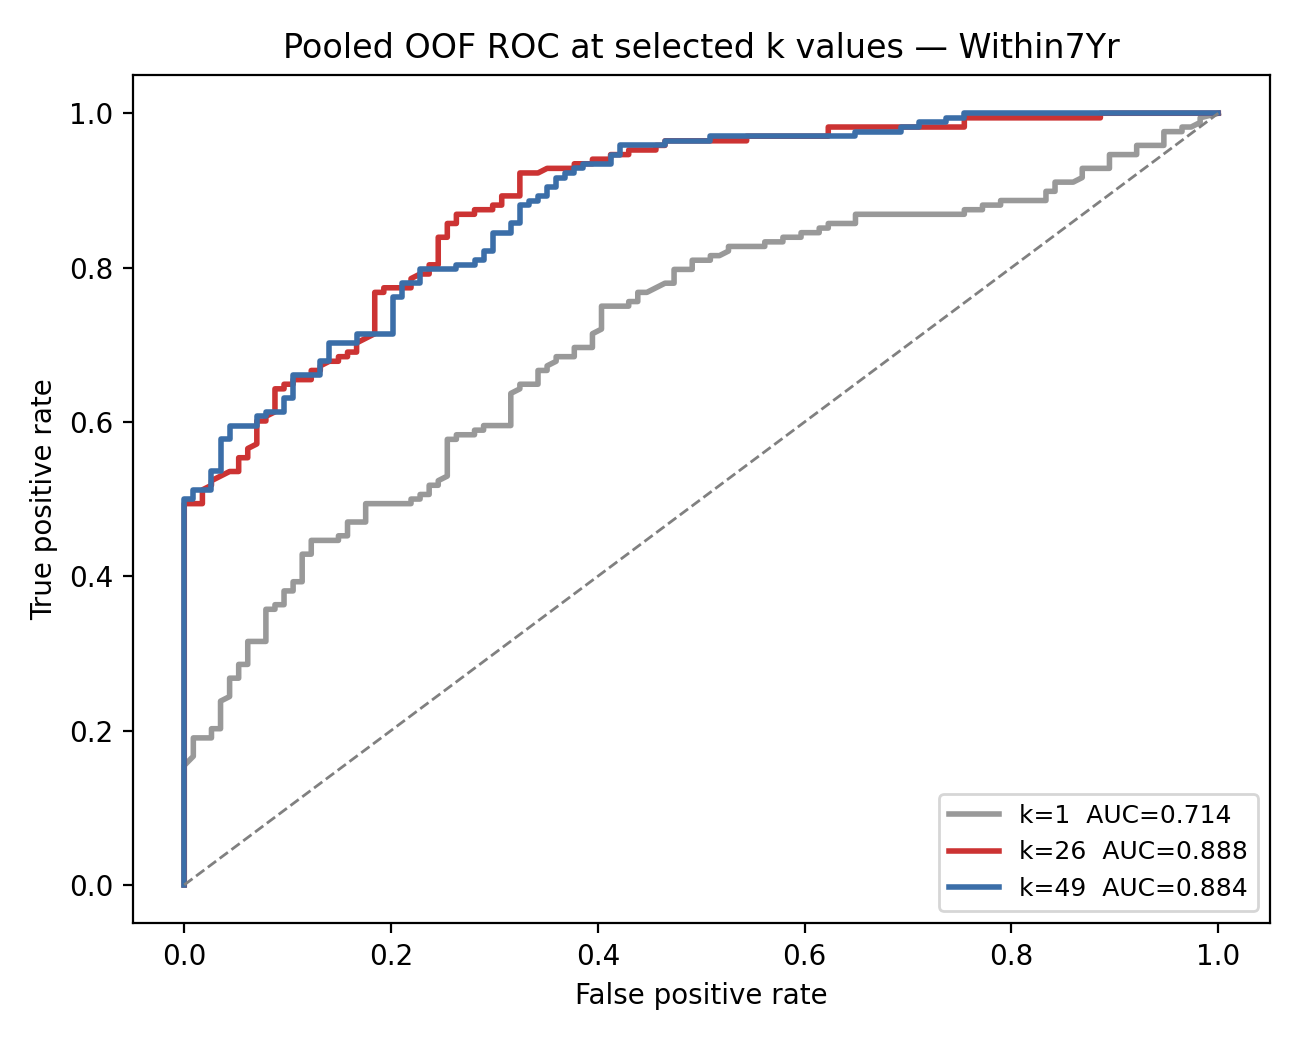
\includegraphics[width=\linewidth]{gradual_roc_within7yr.png}
    \caption{Pooled OOF ROC at three feature counts.}
  \end{subfigure}
  \hfill
  \begin{subfigure}[t]{0.48\textwidth}
    \centering
    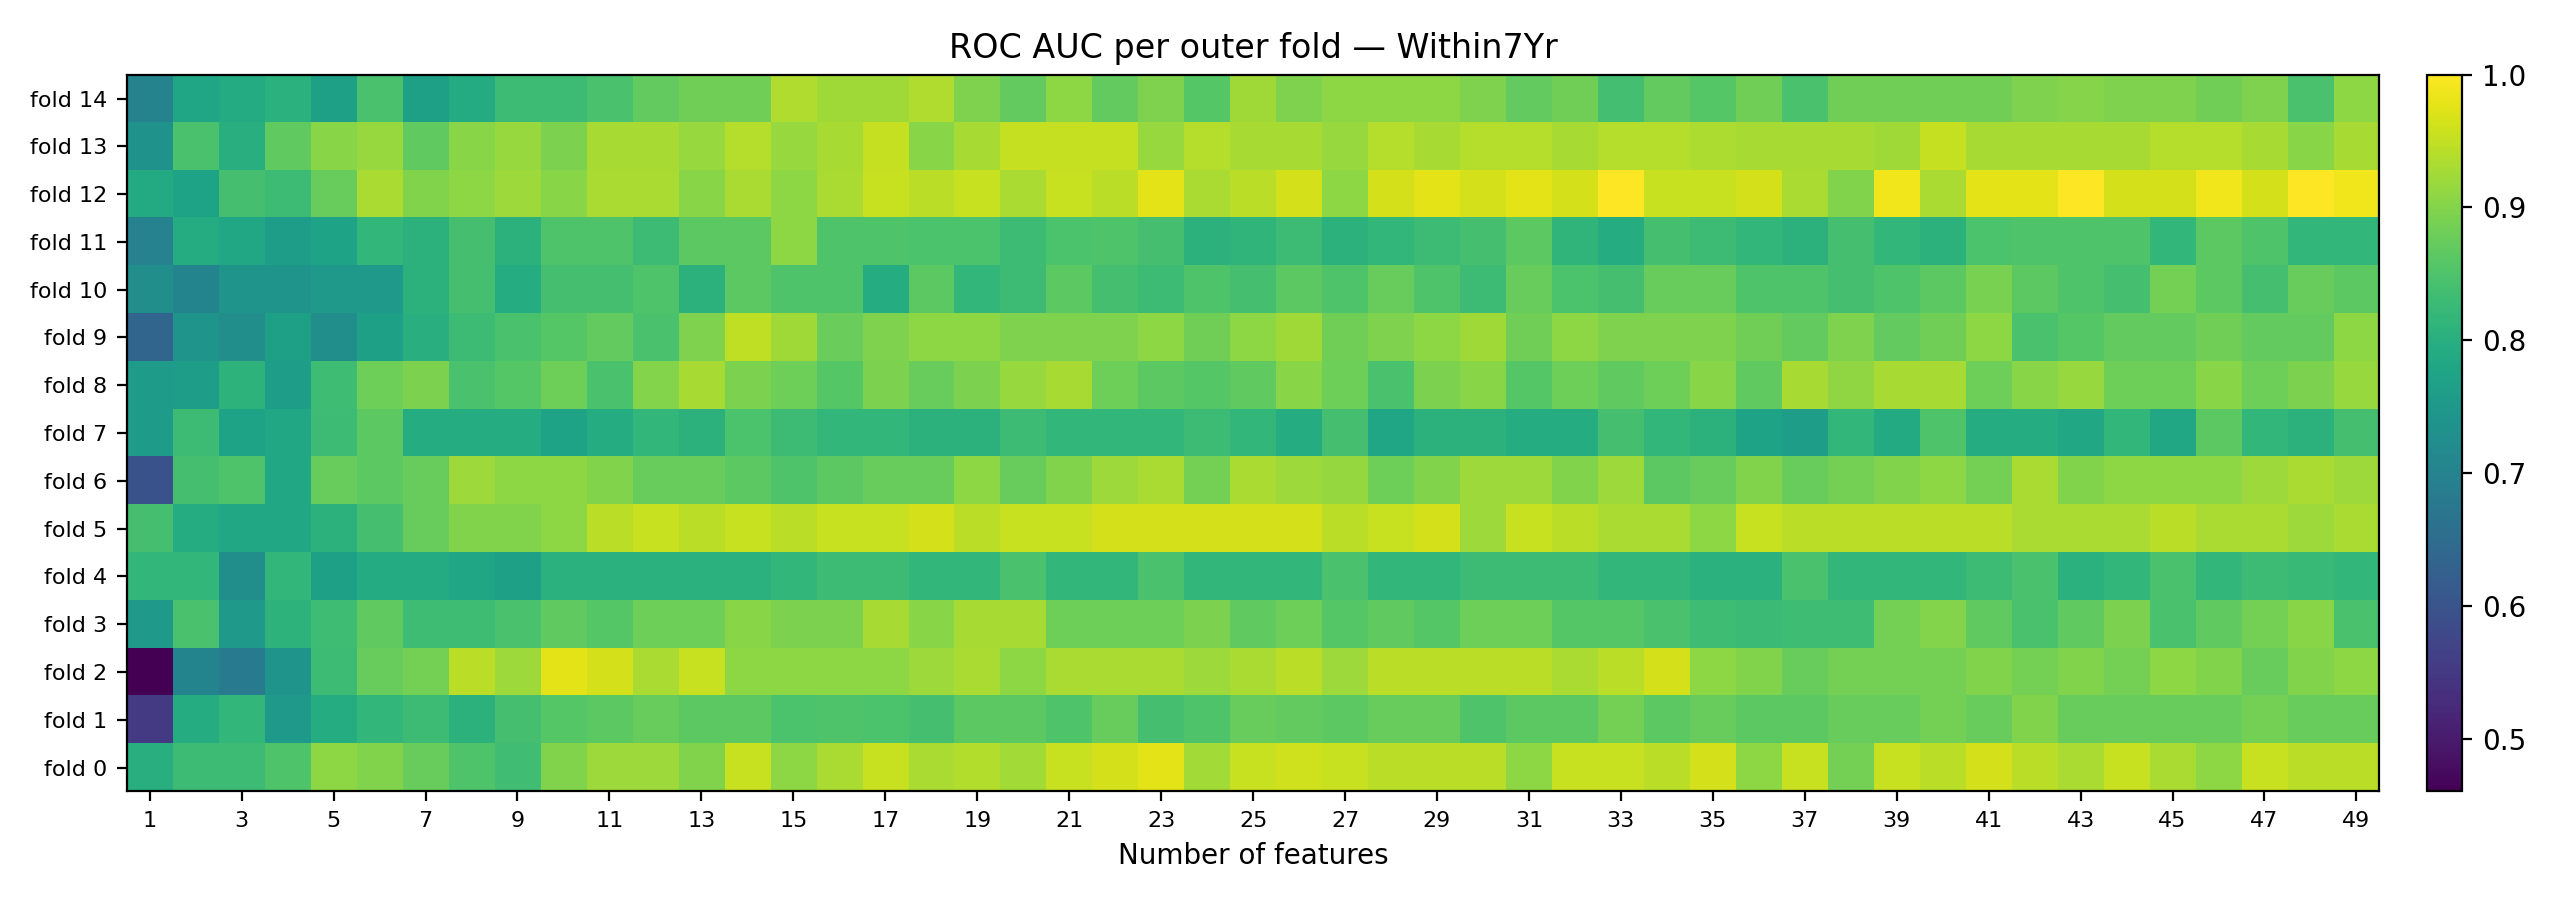
\includegraphics[width=\linewidth]{gradual_heatmap_within7yr.png}
    \caption{Per-fold ROC-AUC heatmap, $15\times 49$.}
  \end{subfigure}
  \caption{Within7Yr gradual diagnostics. The heatmap (b) shows that
  the variance is dominated by which patients fall into a given fold,
  not by the choice of $k$ within a fold; columns to the right of
  $k\!\approx\!25$ are visibly the same colour as those a few steps to
  the left, reinforcing the parsimony argument.}
  \label{fig:within7yr_gradual_compare}
\end{figure}

\subsubsection*{Auxiliary metric curves (Within7Yr).}
For full transparency we also report the standalone curves for ROC-AUC,
balanced accuracy and Brier score, with their $\pm 1$\,SD bands and
peak markers (\Cref{fig:within7yr_aux}). The Brier-score curve
(panel c) is monotonically improving up to $k\!=\!14$ and then
plateaus, mirroring the AUC story but on the calibration side.

\begin{figure}[h]
  \centering
  \begin{subfigure}[t]{0.32\textwidth}
    \centering
    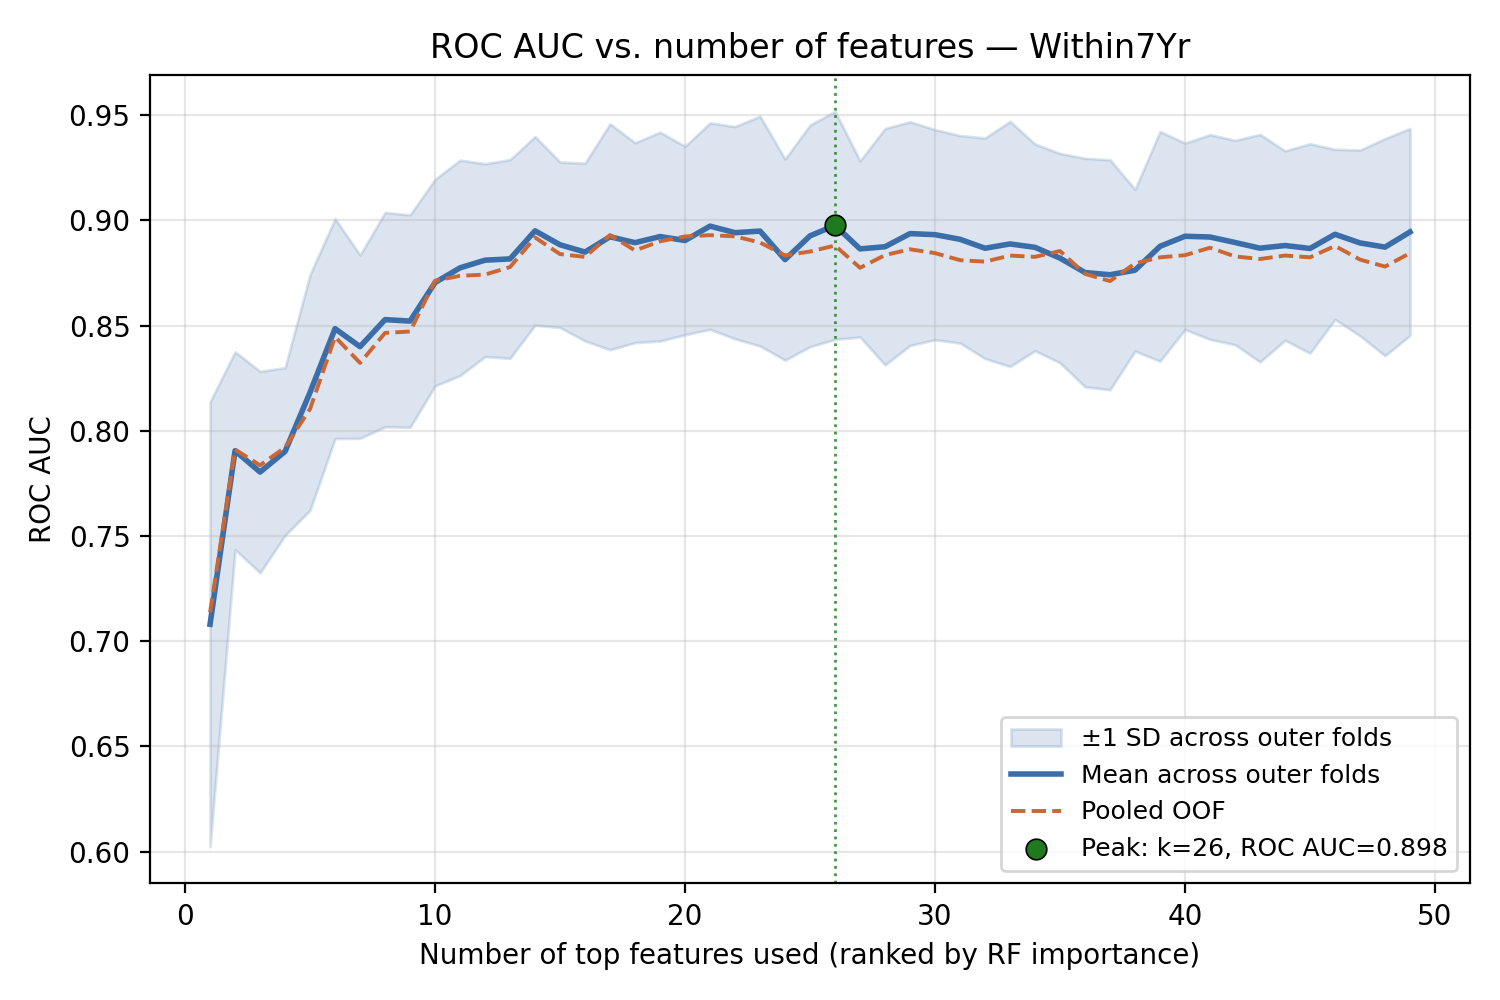
\includegraphics[width=\linewidth]{gradual_auc_within7yr.png}
    \caption{ROC-AUC vs.\ $k$.}
  \end{subfigure}
  \hfill
  \begin{subfigure}[t]{0.32\textwidth}
    \centering
    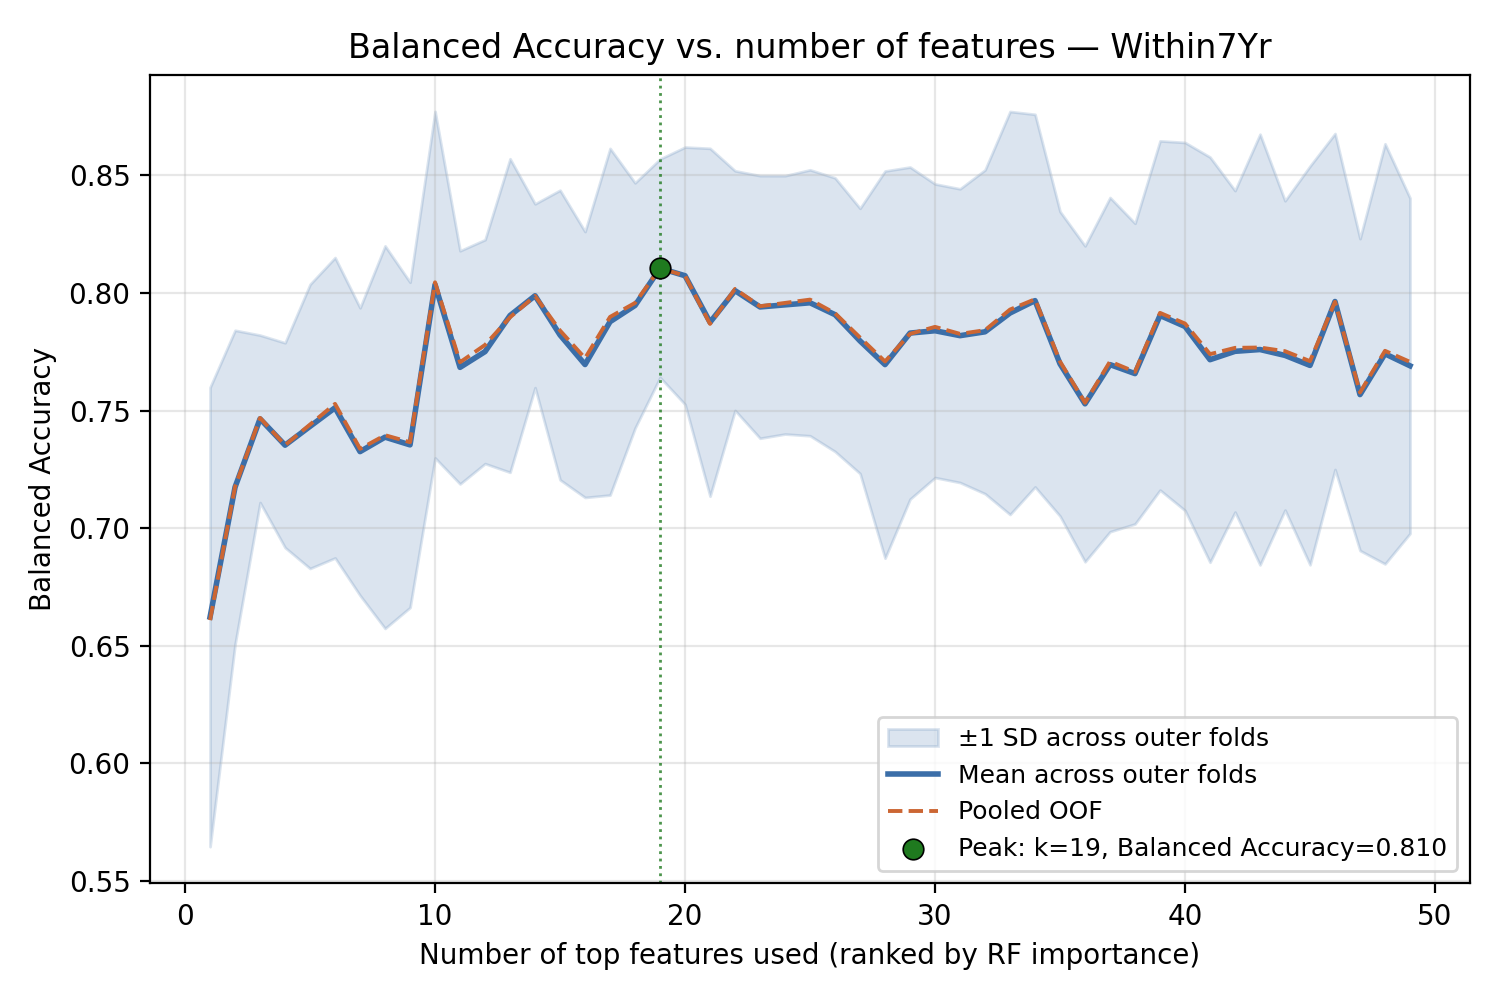
\includegraphics[width=\linewidth]{gradual_balacc_within7yr.png}
    \caption{Balanced accuracy.}
  \end{subfigure}
  \hfill
  \begin{subfigure}[t]{0.32\textwidth}
    \centering
    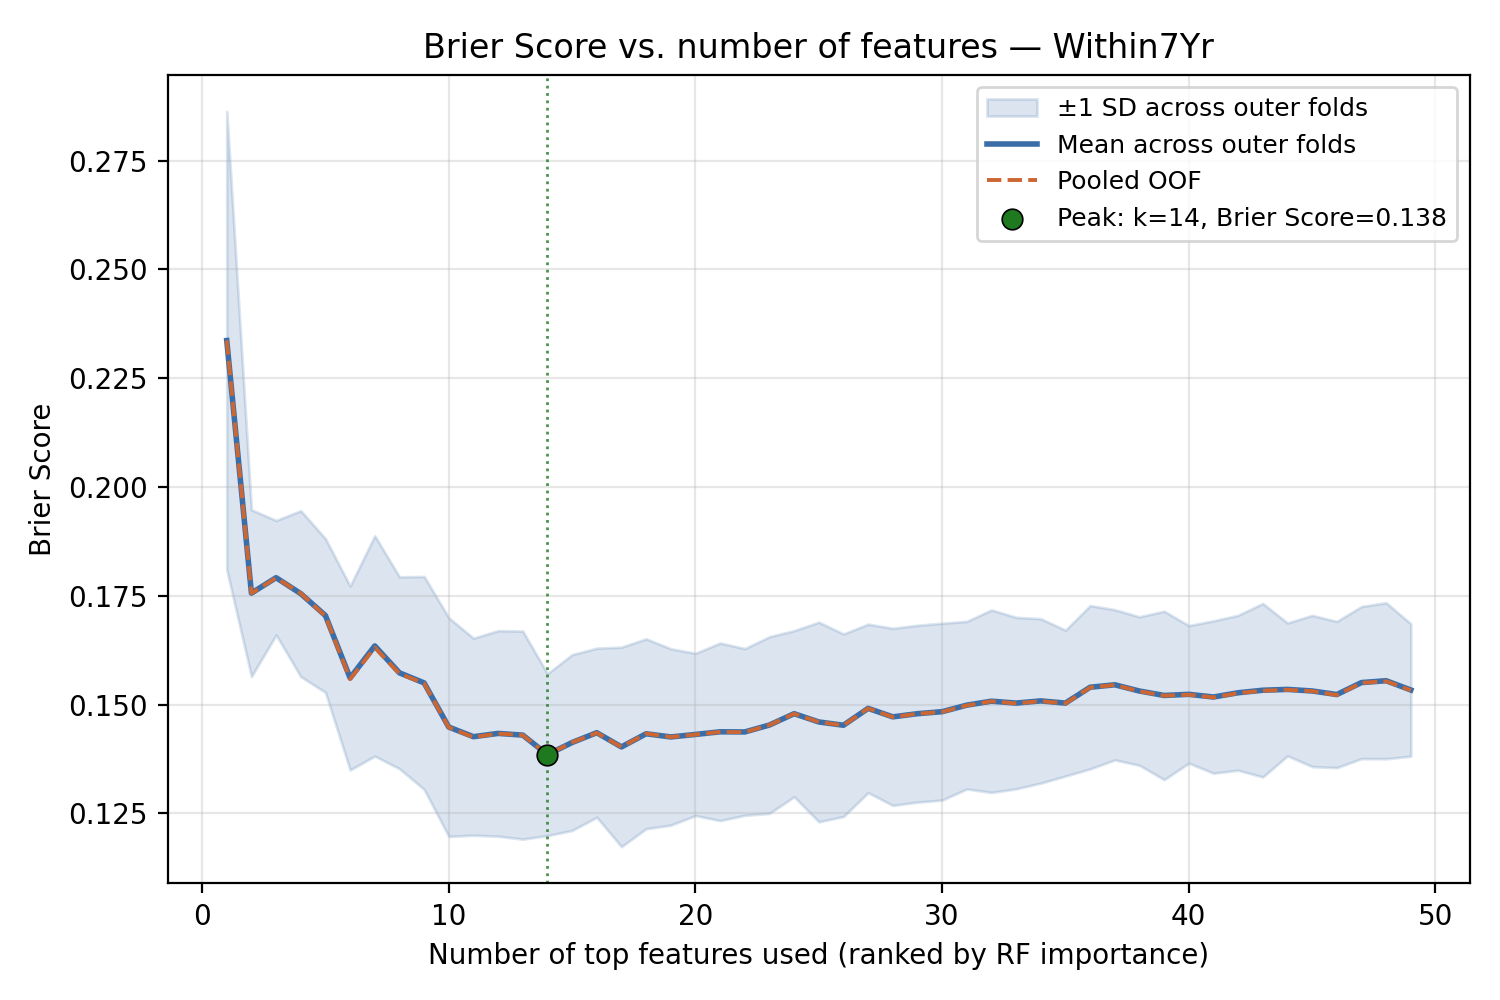
\includegraphics[width=\linewidth]{gradual_brier_within7yr.png}
    \caption{Brier (lower is better).}
  \end{subfigure}
  \caption{Within7Yr per-metric curves. Each panel: per-fold mean
  (blue) with $\pm 1$\,SD band; pooled OOF curve (orange dashed); peak
  marker in green.}
  \label{fig:within7yr_aux}
\end{figure}

\begin{figure}[h]
  \centering
  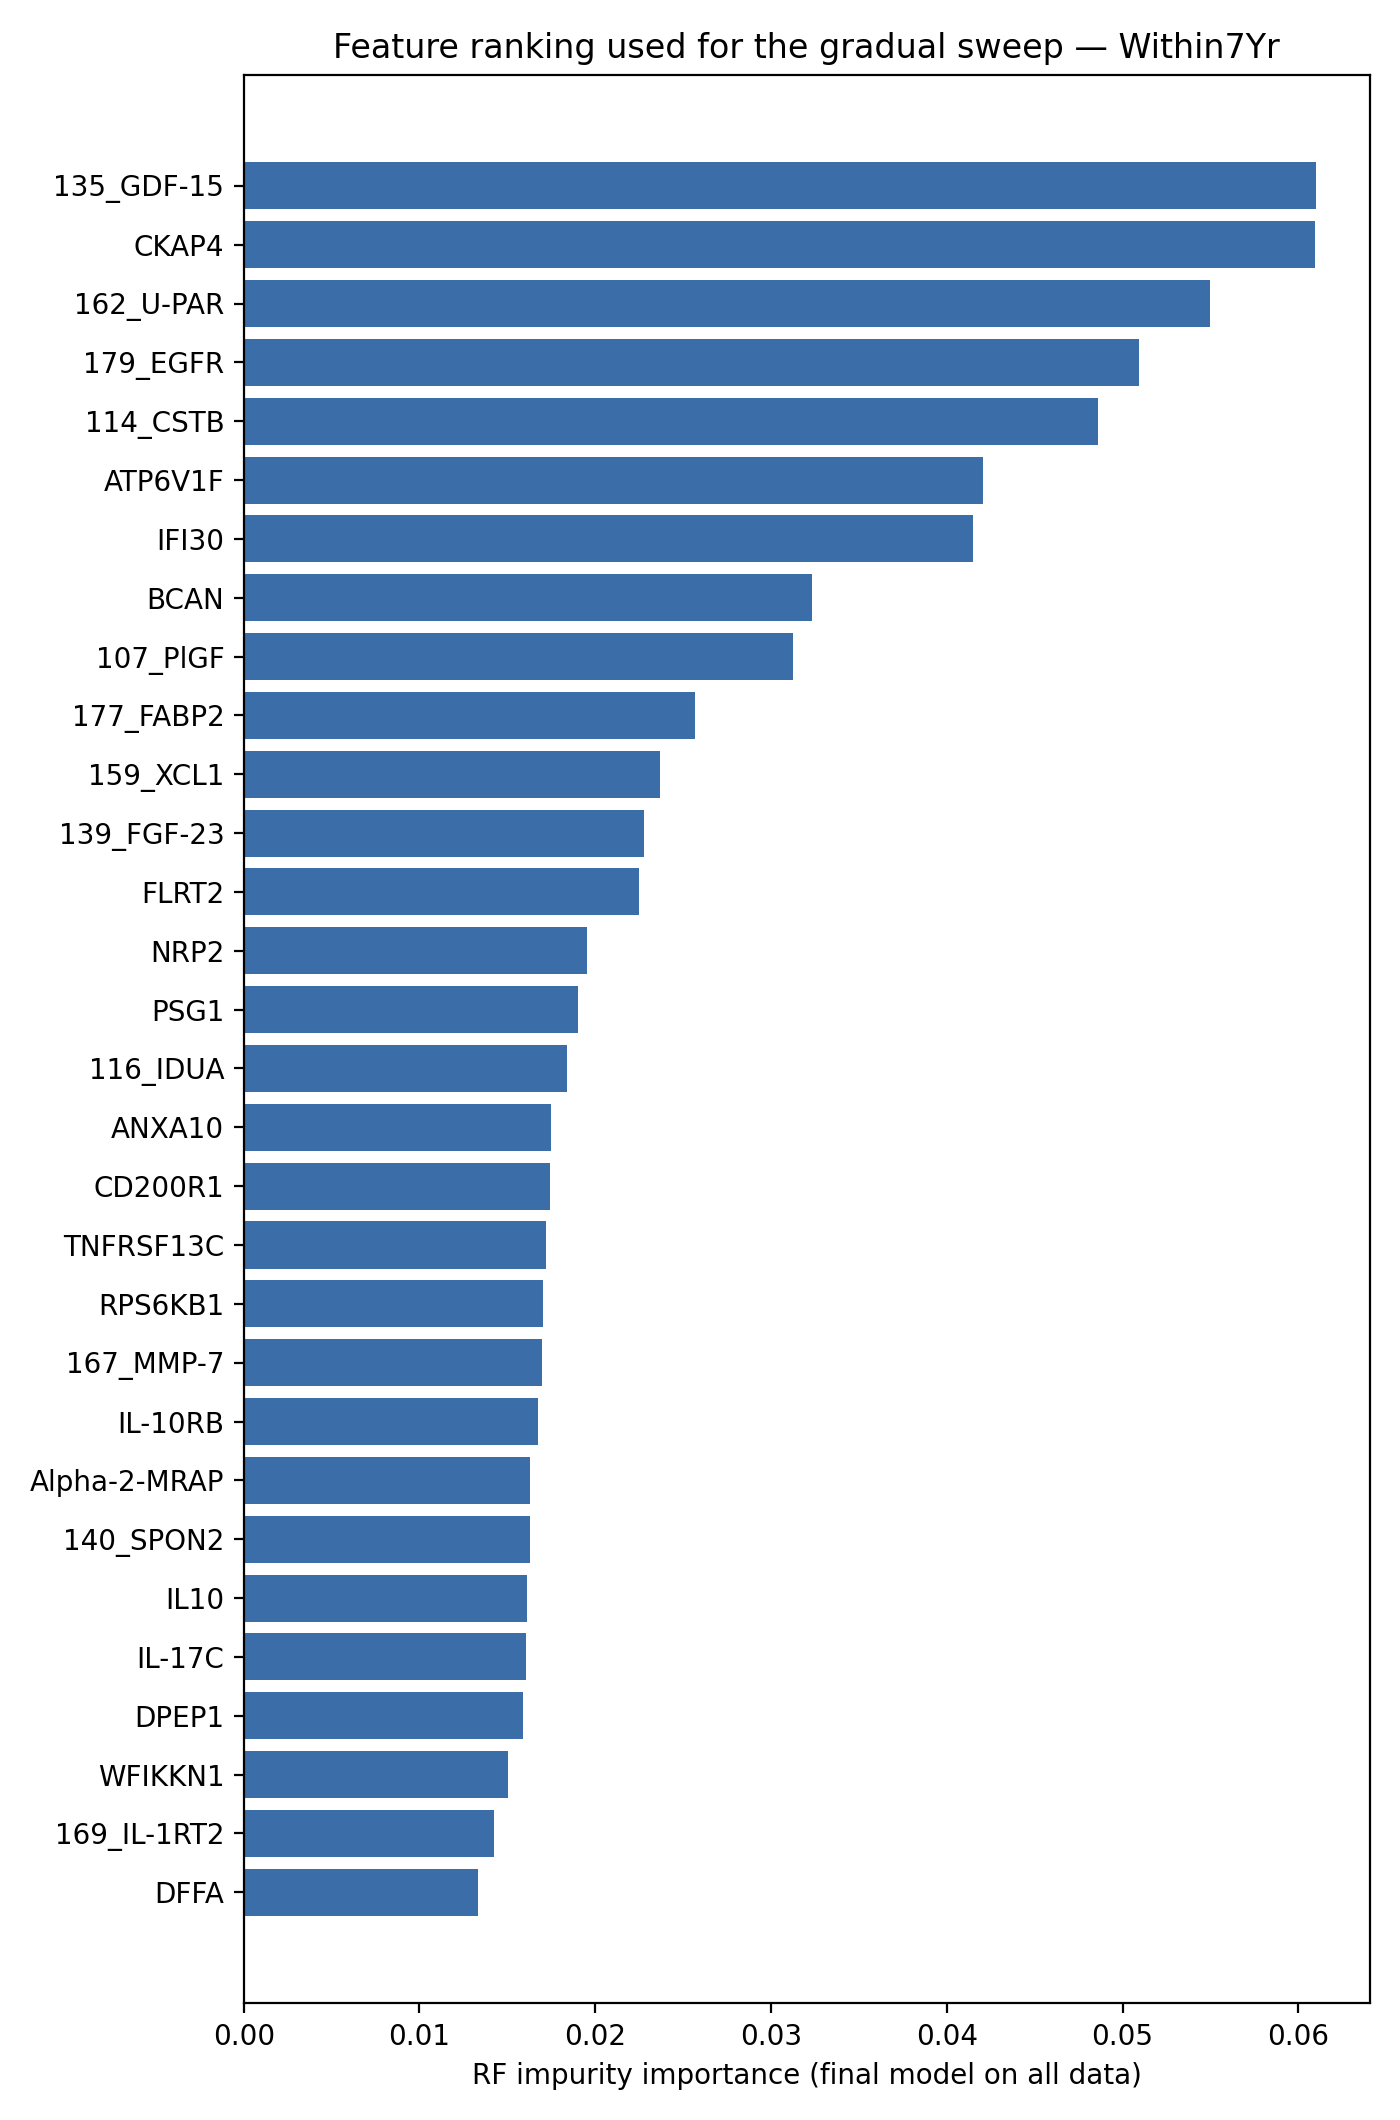
\includegraphics[width=0.85\textwidth]{gradual_features_within7yr.png}
  \caption{Within7Yr feature ranking used by the gradual sweep
  (top entries by RF impurity importance from the published forest).
  This is the order in which features are added when $k$ is increased.}
  \label{fig:within7yr_ranking}
\end{figure}

\subsection{Reproducibly informative features (stability selection)}
\Cref{fig:stability} shows the top-20 features by mean stability-selection
frequency across the $15$ outer training folds for the Within3Yr
horizon. Several features (e.g.\ \texttt{LAG3}, \texttt{186\_MMP-3},
\texttt{179\_EGFR}, \texttt{CD83}) are selected in \emph{every} outer
fold, while a long tail of features cross the $0.60$ threshold
intermittently. This per-feature reproducibility is precisely what
stability selection is designed to expose, and it provides a defensible
shortlist for downstream biological interpretation.

\begin{figure}[h]
  \centering
  \begin{subfigure}[t]{0.48\textwidth}
    \centering
    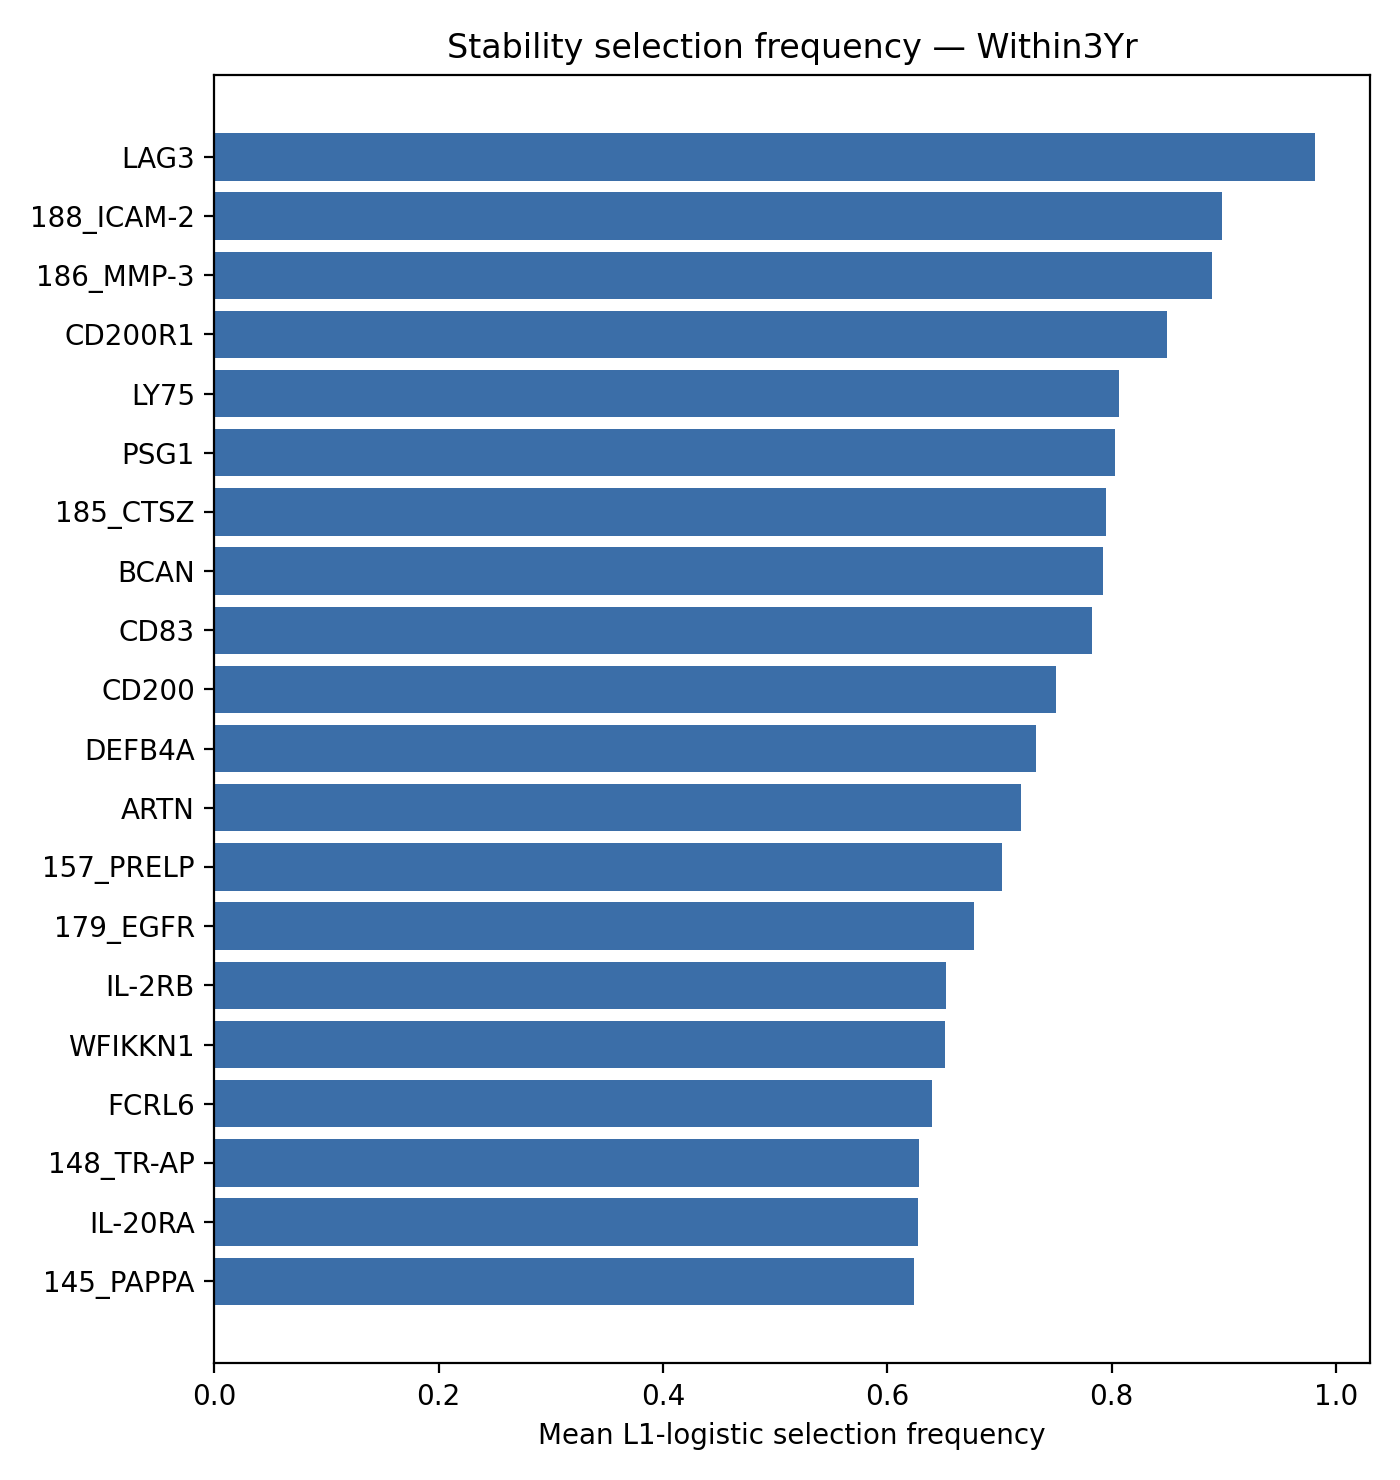
\includegraphics[width=\linewidth]{main_stability_within3yr.png}
    \caption{Stability selection frequency.}
  \end{subfigure}
  \hfill
  \begin{subfigure}[t]{0.48\textwidth}
    \centering
    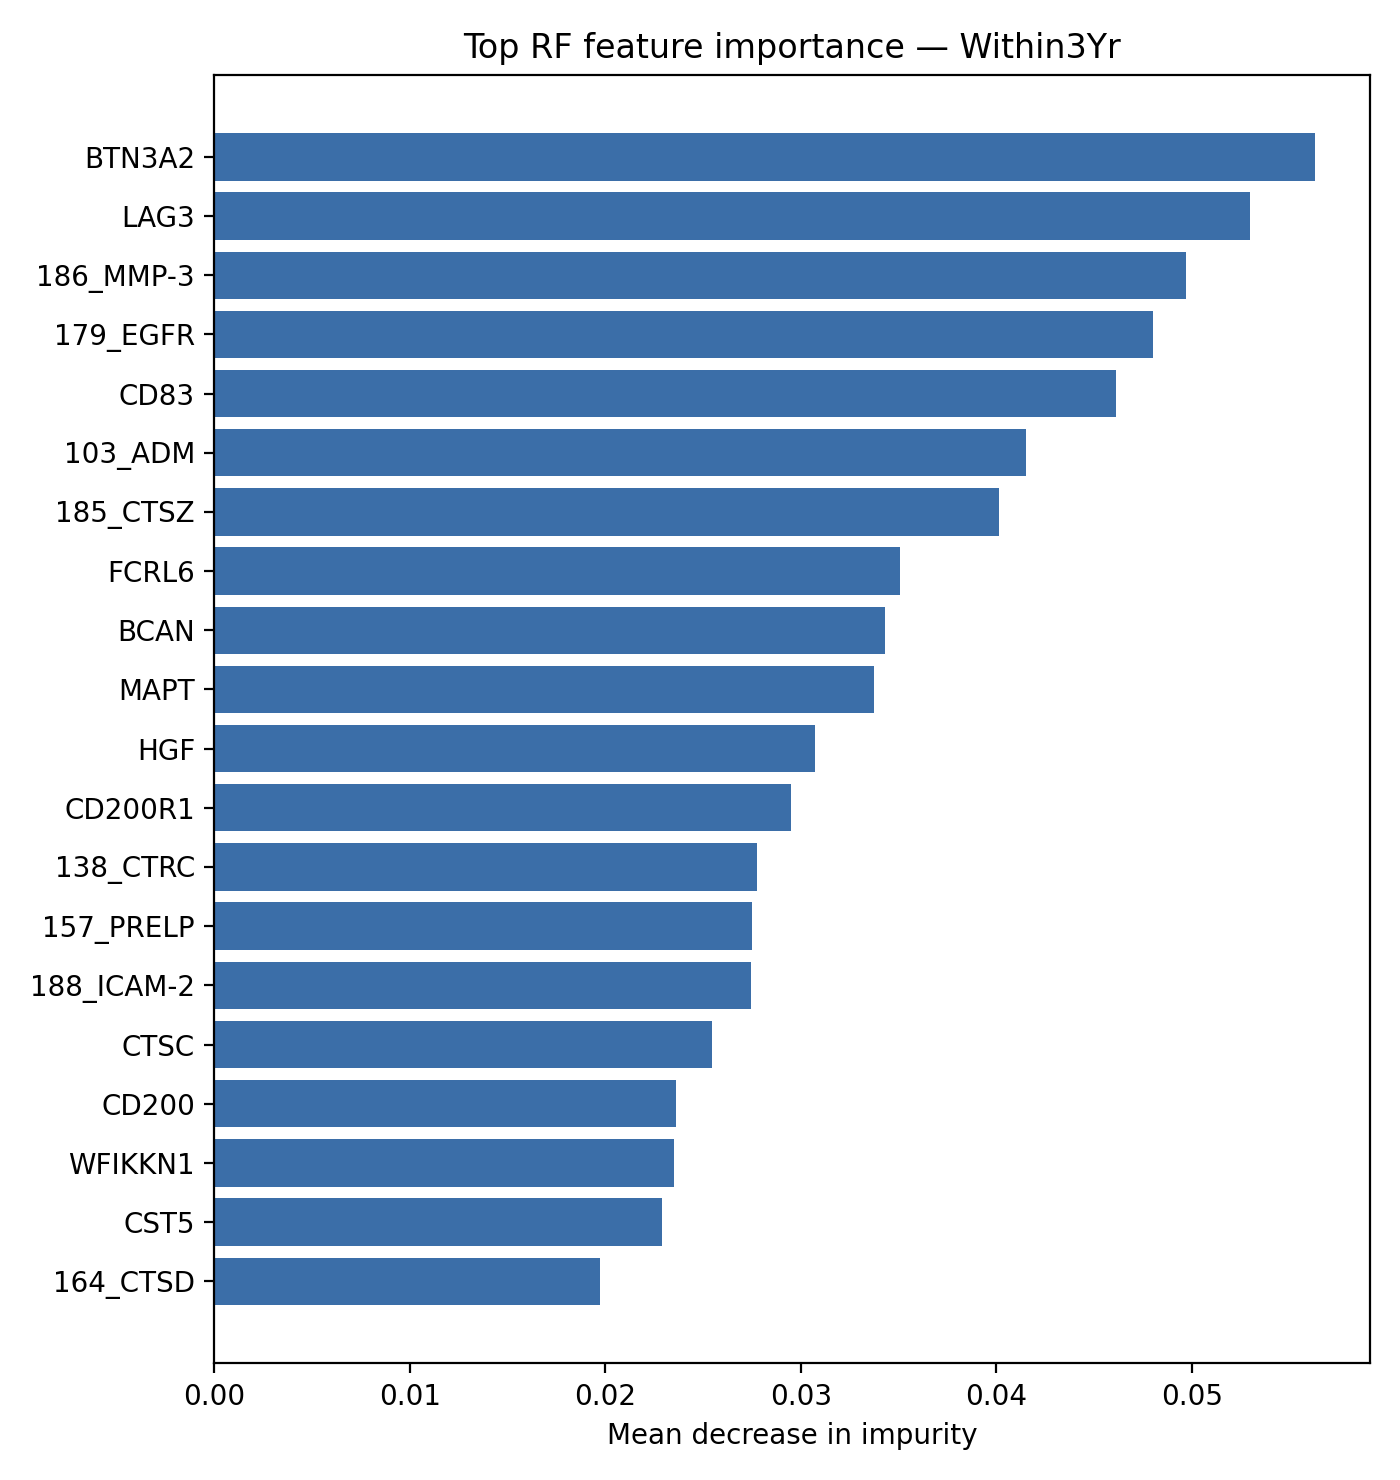
\includegraphics[width=\linewidth]{main_rfimp_within3yr.png}
    \caption{Random-Forest impurity importance.}
  \end{subfigure}
  \caption{Two complementary views of feature importance for the Within3Yr
  horizon. Stability selection answers the question ``which features are
  reproducibly chosen?'' across resamples; impurity importance answers
  ``which features actually drive the trees of the final forest?''}
  \label{fig:stability}
\end{figure}

\subsection{Gradual-training analysis: how many features do we really need?}
\label{sec:gradual_within3yr_subsec}

The gradual sweep (\Cref{sec:gradual}) walks down the published
RF-importance ranking and re-evaluates the model at every truncation.
\Cref{fig:gradual_within3yr} aggregates eight metrics versus feature
count for the Within3Yr horizon. The curves show the diagnostically
important pattern: a steep early gain that plateaus, with peak per-fold
mean ROC-AUC at $k=34$ (versus $|\mathcal{F}|=48$ for the published
list), and per-fold mean Balanced Accuracy peaking far earlier at $k=23$.
This justifies a parsimony argument: the long tail of the published list
adds little to held-out performance, despite the long tail of the
original ranking.

\begin{figure}[h]
  \centering
  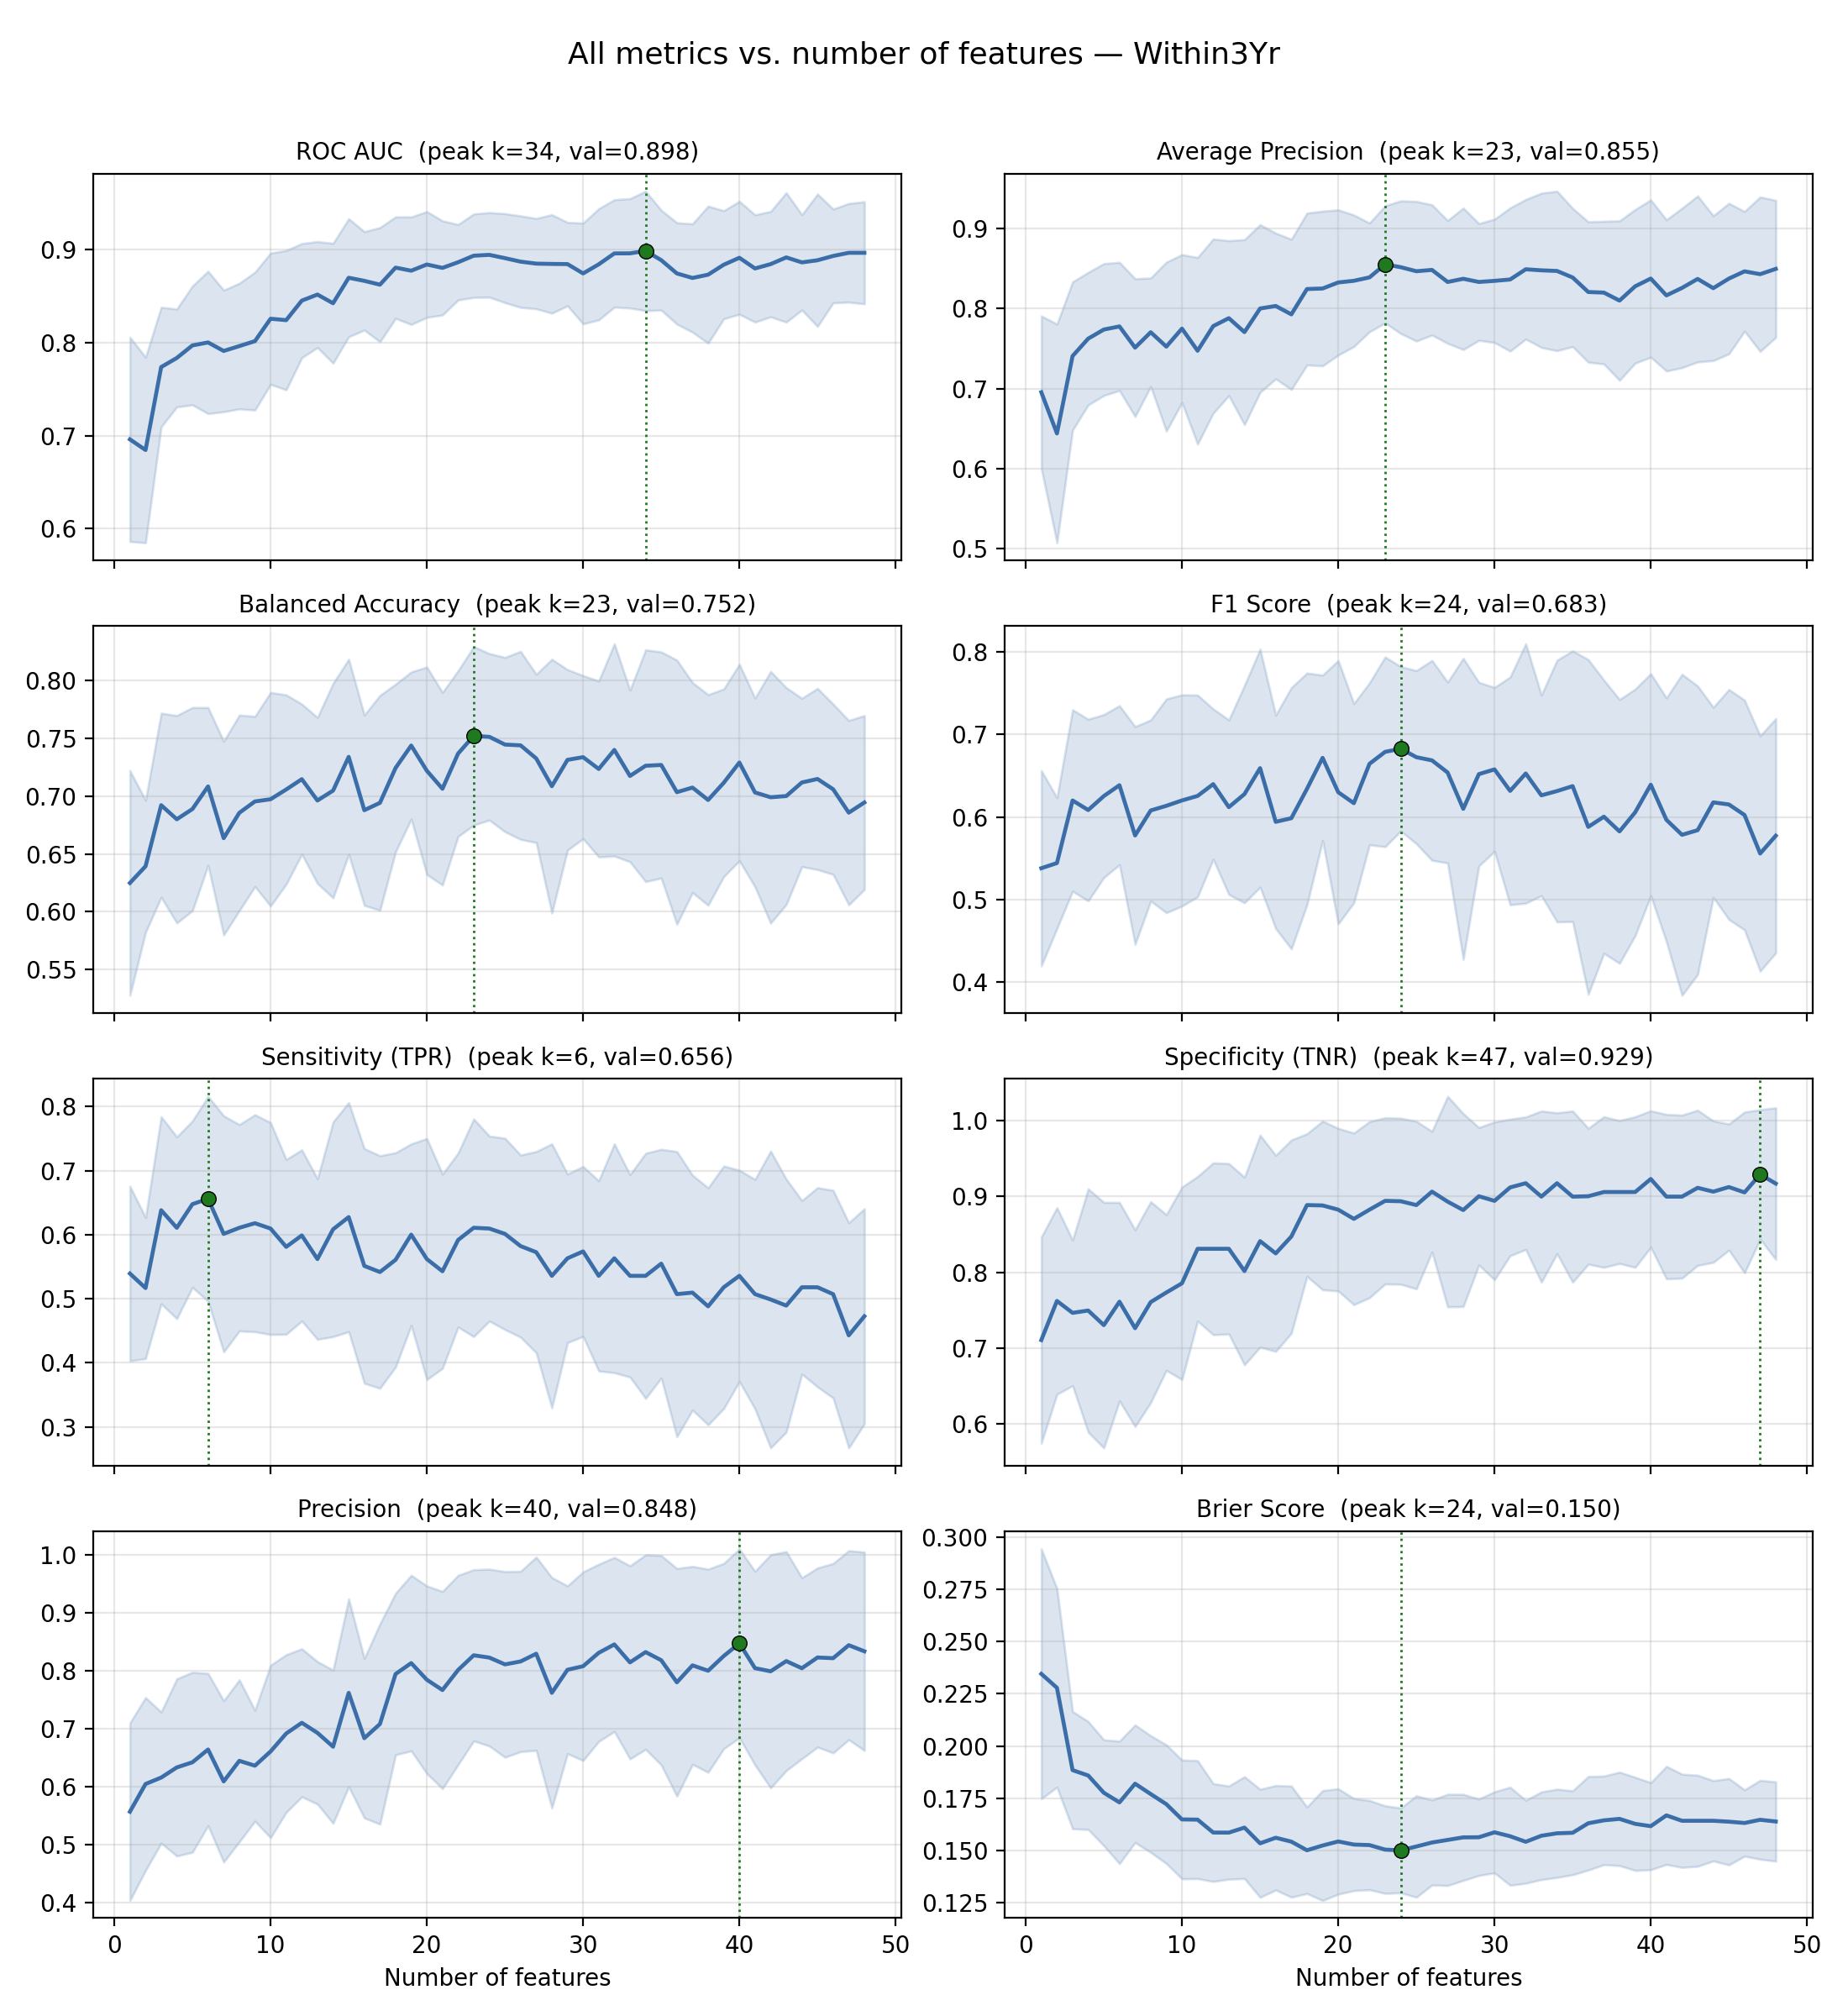
\includegraphics[width=0.95\textwidth]{gradual_allmetrics_within3yr.png}
  \caption{Gradual-training: eight held-out metrics versus number of
  features ($k$) for Within3Yr. Each panel shows the mean across the
  $15$ outer folds (line) with $\pm 1$ SD band (shaded). Green dots and
  vertical guides mark the per-metric peak. ROC-AUC peaks at $k=34$;
  Balanced Accuracy and $F_1$ peak earlier, around $k=23$--$24$.}
  \label{fig:gradual_within3yr}
\end{figure}

A finer-grained per-metric view is shown in \Cref{fig:gradual_auc_within3yr}.
The pooled OOF curve (orange dashed) and the across-fold mean (blue) are
in close agreement, while the $\pm 1\,\mathrm{SD}$ band tightens
substantially as $k$ grows beyond about $10$, which is consistent with
small-feature-set noise dominating at low $k$ and the trees stabilising
once the most informative variables have been included.

\begin{figure}[h]
  \centering
  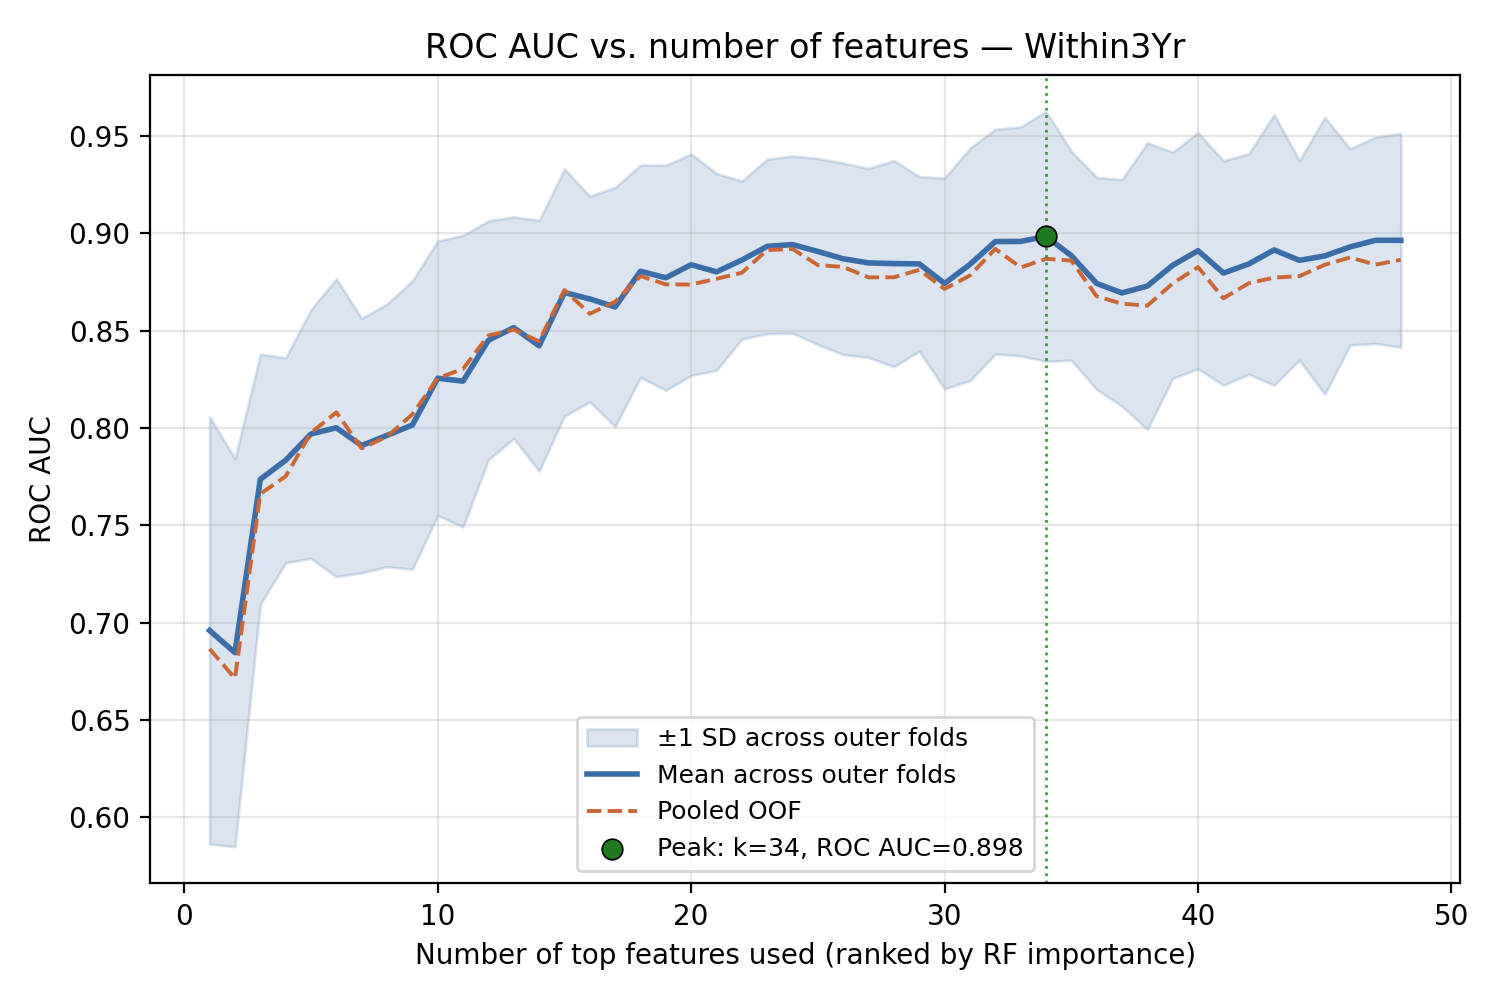
\includegraphics[width=0.62\textwidth]{gradual_auc_within3yr.png}
  \caption{Within3Yr ROC-AUC vs.\ feature count. Mean across folds (blue)
  with $\pm 1$ SD band; pooled OOF curve (orange dashed); peak at $k=34$
  marked in green.}
  \label{fig:gradual_auc_within3yr}
\end{figure}

\Cref{fig:gradual_roc_within3yr} compares pooled OOF ROC curves at three
characteristic feature counts --- $k=1$ (a single proteomic biomarker),
$k=k^\star_{\mathrm{AUC}}=34$ (peak across the sweep), and
$k=|\mathcal{F}|=48$ (the published list). The $k=1$ curve already
encodes a non-trivial signal (AUC$\approx 0.66$), the peak-$k$ curve
reaches AUC$\approx 0.89$, and adding the remaining $14$ features beyond
the peak slightly worsens the curve --- evidence that the long tail is
predominantly noise on this cohort size.

\begin{figure}[h]
  \centering
  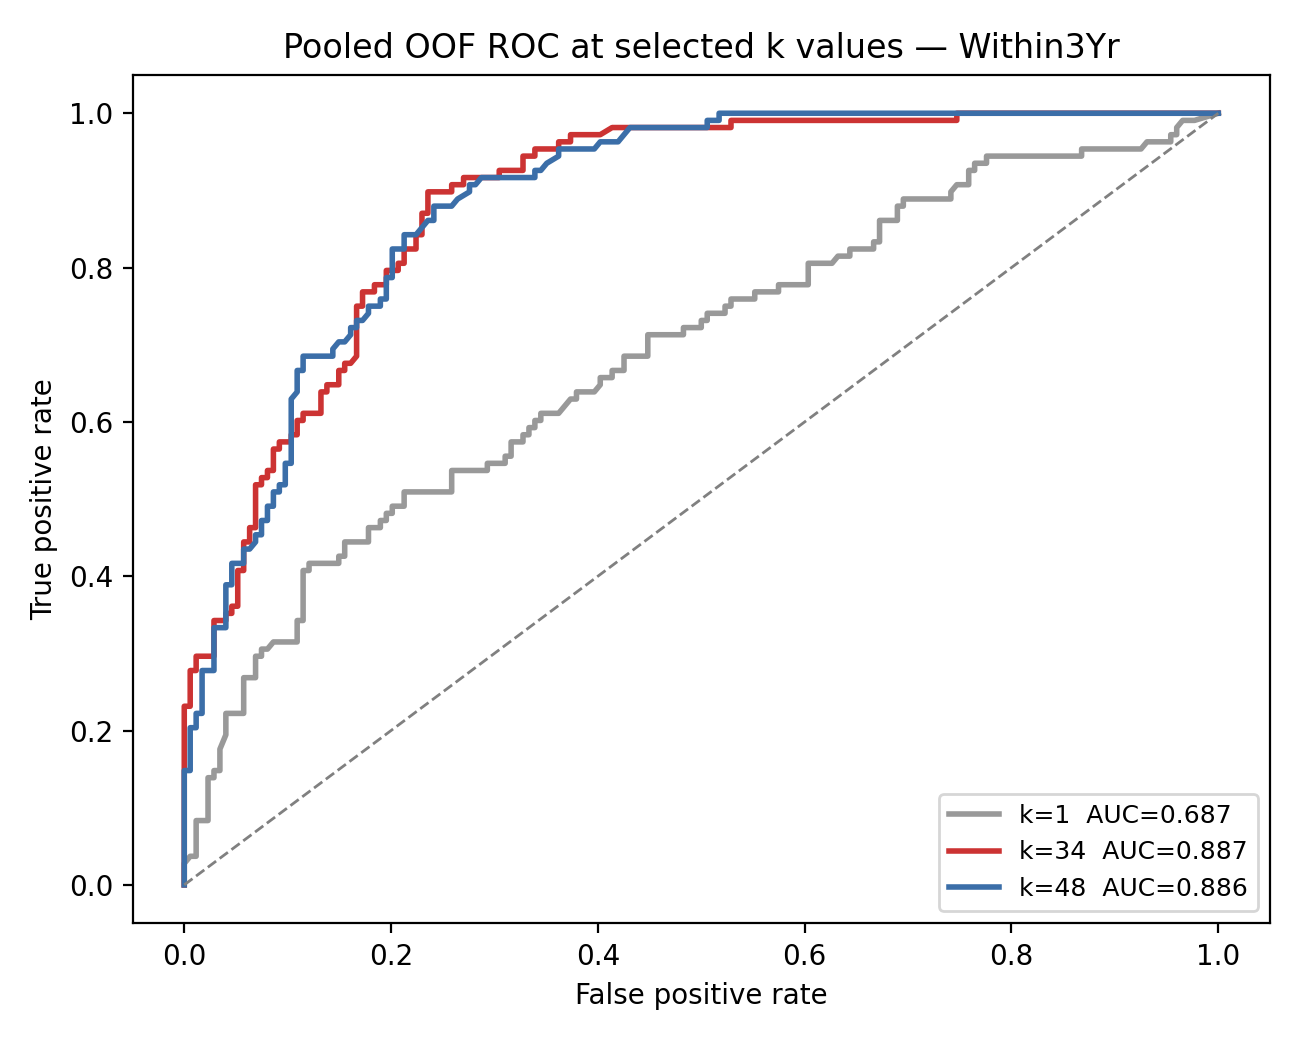
\includegraphics[width=0.62\textwidth]{gradual_roc_within3yr.png}
  \caption{Pooled OOF ROC for Within3Yr at $k=1$, peak-AUC $k$, and
  $k=|\mathcal{F}|$.}
  \label{fig:gradual_roc_within3yr}
\end{figure}

The fold-by-feature heatmap of \Cref{fig:gradual_heatmap_within3yr}
visualises where the variance lives. Some folds (e.g.\ rows $7$ and $11$)
are uniformly easy; others (e.g.\ row $14$) are uniformly hard; and the
horizontal banding shows that for any given fold, performance saturates
at intermediate $k$ rather than continuing to climb. This is exactly the
information that the across-fold-mean line aggregates over.

\begin{figure}[h]
  \centering
  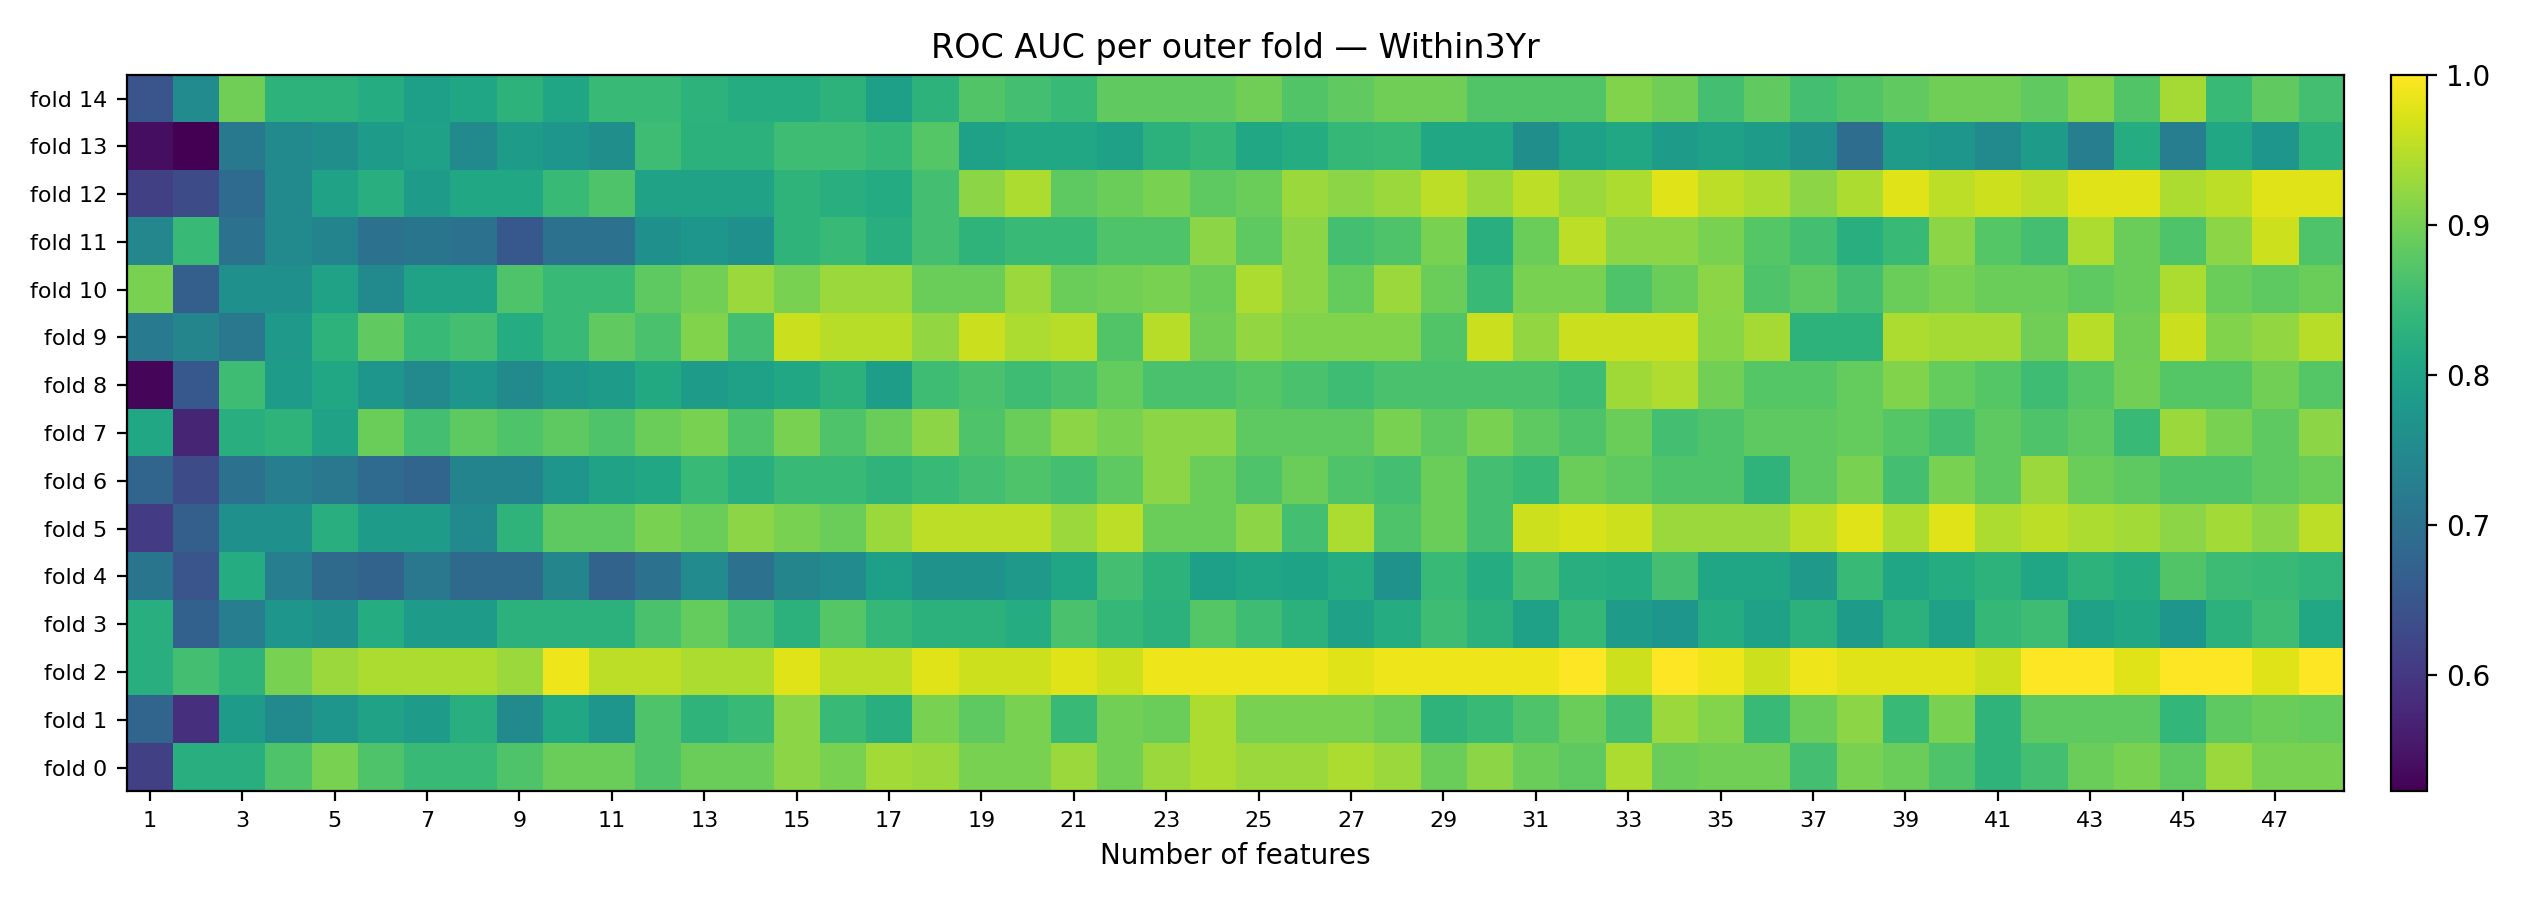
\includegraphics[width=\textwidth]{gradual_heatmap_within3yr.png}
  \caption{Per-outer-fold ROC-AUC at every feature count $k$ for
  Within3Yr. Rows are the $15$ outer folds; columns are $k$; colour is
  AUC. Most variance is across folds, not across $k$ within a fold.}
  \label{fig:gradual_heatmap_within3yr}
\end{figure}

The same pattern repeats for the most balanced horizon, Within7Yr,
which we discuss in detail in \Cref{sec:within7yr}: peak per-fold mean
AUC of $0.898$ is reached at $k=26$, and balanced accuracy peaks at
$k=19$. Across all seven horizons (\Cref{tab:gradual_summary}), the
optimal feature count for AUC ranges from $13$ to $46$, with the
median around $34$.

\begin{table}[h]
\centering
\caption{Gradual-training peak summary. Best $k$ is the feature count
that maximises the per-fold mean of the metric (minimises Brier score).
Compare $|\mathcal{F}|$ to ``Best $k$ (AUC)'' for the parsimony gap.}
\label{tab:gradual_summary}
\small
\begin{tabular}{lrrrrrrrr}
\toprule
Horizon & $|\mathcal{F}|$
        & \multicolumn{2}{c}{ROC-AUC}
        & \multicolumn{2}{c}{Balanced Acc.}
        & \multicolumn{2}{c}{$F_1$} \\
\cmidrule(lr){3-4}\cmidrule(lr){5-6}\cmidrule(lr){7-8}
        & & Best $k$ & Value & Best $k$ & Value & Best $k$ & Value \\
\midrule
Within1Yr & 33 & 13 & 0.867 &  6 & 0.723 & 14 & 0.511 \\
Within2Yr & 50 & 42 & 0.878 &  3 & 0.748 &  3 & 0.650 \\
Within3Yr & 48 & 34 & 0.898 & 23 & 0.752 & 24 & 0.683 \\
Within4Yr & 38 & 16 & 0.892 & 17 & 0.813 & 17 & 0.785 \\
Within5Yr & 46 & 46 & 0.878 &  8 & 0.804 &  8 & 0.807 \\
Within6Yr & 50 & 41 & 0.876 & 13 & 0.796 & 13 & 0.824 \\
Within7Yr & 49 & 26 & 0.898 & 19 & 0.810 & 46 & 0.863 \\
\bottomrule
\end{tabular}
\end{table}

\subsection{Cross-horizon synthesis}
\Cref{fig:summary} aggregates the per-horizon peaks. The left panel shows
the optimal feature count per metric, the right panel the corresponding
peak metric value. Two qualitative observations stand out:
\begin{enumerate}[leftmargin=*]
  \item \emph{Best $k$ is usually well below $|\mathcal{F}|$.} For
    Balanced Accuracy and $F_1$, the optimum is reached with as few as
    $3$--$25$ features in every horizon --- considerably below the
    $30$--$50$ feature size of the published lists.
  \item \emph{Peak performance does not deteriorate monotonically with
    horizon.} The longest, most balanced horizons (Within6Yr and
    Within7Yr) have the highest pooled-AP values ($\approx 0.92$--$0.94$),
    consistent with the easier-to-discriminate, more balanced label
    distributions.
\end{enumerate}

\begin{figure}[h]
  \centering
  \begin{subfigure}[t]{0.48\textwidth}
    \centering
    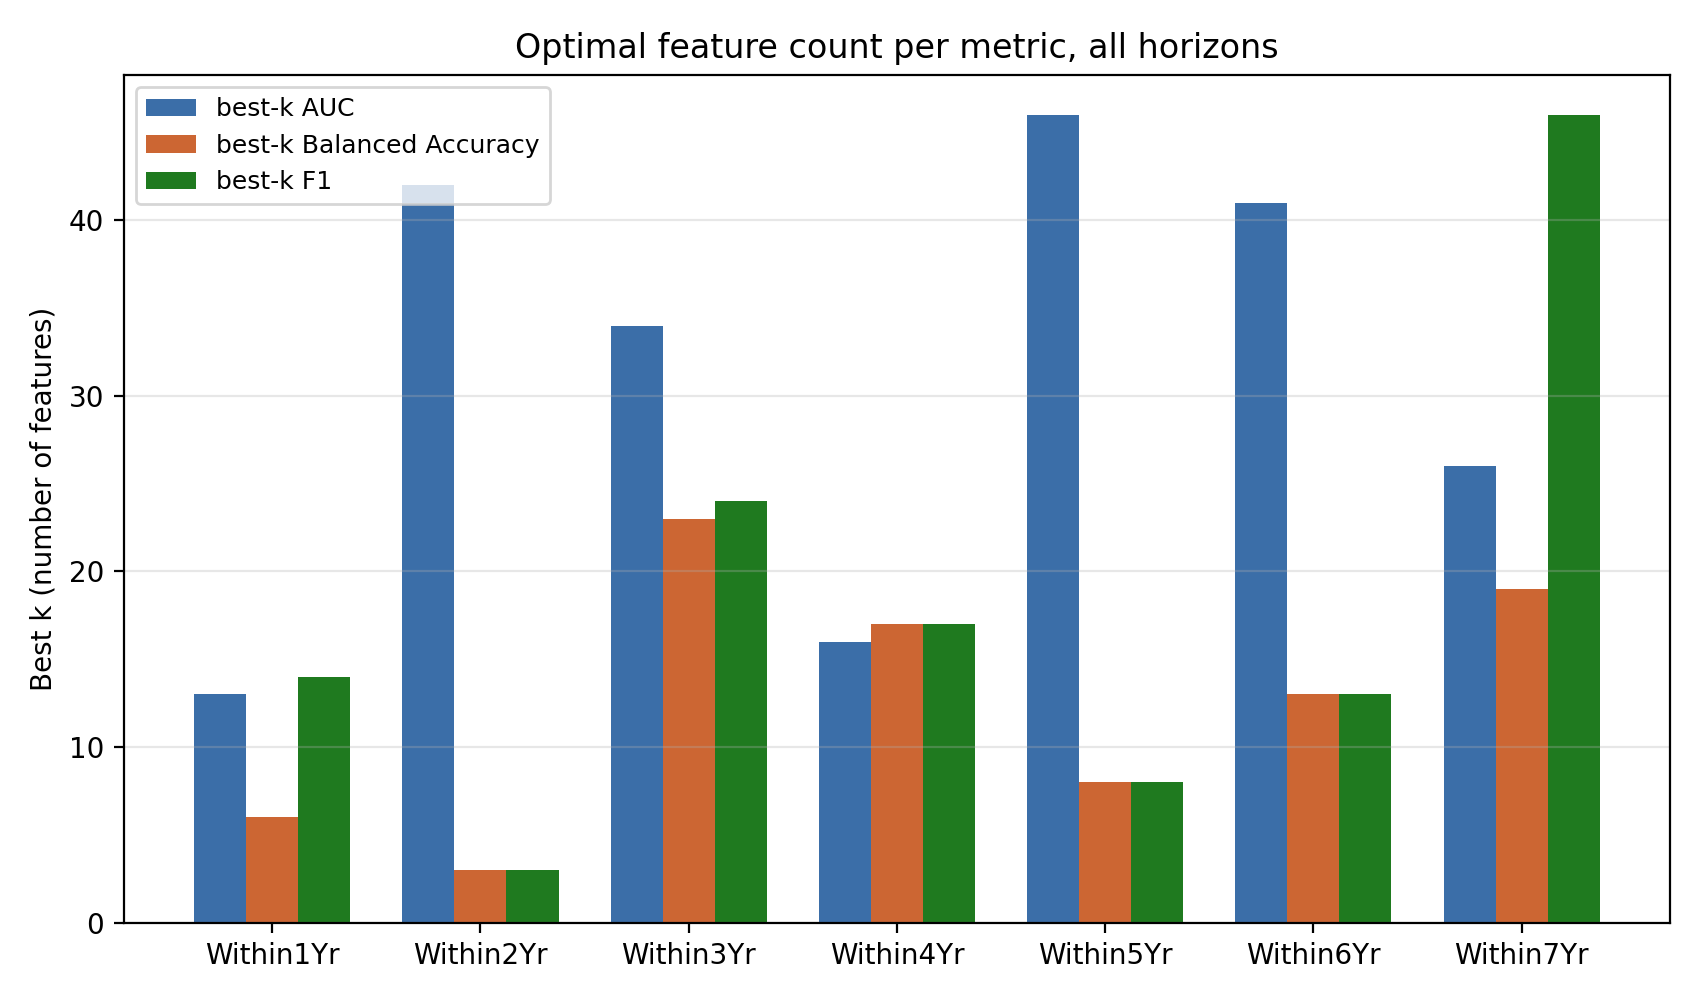
\includegraphics[width=\linewidth]{summary_best_k.png}
    \caption{Best $k$ per horizon, per metric.}
  \end{subfigure}
  \hfill
  \begin{subfigure}[t]{0.48\textwidth}
    \centering
    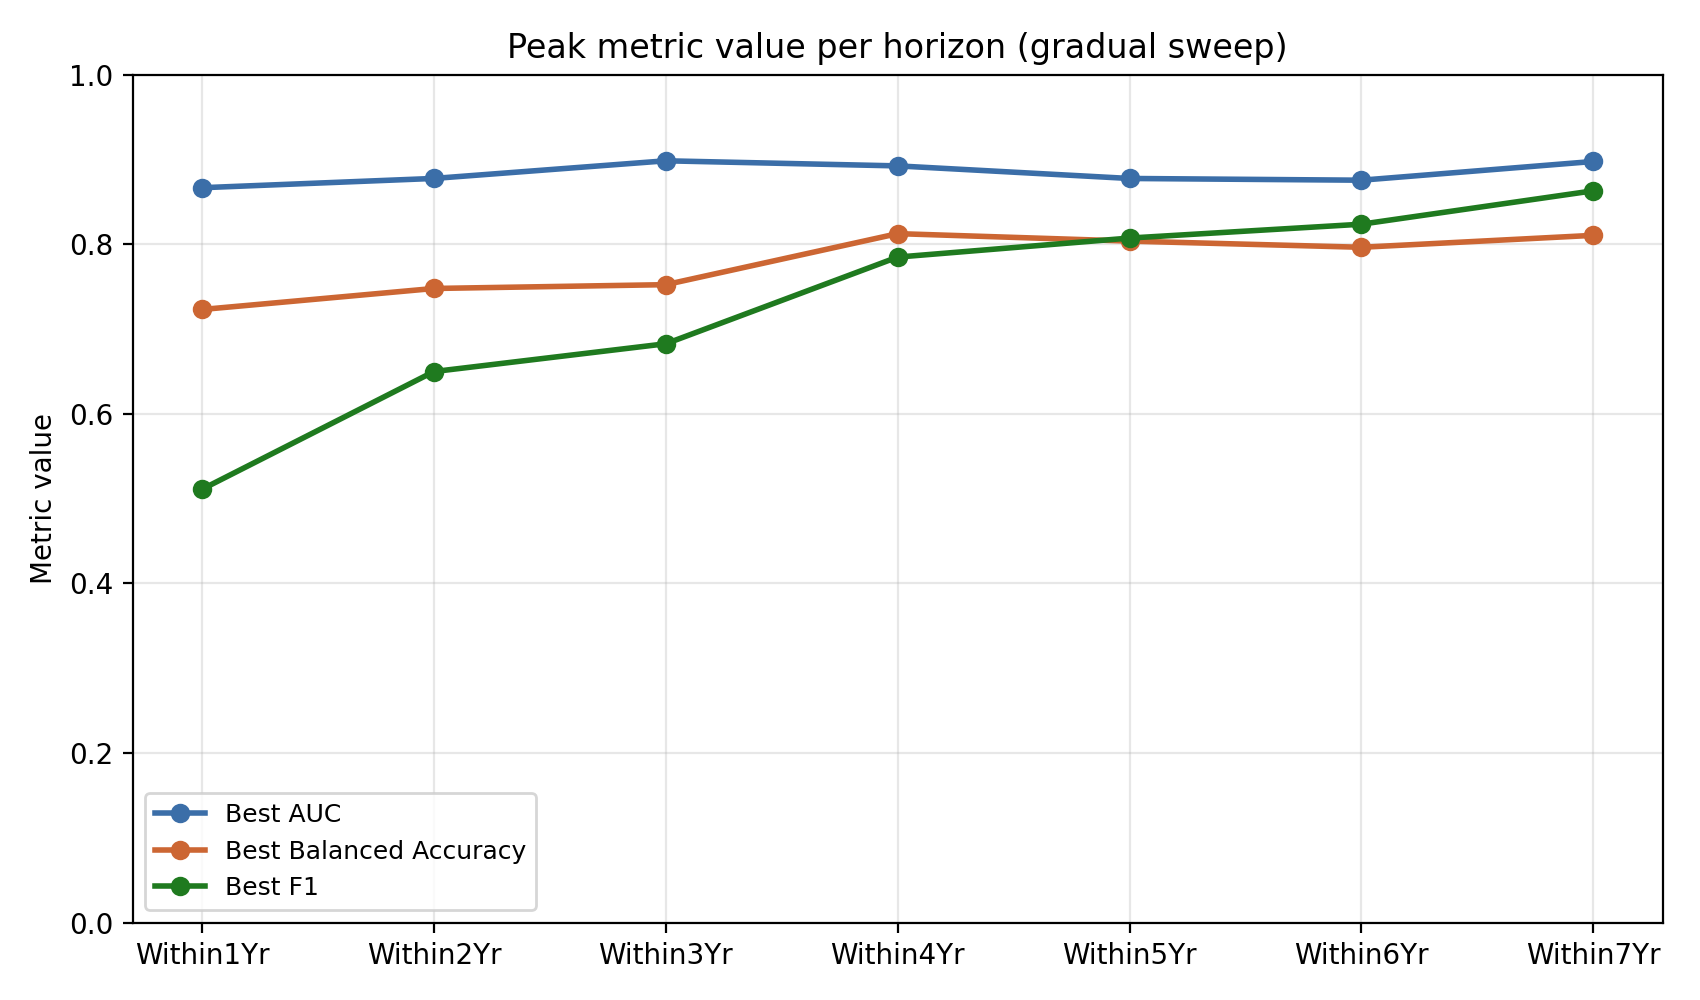
\includegraphics[width=\linewidth]{summary_best_metric_value.png}
    \caption{Peak metric value per horizon.}
  \end{subfigure}
  \caption{Cross-horizon synthesis of the gradual sweep. Left: optimal
  feature count per metric by horizon. Right: the metric value at that
  optimum.}
  \label{fig:summary}
\end{figure}

\subsection{The published feature signature}
The top-30 RF-importance features fed into the gradual sweep for
Within3Yr are shown in \Cref{fig:features_within3yr}. The ranking
includes a mix of well-known cardiovascular biomarkers (\texttt{GDF-15},
\texttt{MMP-3}, \texttt{FABP2}, \texttt{NT-proBNP}-related families) and
less-explored proteomic candidates (\texttt{LAG3}, \texttt{CD83},
\texttt{179\_EGFR}). Detailed biological discussion is deferred to a
companion clinical write-up.

\begin{figure}[h]
  \centering
  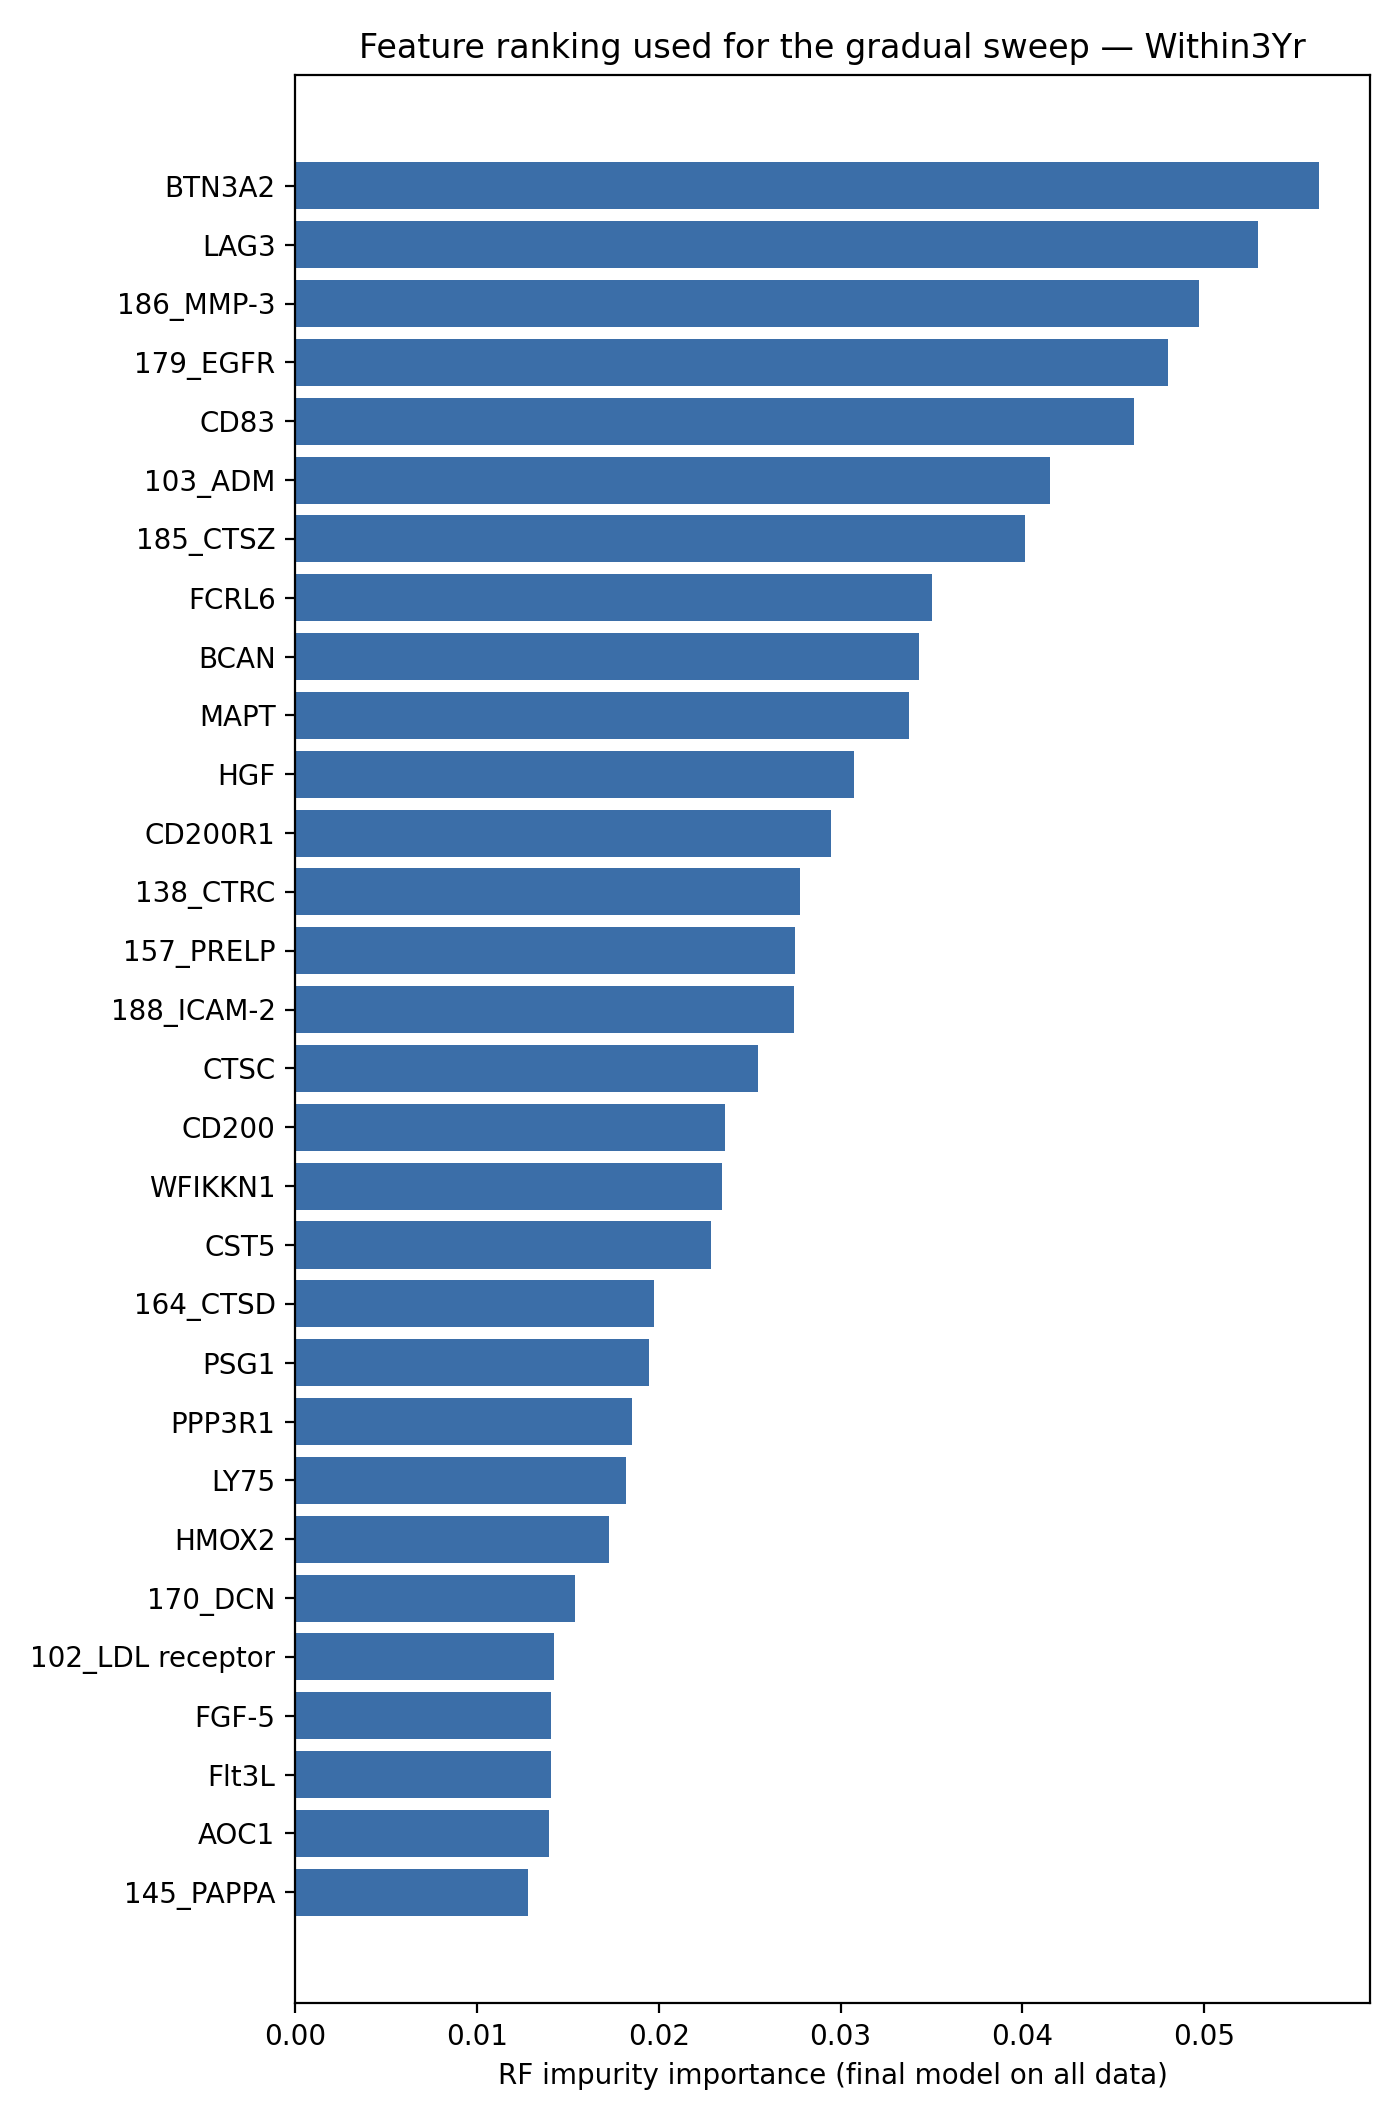
\includegraphics[width=0.85\textwidth]{gradual_features_within3yr.png}
  \caption{Top-30 features by Random-Forest impurity importance,
  Within3Yr horizon --- the ordering used for the gradual sweep.}
  \label{fig:features_within3yr}
\end{figure}

% =============================================================================
\section{Discussion}
\label{sec:discussion}

\paragraph{What the gradual sweep tells us.}
The dominant message of \Cref{tab:gradual_summary} is parsimony: across
all seven horizons, peak held-out performance is reached well before the
full stability-selected list is consumed. For Within4Yr, peak AUC is
achieved at $k=16$ from a list of size $38$; for Within3Yr at $k=34$
from $48$; for Within6Yr at $k=41$ from $50$. The held-out curves are
either monotonically increasing then flat, or single-peaked, which is the
expected shape under a regime in which the early features carry most
of the marginal information and the later features mostly add variance.

\paragraph{Caveats on optimism.}
Choosing the $k$ that maximises a sample-mean curve is itself a model
selection step, and the resulting peak value is mildly upward-biased ---
particularly for the metrics with bumpier curves
(\Cref{fig:gradual_within3yr}). The reported peak values should
therefore be interpreted as ``best achievable along this published
ranking'', not as expected out-of-sample performance for a deployment
trained at $k^\star$.

\paragraph{Why the gradual peaks exceed the main-pipeline numbers, and
why the gap is family-specific.}
A reader comparing \Cref{tab:headline} ($k=|\mathcal{F}|$ pooled AUC) to
\Cref{tab:gradual_summary} (Random-Forest gradual peak) will see the
gradual peaks several points of AUC higher; the same reader comparing
\Cref{tab:cross_model_main} to \Cref{tab:cross_model_gradual} will see
that for the linear and kernel families the gap is enormous (peaks near
$1.0$). The combined explanation has three components: (i) the gradual
ranking is computed once on the full data (\Cref{sec:gradual}), which
contributes a small look-ahead --- but, importantly, the \emph{model} at
every $k$ is still trained and evaluated under fold-respecting nested
CV; (ii) the main pipeline re-runs stability selection inside every
outer fold, so the feature set fluctuates with the fold, while the
gradual sweep holds it fixed --- holding the feature set constant
across folds removes a real source of variance and lifts the peak by a
modest amount; (iii) the magnitude of the lift depends on \emph{how
tightly the importance score used for the ranking is coupled to the
model's optimisation criterion}. Tree importance scores (RF impurity,
XGBoost gain) are coarse summaries of how often a feature is split on
and only mildly predict held-out accuracy; linear and kernel importance
scores (the LR's $|$standardised coefficient$|$ and the RBF SVM's
permutation importance) are sufficient statistics of the global model's
decision function, so reselecting the top-$k$ features by such a score
and refitting the same family is much closer to ``recover the global
model'' than to ``walk down a generic ranking''. The result is the very
clean stratification we observed in
\Cref{fig:cross_model_gap}: $+0.15$--$0.25$ for trees,
$+0.30$--$0.40$ for linear/kernel.

This is, to our knowledge, a previously unappreciated risk in
multi-model proteomic / radiomic studies that report a
``post-selection re-evaluation'' or a ``feature-count sensitivity''
analysis: the same procedure that produces a small,
correctly-interpreted bias for trees can produce a numerically
convincing but content-free curve for linear or kernel models. The fix
is conceptually simple --- recompute the ranking inside every outer
fold, which moves the analysis from sensitivity-on-rank to nested
selection --- but it changes the question being asked, which is why we
have left both interpretations open and reported the unbiased main
pipeline as the headline.

\paragraph{Class imbalance.}
Class-weight balancing is essential for Within1Yr ($\sim18\%$
positives), where an unweighted Random Forest defaults to predicting
the majority class on small training folds. This is consistent with the
near-zero recall at $\tau=0.5$ for Within1Yr in \Cref{tab:headline}; the
Youden-optimal threshold (reported in the JSON outputs) recovers a
clinically usable operating point.

% =============================================================================
\section{Limitations and future work}
\label{sec:limitations}

\begin{itemize}[leftmargin=*]
  \item \emph{Sample size.} $n=94$ is small for a $551$-feature panel.
    The width of the $\pm 1$ SD bands in \Cref{fig:gradual_within3yr}
    is the most honest summary of how much we should trust adjacent
    points on the $k$-vs-AUC curve.
  \item \emph{Single-cohort.} No external validation cohort is available.
    Reproducing the gradual peaks on a held-out independent dataset is
    the most important next step.
  \item \emph{Binary horizons.} The seven outcomes are encoded as
    binary indicators rather than time-to-event; a Cox-style or
    discrete-time-survival reformulation would account for censoring.
  \item \emph{Calibration.} Brier score is reported but no
    Platt/isotonic recalibration is applied. For a deployment-oriented
    follow-up, calibration is essential.
  \item \emph{Calibration disparity across families.} The four families
    are similar in AUC but differ noticeably in pooled Brier
    (\Cref{fig:cross_model_brier}), with linear / kernel models worse
    calibrated than tree models. A platt or isotonic recalibration
    layer should be added before any deployment.
  \item \emph{Rank-on-full-data look-ahead.} The gradual sweep uses the
    family's own published ranking computed on the full data; for
    linear and kernel families this introduces a substantial
    rank-induced bias (\Cref{sec:cross_model_gradual},
    \Cref{tab:cross_model_gradual}). A nested-selection variant of the
    sweep --- recomputing the ranking inside every outer fold --- would
    fix this at the cost of reinterpreting the analysis as nested
    feature selection rather than as a description of the published
    list.
\end{itemize}

% =============================================================================
\section{Conclusion}
\label{sec:conclusion}

We presented a leakage-free, nested-cross-validated, stability-selected
\emph{multi-model} pipeline for predicting MACE within 1--7 years from a
baseline proteomic panel of $551$ candidate features in $94$ patients.
Four classifier families --- Random Forest, XGBoost, Logistic Regression,
and an RBF-kernel SVM --- are trained, tuned, and evaluated under the
\emph{same} outer/inner cross-validation, the \emph{same}
stability-selection front-end, the \emph{same} metric battery, and the
\emph{same} fixed seed; differences in the headline numbers are therefore
attributable to the model and not to confounded preprocessing choices. A
gradual-training extension resolves, per family, how held-out
performance varies with the size of the feature signature.

Three findings stand out. \emph{First,} headline pooled AUC is broadly
comparable across the four families (range $\sim 0.06$ at any horizon)
and is dominated by data-limited rather than model-limited variance:
the per-fold standard deviation alone is $0.07$--$0.10$. \emph{Second,}
the dominant qualitative pattern in the gradual sweeps is parsimony ---
peak held-out performance is reached well before the full
stability-selected list is consumed for every (family, horizon) pair,
suggesting a much shorter, more interpretable signature would carry
most of the clinical information once external validation is available.
\emph{Third,} the size of the gradual peaks is family-specific and
reveals a previously underappreciated rank-induced look-ahead: the
gradual peaks for the linear and kernel families approach $1.0$ AUC
because their importance scores are sufficient statistics of the global
model's decision function, while the tree-based families show a much
milder, scientifically interpretable lift. We therefore anchor headline
numbers on the unbiased main pipeline and treat the gradual sweep as a
sensitivity-on-rank analysis, which is most informative for the
tree-based families.

\paragraph{Reproducibility.}
All source code, configuration, fitted artefacts, fold-level metrics,
per-patient out-of-fold predictions, and plot suites are available in
the project repository. A single fixed random seed
($\texttt{RANDOM\_STATE}=42$) is propagated through every stochastic
component of the pipeline.

% =============================================================================
% Citations and related work — placeholder for now (to be expanded later).
% =============================================================================
% \bibliographystyle{plainnat}
% \bibliography{references}

\end{document}
